\documentclass[twoside]{book}

% Packages required by doxygen
\usepackage{fixltx2e}
\usepackage{calc}
\usepackage{doxygen}
\usepackage[export]{adjustbox} % also loads graphicx
\usepackage{graphicx}
\usepackage[utf8]{inputenc}
\usepackage{makeidx}
\usepackage{multicol}
\usepackage{multirow}
\PassOptionsToPackage{warn}{textcomp}
\usepackage{textcomp}
\usepackage[nointegrals]{wasysym}
\usepackage[table]{xcolor}

% Font selection
\usepackage[T1]{fontenc}
\usepackage[scaled=.90]{helvet}
\usepackage{courier}
\usepackage{amssymb}
\usepackage{sectsty}
\renewcommand{\familydefault}{\sfdefault}
\allsectionsfont{%
  \fontseries{bc}\selectfont%
  \color{darkgray}%
}
\renewcommand{\DoxyLabelFont}{%
  \fontseries{bc}\selectfont%
  \color{darkgray}%
}
\newcommand{\+}{\discretionary{\mbox{\scriptsize$\hookleftarrow$}}{}{}}

% Page & text layout
\usepackage{geometry}
\geometry{%
  a4paper,%
  top=2.5cm,%
  bottom=2.5cm,%
  left=2.5cm,%
  right=2.5cm%
}
\tolerance=750
\hfuzz=15pt
\hbadness=750
\setlength{\emergencystretch}{15pt}
\setlength{\parindent}{0cm}
\setlength{\parskip}{3ex plus 2ex minus 2ex}
\makeatletter
\renewcommand{\paragraph}{%
  \@startsection{paragraph}{4}{0ex}{-1.0ex}{1.0ex}{%
    \normalfont\normalsize\bfseries\SS@parafont%
  }%
}
\renewcommand{\subparagraph}{%
  \@startsection{subparagraph}{5}{0ex}{-1.0ex}{1.0ex}{%
    \normalfont\normalsize\bfseries\SS@subparafont%
  }%
}
\makeatother

% Headers & footers
\usepackage{fancyhdr}
\pagestyle{fancyplain}
\fancyhead[LE]{\fancyplain{}{\bfseries\thepage}}
\fancyhead[CE]{\fancyplain{}{}}
\fancyhead[RE]{\fancyplain{}{\bfseries\leftmark}}
\fancyhead[LO]{\fancyplain{}{\bfseries\rightmark}}
\fancyhead[CO]{\fancyplain{}{}}
\fancyhead[RO]{\fancyplain{}{\bfseries\thepage}}
\fancyfoot[LE]{\fancyplain{}{}}
\fancyfoot[CE]{\fancyplain{}{}}
\fancyfoot[RE]{\fancyplain{}{\bfseries\scriptsize Generated by Doxygen }}
\fancyfoot[LO]{\fancyplain{}{\bfseries\scriptsize Generated by Doxygen }}
\fancyfoot[CO]{\fancyplain{}{}}
\fancyfoot[RO]{\fancyplain{}{}}
\renewcommand{\footrulewidth}{0.4pt}
\renewcommand{\chaptermark}[1]{%
  \markboth{#1}{}%
}
\renewcommand{\sectionmark}[1]{%
  \markright{\thesection\ #1}%
}

% Indices & bibliography
\usepackage{natbib}
\usepackage[titles]{tocloft}
\setcounter{tocdepth}{3}
\setcounter{secnumdepth}{5}
\makeindex

% Hyperlinks (required, but should be loaded last)
\usepackage{ifpdf}
\ifpdf
  \usepackage[pdftex,pagebackref=true]{hyperref}
\else
  \usepackage[ps2pdf,pagebackref=true]{hyperref}
\fi
\hypersetup{%
  colorlinks=true,%
  linkcolor=blue,%
  citecolor=blue,%
  unicode%
}

% Custom commands
\newcommand{\clearemptydoublepage}{%
  \newpage{\pagestyle{empty}\cleardoublepage}%
}

\usepackage{caption}
\captionsetup{labelsep=space,justification=centering,font={bf},singlelinecheck=off,skip=4pt,position=top}

%===== C O N T E N T S =====

\begin{document}

% Titlepage & ToC
\hypersetup{pageanchor=false,
             bookmarksnumbered=true,
             pdfencoding=unicode
            }
\pagenumbering{alph}
\begin{titlepage}
\vspace*{7cm}
\begin{center}%
{\Large District\+Heating\+System }\\
\vspace*{1cm}
{\large Generated by Doxygen 1.8.13}\\
\end{center}
\end{titlepage}
\clearemptydoublepage
\pagenumbering{roman}
\tableofcontents
\clearemptydoublepage
\pagenumbering{arabic}
\hypersetup{pageanchor=true}

%--- Begin generated contents ---
\chapter{Namespace Index}
\section{Namespace List}
Here is a list of all namespaces with brief descriptions\+:\begin{DoxyCompactList}
\item\contentsline{section}{\hyperlink{namespace_consumer}{Consumer} }{\pageref{namespace_consumer}}{}
\item\contentsline{section}{\hyperlink{namespace_data_i_o}{Data\+IO} }{\pageref{namespace_data_i_o}}{}
\item\contentsline{section}{\hyperlink{namespacedbf_input_stanet}{dbf\+Input\+Stanet} }{\pageref{namespacedbf_input_stanet}}{}
\item\contentsline{section}{\hyperlink{namespace_dictionary}{Dictionary} }{\pageref{namespace_dictionary}}{}
\item\contentsline{section}{\hyperlink{namespace_district_heating_system}{District\+Heating\+System} }{\pageref{namespace_district_heating_system}}{}
\item\contentsline{section}{\hyperlink{namespacefunction}{function} }{\pageref{namespacefunction}}{}
\item\contentsline{section}{\hyperlink{namespace_heat_exchanger}{Heat\+Exchanger} }{\pageref{namespace_heat_exchanger}}{}
\item\contentsline{section}{\hyperlink{namespace_heat_grid}{Heat\+Grid} }{\pageref{namespace_heat_grid}}{}
\item\contentsline{section}{\hyperlink{namespace_heat_sink}{Heat\+Sink} }{\pageref{namespace_heat_sink}}{}
\item\contentsline{section}{\hyperlink{namespace_heat_sink___consumptionprofiles}{Heat\+Sink\+\_\+\+Consumptionprofiles} }{\pageref{namespace_heat_sink___consumptionprofiles}}{}
\item\contentsline{section}{\hyperlink{namespace_heat_source}{Heat\+Source} }{\pageref{namespace_heat_source}}{}
\item\contentsline{section}{\hyperlink{namespaceimport_d_b_ffrom_s_t_a_n_e_t}{import\+D\+B\+Ffrom\+S\+T\+A\+N\+ET} }{\pageref{namespaceimport_d_b_ffrom_s_t_a_n_e_t}}{}
\item\contentsline{section}{\hyperlink{namespaceinzidenzmatrix}{inzidenzmatrix} }{\pageref{namespaceinzidenzmatrix}}{}
\item\contentsline{section}{\hyperlink{namespace_main}{Main} }{\pageref{namespace_main}}{}
\item\contentsline{section}{\hyperlink{namespace_node}{Node} }{\pageref{namespace_node}}{}
\item\contentsline{section}{\hyperlink{namespace_pipe}{Pipe} }{\pageref{namespace_pipe}}{}
\item\contentsline{section}{\hyperlink{namespace_producer}{Producer} }{\pageref{namespace_producer}}{}
\item\contentsline{section}{\hyperlink{namespace_pump}{Pump} }{\pageref{namespace_pump}}{}
\item\contentsline{section}{\hyperlink{namespace_s_t_a_n_e_t___d_b_fto_class}{S\+T\+A\+N\+E\+T\+\_\+\+D\+B\+Fto\+Class} }{\pageref{namespace_s_t_a_n_e_t___d_b_fto_class}}{}
\item\contentsline{section}{\hyperlink{namespacetest}{test} }{\pageref{namespacetest}}{}
\item\contentsline{section}{\hyperlink{namespacetest_pipe}{test\+Pipe} }{\pageref{namespacetest_pipe}}{}
\end{DoxyCompactList}

\chapter{Class Index}
\section{Class List}
Here are the classes, structs, unions and interfaces with brief descriptions\+:\begin{DoxyCompactList}
\item\contentsline{section}{\hyperlink{class_consumer_1_1_consumer}{Consumer.\+Consumer} }{\pageref{class_consumer_1_1_consumer}}{}
\item\contentsline{section}{\hyperlink{class_data_i_o_1_1_data_i_o}{Data\+I\+O.\+Data\+IO} }{\pageref{class_data_i_o_1_1_data_i_o}}{}
\item\contentsline{section}{\hyperlink{class_district_heating_system_1_1_district_heating_system}{District\+Heating\+System.\+District\+Heating\+System} }{\pageref{class_district_heating_system_1_1_district_heating_system}}{}
\item\contentsline{section}{\hyperlink{class_heat_exchanger_1_1_heat_exchanger}{Heat\+Exchanger.\+Heat\+Exchanger} }{\pageref{class_heat_exchanger_1_1_heat_exchanger}}{}
\item\contentsline{section}{\hyperlink{class_heat_grid_1_1_heat_grid}{Heat\+Grid.\+Heat\+Grid} }{\pageref{class_heat_grid_1_1_heat_grid}}{}
\item\contentsline{section}{\hyperlink{class_heat_sink_1_1_heat_sink}{Heat\+Sink.\+Heat\+Sink} }{\pageref{class_heat_sink_1_1_heat_sink}}{}
\item\contentsline{section}{\hyperlink{class_heat_sink___consumptionprofiles_1_1_heat_sink___consumptionprofiles}{Heat\+Sink\+\_\+\+Consumptionprofiles.\+Heat\+Sink\+\_\+\+Consumptionprofiles} }{\pageref{class_heat_sink___consumptionprofiles_1_1_heat_sink___consumptionprofiles}}{}
\item\contentsline{section}{\hyperlink{class_heat_source_1_1_heat_source}{Heat\+Source.\+Heat\+Source} }{\pageref{class_heat_source_1_1_heat_source}}{}
\item\contentsline{section}{\hyperlink{class_node_1_1_node}{Node.\+Node} }{\pageref{class_node_1_1_node}}{}
\item\contentsline{section}{\hyperlink{class_pipe_1_1_pipe}{Pipe.\+Pipe} }{\pageref{class_pipe_1_1_pipe}}{}
\item\contentsline{section}{\hyperlink{class_producer_1_1_producer}{Producer.\+Producer} }{\pageref{class_producer_1_1_producer}}{}
\item\contentsline{section}{\hyperlink{class_pump_1_1_pump}{Pump.\+Pump} }{\pageref{class_pump_1_1_pump}}{}
\item\contentsline{section}{\hyperlink{classtest_1_1test}{test.\+test} }{\pageref{classtest_1_1test}}{}
\end{DoxyCompactList}

\chapter{File Index}
\section{File List}
Here is a list of all files with brief descriptions\+:\begin{DoxyCompactList}
\item\contentsline{section}{C\+:/\+Users/jpelda/\+Documents/\+Git\+Hub/district\+Heating/\hyperlink{_main_8py}{Main.\+py} }{\pageref{_main_8py}}{}
\item\contentsline{section}{C\+:/\+Users/jpelda/\+Documents/\+Git\+Hub/district\+Heating/class/\hyperlink{_consumer_8py}{Consumer.\+py} }{\pageref{_consumer_8py}}{}
\item\contentsline{section}{C\+:/\+Users/jpelda/\+Documents/\+Git\+Hub/district\+Heating/class/\hyperlink{_data_i_o_8py}{Data\+I\+O.\+py} }{\pageref{_data_i_o_8py}}{}
\item\contentsline{section}{C\+:/\+Users/jpelda/\+Documents/\+Git\+Hub/district\+Heating/class/\hyperlink{_dictionary_8py}{Dictionary.\+py} }{\pageref{_dictionary_8py}}{}
\item\contentsline{section}{C\+:/\+Users/jpelda/\+Documents/\+Git\+Hub/district\+Heating/class/\hyperlink{_district_heating_system_8py}{District\+Heating\+System.\+py} }{\pageref{_district_heating_system_8py}}{}
\item\contentsline{section}{C\+:/\+Users/jpelda/\+Documents/\+Git\+Hub/district\+Heating/class/\hyperlink{function_8py}{function.\+py} }{\pageref{function_8py}}{}
\item\contentsline{section}{C\+:/\+Users/jpelda/\+Documents/\+Git\+Hub/district\+Heating/class/\hyperlink{_heat_exchanger_8py}{Heat\+Exchanger.\+py} }{\pageref{_heat_exchanger_8py}}{}
\item\contentsline{section}{C\+:/\+Users/jpelda/\+Documents/\+Git\+Hub/district\+Heating/class/\hyperlink{_heat_grid_8py}{Heat\+Grid.\+py} }{\pageref{_heat_grid_8py}}{}
\item\contentsline{section}{C\+:/\+Users/jpelda/\+Documents/\+Git\+Hub/district\+Heating/class/\hyperlink{_heat_sink_8py}{Heat\+Sink.\+py} }{\pageref{_heat_sink_8py}}{}
\item\contentsline{section}{C\+:/\+Users/jpelda/\+Documents/\+Git\+Hub/district\+Heating/class/\hyperlink{_heat_sink___consumptionprofiles_8py}{Heat\+Sink\+\_\+\+Consumptionprofiles.\+py} }{\pageref{_heat_sink___consumptionprofiles_8py}}{}
\item\contentsline{section}{C\+:/\+Users/jpelda/\+Documents/\+Git\+Hub/district\+Heating/class/\hyperlink{_heat_source_8py}{Heat\+Source.\+py} }{\pageref{_heat_source_8py}}{}
\item\contentsline{section}{C\+:/\+Users/jpelda/\+Documents/\+Git\+Hub/district\+Heating/class/\hyperlink{_node_8py}{Node.\+py} }{\pageref{_node_8py}}{}
\item\contentsline{section}{C\+:/\+Users/jpelda/\+Documents/\+Git\+Hub/district\+Heating/class/\hyperlink{_pipe_8py}{Pipe.\+py} }{\pageref{_pipe_8py}}{}
\item\contentsline{section}{C\+:/\+Users/jpelda/\+Documents/\+Git\+Hub/district\+Heating/class/\hyperlink{_producer_8py}{Producer.\+py} }{\pageref{_producer_8py}}{}
\item\contentsline{section}{C\+:/\+Users/jpelda/\+Documents/\+Git\+Hub/district\+Heating/class/\hyperlink{_pump_8py}{Pump.\+py} }{\pageref{_pump_8py}}{}
\item\contentsline{section}{C\+:/\+Users/jpelda/\+Documents/\+Git\+Hub/district\+Heating/class/\hyperlink{test_8py}{test.\+py} }{\pageref{test_8py}}{}
\item\contentsline{section}{C\+:/\+Users/jpelda/\+Documents/\+Git\+Hub/district\+Heating/class/\+Data\+I\+O/\hyperlink{import_d_b_ffrom_s_t_a_n_e_t_8py}{import\+D\+B\+Ffrom\+S\+T\+A\+N\+E\+T.\+py} }{\pageref{import_d_b_ffrom_s_t_a_n_e_t_8py}}{}
\item\contentsline{section}{C\+:/\+Users/jpelda/\+Documents/\+Git\+Hub/district\+Heating/function/\hyperlink{dbf_input_stanet_8py}{dbf\+Input\+Stanet.\+py} }{\pageref{dbf_input_stanet_8py}}{}
\item\contentsline{section}{C\+:/\+Users/jpelda/\+Documents/\+Git\+Hub/district\+Heating/function/\hyperlink{inzidenzmatrix_8py}{inzidenzmatrix.\+py} }{\pageref{inzidenzmatrix_8py}}{}
\item\contentsline{section}{C\+:/\+Users/jpelda/\+Documents/\+Git\+Hub/district\+Heating/function/\hyperlink{_s_t_a_n_e_t___d_b_fto_class_8py}{S\+T\+A\+N\+E\+T\+\_\+\+D\+B\+Fto\+Class.\+py} }{\pageref{_s_t_a_n_e_t___d_b_fto_class_8py}}{}
\item\contentsline{section}{C\+:/\+Users/jpelda/\+Documents/\+Git\+Hub/district\+Heating/test/\hyperlink{test_pipe_8py}{test\+Pipe.\+py} }{\pageref{test_pipe_8py}}{}
\end{DoxyCompactList}

\chapter{Namespace Documentation}
\hypertarget{namespace_consumer}{}\section{Consumer Namespace Reference}
\label{namespace_consumer}\index{Consumer@{Consumer}}
\subsection*{Classes}
\begin{DoxyCompactItemize}
\item 
class \hyperlink{class_consumer_1_1_consumer}{Consumer}
\end{DoxyCompactItemize}

\hypertarget{namespace_data_i_o}{}\section{Data\+IO Namespace Reference}
\label{namespace_data_i_o}\index{Data\+IO@{Data\+IO}}
\subsection*{Classes}
\begin{DoxyCompactItemize}
\item 
class \hyperlink{class_data_i_o_1_1_data_i_o}{Data\+IO}
\end{DoxyCompactItemize}

\hypertarget{namespacedbf_input_stanet}{}\section{dbf\+Input\+Stanet Namespace Reference}
\label{namespacedbf_input_stanet}\index{dbf\+Input\+Stanet@{dbf\+Input\+Stanet}}
\subsection*{Functions}
\begin{DoxyCompactItemize}
\item 
def \hyperlink{namespacedbf_input_stanet_a33ccd8626c4dfbd223fa22ae27efdd8d}{get\+Pipe} (name\+Pipe)
\item 
def \hyperlink{namespacedbf_input_stanet_a1df8b485c2384b611f5ec1c3eb97653b}{get\+Node} (name\+Node)
\item 
def \hyperlink{namespacedbf_input_stanet_ab3508db83b066e71bc0a35e7fb3684ef}{get\+Heat\+Exchanger} (name\+Heat\+Exchanger)
\end{DoxyCompactItemize}
\subsection*{Variables}
\begin{DoxyCompactItemize}
\item 
\hyperlink{namespacedbf_input_stanet_af54a8f3f60e0d2930e153f8cdcc7d5d6}{url} = os.\+path.\+join(os.\+path.\+abspath(\char`\"{}.\char`\"{}) , os.\+path.\+join(\textquotesingle{}input\textquotesingle{}, \textquotesingle{}Test\+Netz\textquotesingle{}))
\end{DoxyCompactItemize}


\subsection{Function Documentation}
\mbox{\Hypertarget{namespacedbf_input_stanet_ab3508db83b066e71bc0a35e7fb3684ef}\label{namespacedbf_input_stanet_ab3508db83b066e71bc0a35e7fb3684ef}} 
\index{dbf\+Input\+Stanet@{dbf\+Input\+Stanet}!get\+Heat\+Exchanger@{get\+Heat\+Exchanger}}
\index{get\+Heat\+Exchanger@{get\+Heat\+Exchanger}!dbf\+Input\+Stanet@{dbf\+Input\+Stanet}}
\subsubsection{\texorpdfstring{get\+Heat\+Exchanger()}{getHeatExchanger()}}
{\footnotesize\ttfamily def dbf\+Input\+Stanet.\+get\+Heat\+Exchanger (\begin{DoxyParamCaption}\item[{}]{name\+Heat\+Exchanger }\end{DoxyParamCaption})}



Definition at line 51 of file dbf\+Input\+Stanet.\+py.

\mbox{\Hypertarget{namespacedbf_input_stanet_a1df8b485c2384b611f5ec1c3eb97653b}\label{namespacedbf_input_stanet_a1df8b485c2384b611f5ec1c3eb97653b}} 
\index{dbf\+Input\+Stanet@{dbf\+Input\+Stanet}!get\+Node@{get\+Node}}
\index{get\+Node@{get\+Node}!dbf\+Input\+Stanet@{dbf\+Input\+Stanet}}
\subsubsection{\texorpdfstring{get\+Node()}{getNode()}}
{\footnotesize\ttfamily def dbf\+Input\+Stanet.\+get\+Node (\begin{DoxyParamCaption}\item[{}]{name\+Node }\end{DoxyParamCaption})}



Definition at line 38 of file dbf\+Input\+Stanet.\+py.

\mbox{\Hypertarget{namespacedbf_input_stanet_a33ccd8626c4dfbd223fa22ae27efdd8d}\label{namespacedbf_input_stanet_a33ccd8626c4dfbd223fa22ae27efdd8d}} 
\index{dbf\+Input\+Stanet@{dbf\+Input\+Stanet}!get\+Pipe@{get\+Pipe}}
\index{get\+Pipe@{get\+Pipe}!dbf\+Input\+Stanet@{dbf\+Input\+Stanet}}
\subsubsection{\texorpdfstring{get\+Pipe()}{getPipe()}}
{\footnotesize\ttfamily def dbf\+Input\+Stanet.\+get\+Pipe (\begin{DoxyParamCaption}\item[{}]{name\+Pipe }\end{DoxyParamCaption})}



Definition at line 17 of file dbf\+Input\+Stanet.\+py.



\subsection{Variable Documentation}
\mbox{\Hypertarget{namespacedbf_input_stanet_af54a8f3f60e0d2930e153f8cdcc7d5d6}\label{namespacedbf_input_stanet_af54a8f3f60e0d2930e153f8cdcc7d5d6}} 
\index{dbf\+Input\+Stanet@{dbf\+Input\+Stanet}!url@{url}}
\index{url@{url}!dbf\+Input\+Stanet@{dbf\+Input\+Stanet}}
\subsubsection{\texorpdfstring{url}{url}}
{\footnotesize\ttfamily dbf\+Input\+Stanet.\+url = os.\+path.\+join(os.\+path.\+abspath(\char`\"{}.\char`\"{}) , os.\+path.\+join(\textquotesingle{}input\textquotesingle{}, \textquotesingle{}Test\+Netz\textquotesingle{}))}



Definition at line 15 of file dbf\+Input\+Stanet.\+py.


\hypertarget{namespace_dictionary}{}\section{Dictionary Namespace Reference}
\label{namespace_dictionary}\index{Dictionary@{Dictionary}}
\subsection*{Variables}
\begin{DoxyCompactItemize}
\item 
dictionary \hyperlink{namespace_dictionary_a81817c3683d83c45721baf9ac7a0f324}{Heat\+Grid\+\_\+pipe\+\_\+dtype}
\item 
dictionary \hyperlink{namespace_dictionary_a302fe29521940f3c902f1d1be3652eea}{Heat\+Grid\+\_\+node\+\_\+dtype}
\item 
dictionary \hyperlink{namespace_dictionary_a87613937e78bcf53500a014dfffc9bef}{Heat\+Sink\+\_\+consumer\+\_\+dtype}
\item 
dictionary \hyperlink{namespace_dictionary_a616d65efc5bb5f169c0fb9781b4292c2}{Heat\+Grid\+\_\+pump\+\_\+dtype}
\item 
dictionary \hyperlink{namespace_dictionary_abeaeccad0ef3f237fd95ed21a43fa64e}{Heat\+Source\+\_\+producer\+\_\+dtype}
\item 
dictionary \hyperlink{namespace_dictionary_a716974bfb5b5b6f527f42b336c7d8a78}{S\+T\+A\+N\+E\+T\+\_\+nodes}
\item 
dictionary \hyperlink{namespace_dictionary_a57c00cf376cd84145639bfb65b4e155c}{S\+T\+A\+N\+E\+T\+\_\+pipes}
\item 
dictionary \hyperlink{namespace_dictionary_a4d548616b60c21d9481e34dc5f56ff6d}{S\+T\+A\+N\+E\+T\+\_\+consumer}
\item 
dictionary \hyperlink{namespace_dictionary_aeea7b54a3132a64d164394f80e275ee1}{S\+T\+A\+N\+E\+T\+\_\+producer}
\item 
dictionary \hyperlink{namespace_dictionary_a98301ff2458867192a5d80b8d59dfe94}{Heat\+Grid\+\_\+\+S\+T\+A\+N\+E\+T\+\_\+nodes\+\_\+allocation}
\item 
dictionary \hyperlink{namespace_dictionary_a7c7183d62ec27e3eabf3fa48e77d7cba}{Heat\+Grid\+\_\+\+S\+T\+A\+N\+E\+T\+\_\+pipes\+\_\+allocation}
\item 
dictionary \hyperlink{namespace_dictionary_a334d744a07f946e317946dbd8b5785bf}{Heat\+Sink\+\_\+\+S\+T\+A\+N\+E\+T\+\_\+consumer\+\_\+allocation}
\item 
dictionary \hyperlink{namespace_dictionary_a372356497cc875933e355473f718698c}{Pump\+\_\+\+S\+T\+A\+N\+E\+T\+\_\+consumer\+\_\+allocation}
\item 
dictionary \hyperlink{namespace_dictionary_a3edbaf1cfe1d45f0558ddc8cd934b6d3}{Heat\+Source\+\_\+\+S\+T\+A\+N\+E\+T\+\_\+producer\+\_\+allocation}
\end{DoxyCompactItemize}


\subsection{Variable Documentation}
\mbox{\Hypertarget{namespace_dictionary_a302fe29521940f3c902f1d1be3652eea}\label{namespace_dictionary_a302fe29521940f3c902f1d1be3652eea}} 
\index{Dictionary@{Dictionary}!Heat\+Grid\+\_\+node\+\_\+dtype@{Heat\+Grid\+\_\+node\+\_\+dtype}}
\index{Heat\+Grid\+\_\+node\+\_\+dtype@{Heat\+Grid\+\_\+node\+\_\+dtype}!Dictionary@{Dictionary}}
\subsubsection{\texorpdfstring{Heat\+Grid\+\_\+node\+\_\+dtype}{HeatGrid\_node\_dtype}}
{\footnotesize\ttfamily dictionary Dictionary.\+Heat\+Grid\+\_\+node\+\_\+dtype}

{\bfseries Initial value\+:}
\begin{DoxyCode}
1 =     \{\textcolor{stringliteral}{'names'}: (
2                                 \textcolor{stringliteral}{'index'},
3                                 \textcolor{stringliteral}{'x'},
4                                 \textcolor{stringliteral}{'y'},
5                                 \textcolor{stringliteral}{'name'},
6                                 \textcolor{stringliteral}{'height'},
7                                 \textcolor{stringliteral}{'SP\_RP'}
8                                 ),
9                        \textcolor{stringliteral}{'formats'}: (
10                                 \textcolor{stringliteral}{'i'},
11                                 \textcolor{stringliteral}{'f'},
12                                 \textcolor{stringliteral}{'f'},
13                                 \textcolor{stringliteral}{'U10'},
14                                 \textcolor{stringliteral}{'f'},
15                                 \textcolor{stringliteral}{'U2'},
16                                 )
17                                \}
\end{DoxyCode}


Definition at line 60 of file Dictionary.\+py.

\mbox{\Hypertarget{namespace_dictionary_a81817c3683d83c45721baf9ac7a0f324}\label{namespace_dictionary_a81817c3683d83c45721baf9ac7a0f324}} 
\index{Dictionary@{Dictionary}!Heat\+Grid\+\_\+pipe\+\_\+dtype@{Heat\+Grid\+\_\+pipe\+\_\+dtype}}
\index{Heat\+Grid\+\_\+pipe\+\_\+dtype@{Heat\+Grid\+\_\+pipe\+\_\+dtype}!Dictionary@{Dictionary}}
\subsubsection{\texorpdfstring{Heat\+Grid\+\_\+pipe\+\_\+dtype}{HeatGrid\_pipe\_dtype}}
{\footnotesize\ttfamily dictionary Dictionary.\+Heat\+Grid\+\_\+pipe\+\_\+dtype}



Definition at line 9 of file Dictionary.\+py.

\mbox{\Hypertarget{namespace_dictionary_a616d65efc5bb5f169c0fb9781b4292c2}\label{namespace_dictionary_a616d65efc5bb5f169c0fb9781b4292c2}} 
\index{Dictionary@{Dictionary}!Heat\+Grid\+\_\+pump\+\_\+dtype@{Heat\+Grid\+\_\+pump\+\_\+dtype}}
\index{Heat\+Grid\+\_\+pump\+\_\+dtype@{Heat\+Grid\+\_\+pump\+\_\+dtype}!Dictionary@{Dictionary}}
\subsubsection{\texorpdfstring{Heat\+Grid\+\_\+pump\+\_\+dtype}{HeatGrid\_pump\_dtype}}
{\footnotesize\ttfamily dictionary Dictionary.\+Heat\+Grid\+\_\+pump\+\_\+dtype}

{\bfseries Initial value\+:}
\begin{DoxyCode}
1 =     \{\textcolor{stringliteral}{'names'}: (
2                                 \textcolor{stringliteral}{'index'},
3                                 \textcolor{stringliteral}{'profil'},
4                                 \textcolor{stringliteral}{'start\_node\_name'},
5                                 \textcolor{stringliteral}{'end\_node\_name'},
6                                 \textcolor{stringliteral}{'start\_x'},
7                                 \textcolor{stringliteral}{'start\_y'},
8                                 \textcolor{stringliteral}{'end\_x'},
9                                 \textcolor{stringliteral}{'end\_y'},
10                                 ),
11                        \textcolor{stringliteral}{'formats'}: (
12                                 \textcolor{stringliteral}{'i'},
13                                 \textcolor{stringliteral}{'U30'},
14                                 \textcolor{stringliteral}{'U10'},
15                                 \textcolor{stringliteral}{'U10'},
16                                 \textcolor{stringliteral}{'f'},
17                                 \textcolor{stringliteral}{'f'},
18                                 \textcolor{stringliteral}{'f'},
19                                 \textcolor{stringliteral}{'f'},
20                                 )
21                                \}
\end{DoxyCode}


Definition at line 104 of file Dictionary.\+py.

\mbox{\Hypertarget{namespace_dictionary_a98301ff2458867192a5d80b8d59dfe94}\label{namespace_dictionary_a98301ff2458867192a5d80b8d59dfe94}} 
\index{Dictionary@{Dictionary}!Heat\+Grid\+\_\+\+S\+T\+A\+N\+E\+T\+\_\+nodes\+\_\+allocation@{Heat\+Grid\+\_\+\+S\+T\+A\+N\+E\+T\+\_\+nodes\+\_\+allocation}}
\index{Heat\+Grid\+\_\+\+S\+T\+A\+N\+E\+T\+\_\+nodes\+\_\+allocation@{Heat\+Grid\+\_\+\+S\+T\+A\+N\+E\+T\+\_\+nodes\+\_\+allocation}!Dictionary@{Dictionary}}
\subsubsection{\texorpdfstring{Heat\+Grid\+\_\+\+S\+T\+A\+N\+E\+T\+\_\+nodes\+\_\+allocation}{HeatGrid\_STANET\_nodes\_allocation}}
{\footnotesize\ttfamily dictionary Dictionary.\+Heat\+Grid\+\_\+\+S\+T\+A\+N\+E\+T\+\_\+nodes\+\_\+allocation}

{\bfseries Initial value\+:}
\begin{DoxyCode}
1 =  \{
2                                 \textcolor{stringliteral}{'x'}: \textcolor{stringliteral}{'XRECHTS'},
3                                 \textcolor{stringliteral}{'y'}: \textcolor{stringliteral}{'YHOCH'},
4                                 \textcolor{stringliteral}{'name'}: \textcolor{stringliteral}{'KNAM'}
5                                 \}
\end{DoxyCode}


Definition at line 194 of file Dictionary.\+py.

\mbox{\Hypertarget{namespace_dictionary_a7c7183d62ec27e3eabf3fa48e77d7cba}\label{namespace_dictionary_a7c7183d62ec27e3eabf3fa48e77d7cba}} 
\index{Dictionary@{Dictionary}!Heat\+Grid\+\_\+\+S\+T\+A\+N\+E\+T\+\_\+pipes\+\_\+allocation@{Heat\+Grid\+\_\+\+S\+T\+A\+N\+E\+T\+\_\+pipes\+\_\+allocation}}
\index{Heat\+Grid\+\_\+\+S\+T\+A\+N\+E\+T\+\_\+pipes\+\_\+allocation@{Heat\+Grid\+\_\+\+S\+T\+A\+N\+E\+T\+\_\+pipes\+\_\+allocation}!Dictionary@{Dictionary}}
\subsubsection{\texorpdfstring{Heat\+Grid\+\_\+\+S\+T\+A\+N\+E\+T\+\_\+pipes\+\_\+allocation}{HeatGrid\_STANET\_pipes\_allocation}}
{\footnotesize\ttfamily dictionary Dictionary.\+Heat\+Grid\+\_\+\+S\+T\+A\+N\+E\+T\+\_\+pipes\+\_\+allocation}

{\bfseries Initial value\+:}
\begin{DoxyCode}
1 =  \{
2                                 \textcolor{stringliteral}{'index'}: 0,
3                                 \textcolor{stringliteral}{'start\_x'}: 0,
4                                 \textcolor{stringliteral}{'start\_y'}: 0,
5                                 \textcolor{stringliteral}{'end\_x'}: 0,
6                                 \textcolor{stringliteral}{'end\_y'}: 0,
7                                 \textcolor{stringliteral}{'start\_node\_name'}: \textcolor{stringliteral}{'ANFNAM'},
8                                 \textcolor{stringliteral}{'end\_node\_name'}: \textcolor{stringliteral}{'ENDNAM'},
9                                 \textcolor{stringliteral}{'length'}: \textcolor{stringliteral}{'RORL'},
10                                 \textcolor{stringliteral}{'diameter\_inner'}: \textcolor{stringliteral}{'DM'},
11                                 \textcolor{stringliteral}{'diameter\_outer'}: 0,
12                                 \textcolor{stringliteral}{'start\_height'}: 0,
13                                 \textcolor{stringliteral}{'end\_height'}: 0,
14                                 \textcolor{stringliteral}{'heatTransitionCoefficient'}: \textcolor{stringliteral}{'WDZAHL'},
15                                 \textcolor{stringliteral}{'roughness'}: \textcolor{stringliteral}{'RAU'},
16                                 \textcolor{stringliteral}{'heat\_transferCoefficient\_inner'}: 0,
17                                 \textcolor{stringliteral}{'heat\_transferCoefficient\_outer'}: 0,
18                                 \textcolor{stringliteral}{'heat\_conductivity\_1'}: 0,
19                                 \textcolor{stringliteral}{'heat\_conductivity\_2'}: 0,
20                                 \textcolor{stringliteral}{'heat\_conductivity\_3'}: 0,
21                                 \textcolor{stringliteral}{'diameter\_1'}: 0,
22                                 \textcolor{stringliteral}{'diameter\_2'}: 0,
23                                 \textcolor{stringliteral}{'diameter\_3'}: 0,
24                                 \textcolor{stringliteral}{'SP\_RP'}: \textcolor{stringliteral}{'SUPPLY'}
25                                 \}
\end{DoxyCode}


Definition at line 200 of file Dictionary.\+py.

\mbox{\Hypertarget{namespace_dictionary_a87613937e78bcf53500a014dfffc9bef}\label{namespace_dictionary_a87613937e78bcf53500a014dfffc9bef}} 
\index{Dictionary@{Dictionary}!Heat\+Sink\+\_\+consumer\+\_\+dtype@{Heat\+Sink\+\_\+consumer\+\_\+dtype}}
\index{Heat\+Sink\+\_\+consumer\+\_\+dtype@{Heat\+Sink\+\_\+consumer\+\_\+dtype}!Dictionary@{Dictionary}}
\subsubsection{\texorpdfstring{Heat\+Sink\+\_\+consumer\+\_\+dtype}{HeatSink\_consumer\_dtype}}
{\footnotesize\ttfamily dictionary Dictionary.\+Heat\+Sink\+\_\+consumer\+\_\+dtype}

{\bfseries Initial value\+:}
\begin{DoxyCode}
1 = \{\textcolor{stringliteral}{'names'}: (
2                                 \textcolor{stringliteral}{'index'},
3                                 \textcolor{stringliteral}{'heat\_exchangerModel'},
4                                 \textcolor{stringliteral}{'start\_node\_name'},
5                                 \textcolor{stringliteral}{'end\_node\_name'},
6                                 \textcolor{stringliteral}{'start\_x'},
7                                 \textcolor{stringliteral}{'start\_y'},
8                                 \textcolor{stringliteral}{'end\_x'},
9                                 \textcolor{stringliteral}{'end\_y'},
10                                 \textcolor{stringliteral}{'heat\_consumptionProfile'},
11                                 \textcolor{stringliteral}{'heat\_consumptionAverage'}
12                                 ),
13                        \textcolor{stringliteral}{'formats'}: (
14                                 \textcolor{stringliteral}{'i'},
15                                 \textcolor{stringliteral}{'U30'},
16                                 \textcolor{stringliteral}{'U10'},
17                                 \textcolor{stringliteral}{'U10'},
18                                 \textcolor{stringliteral}{'f'},
19                                 \textcolor{stringliteral}{'f'},
20                                 \textcolor{stringliteral}{'f'},
21                                 \textcolor{stringliteral}{'f'},
22                                 \textcolor{stringliteral}{'U30'},
23                                 \textcolor{stringliteral}{'U30'},
24                                 )
25                                \}
\end{DoxyCode}


Definition at line 78 of file Dictionary.\+py.

\mbox{\Hypertarget{namespace_dictionary_a334d744a07f946e317946dbd8b5785bf}\label{namespace_dictionary_a334d744a07f946e317946dbd8b5785bf}} 
\index{Dictionary@{Dictionary}!Heat\+Sink\+\_\+\+S\+T\+A\+N\+E\+T\+\_\+consumer\+\_\+allocation@{Heat\+Sink\+\_\+\+S\+T\+A\+N\+E\+T\+\_\+consumer\+\_\+allocation}}
\index{Heat\+Sink\+\_\+\+S\+T\+A\+N\+E\+T\+\_\+consumer\+\_\+allocation@{Heat\+Sink\+\_\+\+S\+T\+A\+N\+E\+T\+\_\+consumer\+\_\+allocation}!Dictionary@{Dictionary}}
\subsubsection{\texorpdfstring{Heat\+Sink\+\_\+\+S\+T\+A\+N\+E\+T\+\_\+consumer\+\_\+allocation}{HeatSink\_STANET\_consumer\_allocation}}
{\footnotesize\ttfamily dictionary Dictionary.\+Heat\+Sink\+\_\+\+S\+T\+A\+N\+E\+T\+\_\+consumer\+\_\+allocation}

{\bfseries Initial value\+:}
\begin{DoxyCode}
1 =  \{
2                                 \textcolor{stringliteral}{'index'}: 0,
3                                 \textcolor{stringliteral}{'start\_node\_name'}: \textcolor{stringliteral}{'ANFNAM'},
4                                 \textcolor{stringliteral}{'end\_node\_name'}: \textcolor{stringliteral}{'ENDNAM'},
5                                 \textcolor{stringliteral}{'performance'}: \textcolor{stringliteral}{'WAERMEMENG'}
6                                 \}
\end{DoxyCode}


Definition at line 226 of file Dictionary.\+py.

\mbox{\Hypertarget{namespace_dictionary_abeaeccad0ef3f237fd95ed21a43fa64e}\label{namespace_dictionary_abeaeccad0ef3f237fd95ed21a43fa64e}} 
\index{Dictionary@{Dictionary}!Heat\+Source\+\_\+producer\+\_\+dtype@{Heat\+Source\+\_\+producer\+\_\+dtype}}
\index{Heat\+Source\+\_\+producer\+\_\+dtype@{Heat\+Source\+\_\+producer\+\_\+dtype}!Dictionary@{Dictionary}}
\subsubsection{\texorpdfstring{Heat\+Source\+\_\+producer\+\_\+dtype}{HeatSource\_producer\_dtype}}
{\footnotesize\ttfamily dictionary Dictionary.\+Heat\+Source\+\_\+producer\+\_\+dtype}

{\bfseries Initial value\+:}
\begin{DoxyCode}
1 =  \{\textcolor{stringliteral}{'names'}: (
2                                      \textcolor{stringliteral}{'name'},
3                                      \textcolor{stringliteral}{'power'},
4                                      \textcolor{stringliteral}{'start\_node\_name'},
5                                      \textcolor{stringliteral}{'end\_node\_name'},
6                                      ),
7                             \textcolor{stringliteral}{'formats'}: (
8                                         \textcolor{stringliteral}{'U30'},
9                                         \textcolor{stringliteral}{'f'},
10                                         \textcolor{stringliteral}{'U10'},
11                                         \textcolor{stringliteral}{'U10'}
12                                         )
13                             \}
\end{DoxyCode}


Definition at line 126 of file Dictionary.\+py.

\mbox{\Hypertarget{namespace_dictionary_a3edbaf1cfe1d45f0558ddc8cd934b6d3}\label{namespace_dictionary_a3edbaf1cfe1d45f0558ddc8cd934b6d3}} 
\index{Dictionary@{Dictionary}!Heat\+Source\+\_\+\+S\+T\+A\+N\+E\+T\+\_\+producer\+\_\+allocation@{Heat\+Source\+\_\+\+S\+T\+A\+N\+E\+T\+\_\+producer\+\_\+allocation}}
\index{Heat\+Source\+\_\+\+S\+T\+A\+N\+E\+T\+\_\+producer\+\_\+allocation@{Heat\+Source\+\_\+\+S\+T\+A\+N\+E\+T\+\_\+producer\+\_\+allocation}!Dictionary@{Dictionary}}
\subsubsection{\texorpdfstring{Heat\+Source\+\_\+\+S\+T\+A\+N\+E\+T\+\_\+producer\+\_\+allocation}{HeatSource\_STANET\_producer\_allocation}}
{\footnotesize\ttfamily dictionary Dictionary.\+Heat\+Source\+\_\+\+S\+T\+A\+N\+E\+T\+\_\+producer\+\_\+allocation}

{\bfseries Initial value\+:}
\begin{DoxyCode}
1 =  \{
2                                          \textcolor{stringliteral}{'index'}: 0,
3                                          \textcolor{stringliteral}{'name'}: \textcolor{stringliteral}{'NAME'},
4                                          \textcolor{stringliteral}{'power'}: \textcolor{stringliteral}{'Power'},
5                                          \textcolor{stringliteral}{'start\_node\_name'}: \textcolor{stringliteral}{'ANFNAM'},
6                                          \textcolor{stringliteral}{'end\_node\_name'}: \textcolor{stringliteral}{'ENDNAM'},
7                                          \textcolor{stringliteral}{'start\_x'}: 0,
8                                          \textcolor{stringliteral}{'start\_y'}: 0,
9                                          \textcolor{stringliteral}{'end\_x'}: 0,
10                                          \textcolor{stringliteral}{'end\_y'}: 0,
11                                          \textcolor{stringliteral}{'height'}: 0
12                                          \}
\end{DoxyCode}


Definition at line 240 of file Dictionary.\+py.

\mbox{\Hypertarget{namespace_dictionary_a372356497cc875933e355473f718698c}\label{namespace_dictionary_a372356497cc875933e355473f718698c}} 
\index{Dictionary@{Dictionary}!Pump\+\_\+\+S\+T\+A\+N\+E\+T\+\_\+consumer\+\_\+allocation@{Pump\+\_\+\+S\+T\+A\+N\+E\+T\+\_\+consumer\+\_\+allocation}}
\index{Pump\+\_\+\+S\+T\+A\+N\+E\+T\+\_\+consumer\+\_\+allocation@{Pump\+\_\+\+S\+T\+A\+N\+E\+T\+\_\+consumer\+\_\+allocation}!Dictionary@{Dictionary}}
\subsubsection{\texorpdfstring{Pump\+\_\+\+S\+T\+A\+N\+E\+T\+\_\+consumer\+\_\+allocation}{Pump\_STANET\_consumer\_allocation}}
{\footnotesize\ttfamily dictionary Dictionary.\+Pump\+\_\+\+S\+T\+A\+N\+E\+T\+\_\+consumer\+\_\+allocation}

{\bfseries Initial value\+:}
\begin{DoxyCode}
1 =  \{
2                                 \textcolor{stringliteral}{'index'}: 0,
3                                 \textcolor{stringliteral}{'profil'}: \textcolor{stringliteral}{'PUMPENTYP'},
4                                 \textcolor{stringliteral}{'start\_node\_name'}: \textcolor{stringliteral}{'ANFNAM'},
5                                 \textcolor{stringliteral}{'end\_node\_name'}: \textcolor{stringliteral}{'ENDNAM'},
6                                 \}
\end{DoxyCode}


Definition at line 233 of file Dictionary.\+py.

\mbox{\Hypertarget{namespace_dictionary_a4d548616b60c21d9481e34dc5f56ff6d}\label{namespace_dictionary_a4d548616b60c21d9481e34dc5f56ff6d}} 
\index{Dictionary@{Dictionary}!S\+T\+A\+N\+E\+T\+\_\+consumer@{S\+T\+A\+N\+E\+T\+\_\+consumer}}
\index{S\+T\+A\+N\+E\+T\+\_\+consumer@{S\+T\+A\+N\+E\+T\+\_\+consumer}!Dictionary@{Dictionary}}
\subsubsection{\texorpdfstring{S\+T\+A\+N\+E\+T\+\_\+consumer}{STANET\_consumer}}
{\footnotesize\ttfamily dictionary Dictionary.\+S\+T\+A\+N\+E\+T\+\_\+consumer}

{\bfseries Initial value\+:}
\begin{DoxyCode}
1 =        \{\textcolor{stringliteral}{'names'}: (
2                                 \textcolor{stringliteral}{'index'},
3                                 \textcolor{stringliteral}{'start\_node\_name'},
4                                 \textcolor{stringliteral}{'end\_node\_name'}
5                                 ),
6                        \textcolor{stringliteral}{'formats'}: (
7                                 \textcolor{stringliteral}{'i'},
8                                 \textcolor{stringliteral}{'U10'},
9                                 \textcolor{stringliteral}{'U10'}
10                                 )
11                                \}
\end{DoxyCode}


Definition at line 168 of file Dictionary.\+py.

\mbox{\Hypertarget{namespace_dictionary_a716974bfb5b5b6f527f42b336c7d8a78}\label{namespace_dictionary_a716974bfb5b5b6f527f42b336c7d8a78}} 
\index{Dictionary@{Dictionary}!S\+T\+A\+N\+E\+T\+\_\+nodes@{S\+T\+A\+N\+E\+T\+\_\+nodes}}
\index{S\+T\+A\+N\+E\+T\+\_\+nodes@{S\+T\+A\+N\+E\+T\+\_\+nodes}!Dictionary@{Dictionary}}
\subsubsection{\texorpdfstring{S\+T\+A\+N\+E\+T\+\_\+nodes}{STANET\_nodes}}
{\footnotesize\ttfamily dictionary Dictionary.\+S\+T\+A\+N\+E\+T\+\_\+nodes}

{\bfseries Initial value\+:}
\begin{DoxyCode}
1 =           \{\textcolor{stringliteral}{'names'}: (
2                                 \textcolor{stringliteral}{'x'},
3                                 \textcolor{stringliteral}{'y'},
4                                 \textcolor{stringliteral}{'name'}
5                                 ),
6                        \textcolor{stringliteral}{'formats'}: (
7                                 \textcolor{stringliteral}{'f'},
8                                 \textcolor{stringliteral}{'f'},
9                                 \textcolor{stringliteral}{'U10'}
10                                 )
11                                \}
\end{DoxyCode}


Definition at line 140 of file Dictionary.\+py.

\mbox{\Hypertarget{namespace_dictionary_a57c00cf376cd84145639bfb65b4e155c}\label{namespace_dictionary_a57c00cf376cd84145639bfb65b4e155c}} 
\index{Dictionary@{Dictionary}!S\+T\+A\+N\+E\+T\+\_\+pipes@{S\+T\+A\+N\+E\+T\+\_\+pipes}}
\index{S\+T\+A\+N\+E\+T\+\_\+pipes@{S\+T\+A\+N\+E\+T\+\_\+pipes}!Dictionary@{Dictionary}}
\subsubsection{\texorpdfstring{S\+T\+A\+N\+E\+T\+\_\+pipes}{STANET\_pipes}}
{\footnotesize\ttfamily dictionary Dictionary.\+S\+T\+A\+N\+E\+T\+\_\+pipes}

{\bfseries Initial value\+:}
\begin{DoxyCode}
1 =           \{\textcolor{stringliteral}{'names'}: (
2                                 \textcolor{stringliteral}{'start\_node\_name'},
3                                 \textcolor{stringliteral}{'end\_node\_name'},
4                                 \textcolor{stringliteral}{'length'},
5                                 \textcolor{stringliteral}{'heatTransitionCoefficient'},
6                                 \textcolor{stringliteral}{'roughness'}
7                                 ),
8                        \textcolor{stringliteral}{'formats'}: (
9                                 \textcolor{stringliteral}{'U10'},
10                                 \textcolor{stringliteral}{'U10'},
11                                 \textcolor{stringliteral}{'f'},
12                                 \textcolor{stringliteral}{'f'},
13                                 \textcolor{stringliteral}{'f'}
14                                 )
15                                \}
\end{DoxyCode}


Definition at line 152 of file Dictionary.\+py.

\mbox{\Hypertarget{namespace_dictionary_aeea7b54a3132a64d164394f80e275ee1}\label{namespace_dictionary_aeea7b54a3132a64d164394f80e275ee1}} 
\index{Dictionary@{Dictionary}!S\+T\+A\+N\+E\+T\+\_\+producer@{S\+T\+A\+N\+E\+T\+\_\+producer}}
\index{S\+T\+A\+N\+E\+T\+\_\+producer@{S\+T\+A\+N\+E\+T\+\_\+producer}!Dictionary@{Dictionary}}
\subsubsection{\texorpdfstring{S\+T\+A\+N\+E\+T\+\_\+producer}{STANET\_producer}}
{\footnotesize\ttfamily dictionary Dictionary.\+S\+T\+A\+N\+E\+T\+\_\+producer}

{\bfseries Initial value\+:}
\begin{DoxyCode}
1 =  \{\textcolor{stringliteral}{'names'}: (
2                             \textcolor{stringliteral}{'ANFNAM'},
3                             \textcolor{stringliteral}{'ENDNAM'},
4                             \textcolor{stringliteral}{'NAME'},
5                             \textcolor{stringliteral}{'Power'}
6                             ),
7                     \textcolor{stringliteral}{'formats'}: (
8                                 \textcolor{stringliteral}{'U10'},
9                                 \textcolor{stringliteral}{'U10'},
10                                 \textcolor{stringliteral}{'U30'},
11                                 \textcolor{stringliteral}{'f'}
12                                 )
13                     \}
\end{DoxyCode}


Definition at line 180 of file Dictionary.\+py.


\hypertarget{namespace_district_heating_system}{}\section{District\+Heating\+System Namespace Reference}
\label{namespace_district_heating_system}\index{District\+Heating\+System@{District\+Heating\+System}}
\subsection*{Classes}
\begin{DoxyCompactItemize}
\item 
class \hyperlink{class_district_heating_system_1_1_district_heating_system}{District\+Heating\+System}
\end{DoxyCompactItemize}

\hypertarget{namespacefunction}{}\section{function Namespace Reference}
\label{namespacefunction}\index{function@{function}}
\subsection*{Functions}
\begin{DoxyCompactItemize}
\item 
def \hyperlink{namespacefunction_a8dc2cfc1738c5c64a321bfaa3a5d93d6}{inzidenzmatrix\+\_\+node\+Pipe\+\_\+\+VL} (row, column)
\end{DoxyCompactItemize}


\subsection{Function Documentation}
\mbox{\Hypertarget{namespacefunction_a8dc2cfc1738c5c64a321bfaa3a5d93d6}\label{namespacefunction_a8dc2cfc1738c5c64a321bfaa3a5d93d6}} 
\index{function@{function}!inzidenzmatrix\+\_\+node\+Pipe\+\_\+\+VL@{inzidenzmatrix\+\_\+node\+Pipe\+\_\+\+VL}}
\index{inzidenzmatrix\+\_\+node\+Pipe\+\_\+\+VL@{inzidenzmatrix\+\_\+node\+Pipe\+\_\+\+VL}!function@{function}}
\subsubsection{\texorpdfstring{inzidenzmatrix\+\_\+node\+Pipe\+\_\+\+V\+L()}{inzidenzmatrix\_nodePipe\_VL()}}
{\footnotesize\ttfamily def function.\+inzidenzmatrix\+\_\+node\+Pipe\+\_\+\+VL (\begin{DoxyParamCaption}\item[{}]{row,  }\item[{}]{column }\end{DoxyParamCaption})}

\begin{DoxyVerb}column = [int]
row = [int]
\end{DoxyVerb}
 

Definition at line 9 of file function.\+py.


\hypertarget{namespace_heat_exchanger}{}\section{Heat\+Exchanger Namespace Reference}
\label{namespace_heat_exchanger}\index{Heat\+Exchanger@{Heat\+Exchanger}}
\subsection*{Classes}
\begin{DoxyCompactItemize}
\item 
class \hyperlink{class_heat_exchanger_1_1_heat_exchanger}{Heat\+Exchanger}
\end{DoxyCompactItemize}

\hypertarget{namespace_heat_grid}{}\section{Heat\+Grid Namespace Reference}
\label{namespace_heat_grid}\index{Heat\+Grid@{Heat\+Grid}}
\subsection*{Classes}
\begin{DoxyCompactItemize}
\item 
class \hyperlink{class_heat_grid_1_1_heat_grid}{Heat\+Grid}
\end{DoxyCompactItemize}

\hypertarget{namespace_heat_sink}{}\section{Heat\+Sink Namespace Reference}
\label{namespace_heat_sink}\index{Heat\+Sink@{Heat\+Sink}}
\subsection*{Classes}
\begin{DoxyCompactItemize}
\item 
class \hyperlink{class_heat_sink_1_1_heat_sink}{Heat\+Sink}
\end{DoxyCompactItemize}

\hypertarget{namespace_heat_sink___consumptionprofiles}{}\section{Heat\+Sink\+\_\+\+Consumptionprofiles Namespace Reference}
\label{namespace_heat_sink___consumptionprofiles}\index{Heat\+Sink\+\_\+\+Consumptionprofiles@{Heat\+Sink\+\_\+\+Consumptionprofiles}}
\subsection*{Classes}
\begin{DoxyCompactItemize}
\item 
class \hyperlink{class_heat_sink___consumptionprofiles_1_1_heat_sink___consumptionprofiles}{Heat\+Sink\+\_\+\+Consumptionprofiles}
\end{DoxyCompactItemize}

\hypertarget{namespace_heat_source}{}\section{Heat\+Source Namespace Reference}
\label{namespace_heat_source}\index{Heat\+Source@{Heat\+Source}}
\subsection*{Classes}
\begin{DoxyCompactItemize}
\item 
class \hyperlink{class_heat_source_1_1_heat_source}{Heat\+Source}
\end{DoxyCompactItemize}

\hypertarget{namespaceimport_d_b_ffrom_s_t_a_n_e_t}{}\section{import\+D\+B\+Ffrom\+S\+T\+A\+N\+ET Namespace Reference}
\label{namespaceimport_d_b_ffrom_s_t_a_n_e_t}\index{import\+D\+B\+Ffrom\+S\+T\+A\+N\+ET@{import\+D\+B\+Ffrom\+S\+T\+A\+N\+ET}}
\subsection*{Functions}
\begin{DoxyCompactItemize}
\item 
def \hyperlink{namespaceimport_d_b_ffrom_s_t_a_n_e_t_a3baf717d83d4d6a45a03b13d4b01004c}{get\+Pipe} (name\+Pipe)
\item 
def \hyperlink{namespaceimport_d_b_ffrom_s_t_a_n_e_t_ad03c3058a85f1503b478dc90c3c3731c}{get\+Node} (name\+Node)
\item 
def \hyperlink{namespaceimport_d_b_ffrom_s_t_a_n_e_t_a0ba7b71809f0a165bb8c2dd53cec2c3d}{get\+Heat\+Exchanger} (name\+Heat\+Exchanger)
\end{DoxyCompactItemize}
\subsection*{Variables}
\begin{DoxyCompactItemize}
\item 
\hyperlink{namespaceimport_d_b_ffrom_s_t_a_n_e_t_add9cff8b414879d1bc29603a2a829364}{url} = os.\+path.\+join(os.\+path.\+abspath(\char`\"{}.\char`\"{}) , os.\+path.\+join(\textquotesingle{}input\textquotesingle{}, \textquotesingle{}Test\+Netz\textquotesingle{}))
\end{DoxyCompactItemize}


\subsection{Function Documentation}
\mbox{\Hypertarget{namespaceimport_d_b_ffrom_s_t_a_n_e_t_a0ba7b71809f0a165bb8c2dd53cec2c3d}\label{namespaceimport_d_b_ffrom_s_t_a_n_e_t_a0ba7b71809f0a165bb8c2dd53cec2c3d}} 
\index{import\+D\+B\+Ffrom\+S\+T\+A\+N\+ET@{import\+D\+B\+Ffrom\+S\+T\+A\+N\+ET}!get\+Heat\+Exchanger@{get\+Heat\+Exchanger}}
\index{get\+Heat\+Exchanger@{get\+Heat\+Exchanger}!import\+D\+B\+Ffrom\+S\+T\+A\+N\+ET@{import\+D\+B\+Ffrom\+S\+T\+A\+N\+ET}}
\subsubsection{\texorpdfstring{get\+Heat\+Exchanger()}{getHeatExchanger()}}
{\footnotesize\ttfamily def import\+D\+B\+Ffrom\+S\+T\+A\+N\+E\+T.\+get\+Heat\+Exchanger (\begin{DoxyParamCaption}\item[{}]{name\+Heat\+Exchanger }\end{DoxyParamCaption})}

\mbox{\Hypertarget{namespaceimport_d_b_ffrom_s_t_a_n_e_t_ad03c3058a85f1503b478dc90c3c3731c}\label{namespaceimport_d_b_ffrom_s_t_a_n_e_t_ad03c3058a85f1503b478dc90c3c3731c}} 
\index{import\+D\+B\+Ffrom\+S\+T\+A\+N\+ET@{import\+D\+B\+Ffrom\+S\+T\+A\+N\+ET}!get\+Node@{get\+Node}}
\index{get\+Node@{get\+Node}!import\+D\+B\+Ffrom\+S\+T\+A\+N\+ET@{import\+D\+B\+Ffrom\+S\+T\+A\+N\+ET}}
\subsubsection{\texorpdfstring{get\+Node()}{getNode()}}
{\footnotesize\ttfamily def import\+D\+B\+Ffrom\+S\+T\+A\+N\+E\+T.\+get\+Node (\begin{DoxyParamCaption}\item[{}]{name\+Node }\end{DoxyParamCaption})}

\mbox{\Hypertarget{namespaceimport_d_b_ffrom_s_t_a_n_e_t_a3baf717d83d4d6a45a03b13d4b01004c}\label{namespaceimport_d_b_ffrom_s_t_a_n_e_t_a3baf717d83d4d6a45a03b13d4b01004c}} 
\index{import\+D\+B\+Ffrom\+S\+T\+A\+N\+ET@{import\+D\+B\+Ffrom\+S\+T\+A\+N\+ET}!get\+Pipe@{get\+Pipe}}
\index{get\+Pipe@{get\+Pipe}!import\+D\+B\+Ffrom\+S\+T\+A\+N\+ET@{import\+D\+B\+Ffrom\+S\+T\+A\+N\+ET}}
\subsubsection{\texorpdfstring{get\+Pipe()}{getPipe()}}
{\footnotesize\ttfamily def import\+D\+B\+Ffrom\+S\+T\+A\+N\+E\+T.\+get\+Pipe (\begin{DoxyParamCaption}\item[{}]{name\+Pipe }\end{DoxyParamCaption})}



\subsection{Variable Documentation}
\mbox{\Hypertarget{namespaceimport_d_b_ffrom_s_t_a_n_e_t_add9cff8b414879d1bc29603a2a829364}\label{namespaceimport_d_b_ffrom_s_t_a_n_e_t_add9cff8b414879d1bc29603a2a829364}} 
\index{import\+D\+B\+Ffrom\+S\+T\+A\+N\+ET@{import\+D\+B\+Ffrom\+S\+T\+A\+N\+ET}!url@{url}}
\index{url@{url}!import\+D\+B\+Ffrom\+S\+T\+A\+N\+ET@{import\+D\+B\+Ffrom\+S\+T\+A\+N\+ET}}
\subsubsection{\texorpdfstring{url}{url}}
{\footnotesize\ttfamily import\+D\+B\+Ffrom\+S\+T\+A\+N\+E\+T.\+url = os.\+path.\+join(os.\+path.\+abspath(\char`\"{}.\char`\"{}) , os.\+path.\+join(\textquotesingle{}input\textquotesingle{}, \textquotesingle{}Test\+Netz\textquotesingle{}))}


\hypertarget{namespaceinzidenzmatrix}{}\section{inzidenzmatrix Namespace Reference}
\label{namespaceinzidenzmatrix}\index{inzidenzmatrix@{inzidenzmatrix}}
\subsection*{Functions}
\begin{DoxyCompactItemize}
\item 
def \hyperlink{namespaceinzidenzmatrix_ad398eea62599230217b3179258dc262c}{inzidenzmatrix} (rows, cols)
\end{DoxyCompactItemize}


\subsection{Function Documentation}
\mbox{\Hypertarget{namespaceinzidenzmatrix_ad398eea62599230217b3179258dc262c}\label{namespaceinzidenzmatrix_ad398eea62599230217b3179258dc262c}} 
\index{inzidenzmatrix@{inzidenzmatrix}!inzidenzmatrix@{inzidenzmatrix}}
\index{inzidenzmatrix@{inzidenzmatrix}!inzidenzmatrix@{inzidenzmatrix}}
\subsubsection{\texorpdfstring{inzidenzmatrix()}{inzidenzmatrix()}}
{\footnotesize\ttfamily def inzidenzmatrix.\+inzidenzmatrix (\begin{DoxyParamCaption}\item[{}]{rows,  }\item[{}]{cols }\end{DoxyParamCaption})}

\begin{DoxyVerb}arranges an inzidenzmatrix for a directed graph for further
calculations:
            pipes
            f_0  f_1  f_2  f_3
    node 0   1    0    -1   0
    node 1   0    0    1   -1
Flows towards a node are -1. Flows away from node are 1.

input:
    rows = []
    cols = [[,],[,]] # cols[0] is away from row value -> 1,\
                        cols[1] is towards row value -> -1
\end{DoxyVerb}
 

Definition at line 9 of file inzidenzmatrix.\+py.


\hypertarget{namespace_main}{}\section{Main Namespace Reference}
\label{namespace_main}\index{Main@{Main}}
\subsection*{Variables}
\begin{DoxyCompactItemize}
\item 
\hyperlink{namespace_main_af67e28bb0eb3894f81f4168deb0f836e}{Data\+IO}
\item 
\hyperlink{namespace_main_a00b04001dec555db32f5905617e3b61f}{heatgrid\+\_\+nodes}
\item 
\hyperlink{namespace_main_aae2f2616b49aa0f1f27a99ce2525470f}{heatgrid\+\_\+pipes}
\item 
\hyperlink{namespace_main_a26af29b8548cf87e8d31234213cde312}{heatsink}
\item 
\hyperlink{namespace_main_a1dbfe33a196057c1fc788403424dea4c}{heatsource}
\item 
\hyperlink{namespace_main_ae4535ead940864814690c97070dd4438}{D\+H\+S1} = \hyperlink{class_district_heating_system_1_1_district_heating_system}{District\+Heating\+System}(\hyperlink{namespace_main_aae2f2616b49aa0f1f27a99ce2525470f}{heatgrid\+\_\+pipes}, \hyperlink{namespace_main_a00b04001dec555db32f5905617e3b61f}{heatgrid\+\_\+nodes}, \hyperlink{namespace_main_a26af29b8548cf87e8d31234213cde312}{heatsink}, \hyperlink{namespace_main_a1dbfe33a196057c1fc788403424dea4c}{heatsource})
\end{DoxyCompactItemize}


\subsection{Variable Documentation}
\mbox{\Hypertarget{namespace_main_af67e28bb0eb3894f81f4168deb0f836e}\label{namespace_main_af67e28bb0eb3894f81f4168deb0f836e}} 
\index{Main@{Main}!Data\+IO@{Data\+IO}}
\index{Data\+IO@{Data\+IO}!Main@{Main}}
\subsubsection{\texorpdfstring{Data\+IO}{DataIO}}
{\footnotesize\ttfamily \hyperlink{class_data_i_o_1_1_data_i_o}{Main.\+Data\+IO}}

{\bfseries Initial value\+:}
\begin{DoxyCode}
1 =  \hyperlink{namespace_data_i_o}{DataIO}(os.getcwd() + os.sep + \textcolor{stringliteral}{'input'},
2                     os.getcwd() + os.sep + \textcolor{stringliteral}{'output'})
\end{DoxyCode}


Definition at line 20 of file Main.\+py.

\mbox{\Hypertarget{namespace_main_ae4535ead940864814690c97070dd4438}\label{namespace_main_ae4535ead940864814690c97070dd4438}} 
\index{Main@{Main}!D\+H\+S1@{D\+H\+S1}}
\index{D\+H\+S1@{D\+H\+S1}!Main@{Main}}
\subsubsection{\texorpdfstring{D\+H\+S1}{DHS1}}
{\footnotesize\ttfamily Main.\+D\+H\+S1 = \hyperlink{class_district_heating_system_1_1_district_heating_system}{District\+Heating\+System}(\hyperlink{namespace_main_aae2f2616b49aa0f1f27a99ce2525470f}{heatgrid\+\_\+pipes}, \hyperlink{namespace_main_a00b04001dec555db32f5905617e3b61f}{heatgrid\+\_\+nodes}, \hyperlink{namespace_main_a26af29b8548cf87e8d31234213cde312}{heatsink}, \hyperlink{namespace_main_a1dbfe33a196057c1fc788403424dea4c}{heatsource})}



Definition at line 56 of file Main.\+py.

\mbox{\Hypertarget{namespace_main_a00b04001dec555db32f5905617e3b61f}\label{namespace_main_a00b04001dec555db32f5905617e3b61f}} 
\index{Main@{Main}!heatgrid\+\_\+nodes@{heatgrid\+\_\+nodes}}
\index{heatgrid\+\_\+nodes@{heatgrid\+\_\+nodes}!Main@{Main}}
\subsubsection{\texorpdfstring{heatgrid\+\_\+nodes}{heatgrid\_nodes}}
{\footnotesize\ttfamily Main.\+heatgrid\+\_\+nodes}

{\bfseries Initial value\+:}
\begin{DoxyCode}
1 =  DataIO.importDBF(\textcolor{stringliteral}{'TestNetz'} + os.sep + \textcolor{stringliteral}{'KTestNetz.DBF'},
2                                   Dictionary.HeatGrid\_node\_dtype,
3                                   Dictionary.HeatGrid\_STANET\_nodes\_allocation)
\end{DoxyCode}


Definition at line 34 of file Main.\+py.

\mbox{\Hypertarget{namespace_main_aae2f2616b49aa0f1f27a99ce2525470f}\label{namespace_main_aae2f2616b49aa0f1f27a99ce2525470f}} 
\index{Main@{Main}!heatgrid\+\_\+pipes@{heatgrid\+\_\+pipes}}
\index{heatgrid\+\_\+pipes@{heatgrid\+\_\+pipes}!Main@{Main}}
\subsubsection{\texorpdfstring{heatgrid\+\_\+pipes}{heatgrid\_pipes}}
{\footnotesize\ttfamily Main.\+heatgrid\+\_\+pipes}

{\bfseries Initial value\+:}
\begin{DoxyCode}
1 =  DataIO.importDBF(\textcolor{stringliteral}{'TestNetz'} + os.sep + \textcolor{stringliteral}{'STestNetz.DBF'},
2                                   Dictionary.HeatGrid\_pipe\_dtype,
3                                   Dictionary.HeatGrid\_STANET\_pipes\_allocation)
\end{DoxyCode}


Definition at line 37 of file Main.\+py.

\mbox{\Hypertarget{namespace_main_a26af29b8548cf87e8d31234213cde312}\label{namespace_main_a26af29b8548cf87e8d31234213cde312}} 
\index{Main@{Main}!heatsink@{heatsink}}
\index{heatsink@{heatsink}!Main@{Main}}
\subsubsection{\texorpdfstring{heatsink}{heatsink}}
{\footnotesize\ttfamily Main.\+heatsink}

{\bfseries Initial value\+:}
\begin{DoxyCode}
1 =  DataIO.importDBF(\textcolor{stringliteral}{'TestNetz'} + os.sep + \textcolor{stringliteral}{'WTestNetz.DBF'},
2                                Dictionary.HeatSink\_consumer\_dtype,
3                                Dictionary.HeatSink\_STANET\_consumer\_allocation)
\end{DoxyCode}


Definition at line 41 of file Main.\+py.

\mbox{\Hypertarget{namespace_main_a1dbfe33a196057c1fc788403424dea4c}\label{namespace_main_a1dbfe33a196057c1fc788403424dea4c}} 
\index{Main@{Main}!heatsource@{heatsource}}
\index{heatsource@{heatsource}!Main@{Main}}
\subsubsection{\texorpdfstring{heatsource}{heatsource}}
{\footnotesize\ttfamily Main.\+heatsource}

{\bfseries Initial value\+:}
\begin{DoxyCode}
1 =  DataIO.importCSV(\textcolor{stringliteral}{'TestNetz'} + os.sep + \textcolor{stringliteral}{'WTestNetz.csv'},
2                               dtype = Dictionary.HeatSource\_producer\_dtype,
3                               dtypeSource= Dictionary.STANET\_producer,
4                               dtypeAllocation =
5                               Dictionary.HeatSource\_STANET\_producer\_allocation,
6                               startrow=1,
7                               columnofdate=\textcolor{keywordtype}{None},
8                               dateformat=\textcolor{stringliteral}{'None'})
\end{DoxyCode}


Definition at line 45 of file Main.\+py.


\hypertarget{namespace_node}{}\section{Node Namespace Reference}
\label{namespace_node}\index{Node@{Node}}
\subsection*{Classes}
\begin{DoxyCompactItemize}
\item 
class \hyperlink{class_node_1_1_node}{Node}
\end{DoxyCompactItemize}

\hypertarget{namespace_pipe}{}\section{Pipe Namespace Reference}
\label{namespace_pipe}\index{Pipe@{Pipe}}
\subsection*{Classes}
\begin{DoxyCompactItemize}
\item 
class \hyperlink{class_pipe_1_1_pipe}{Pipe}
\end{DoxyCompactItemize}

\hypertarget{namespace_producer}{}\section{Producer Namespace Reference}
\label{namespace_producer}\index{Producer@{Producer}}
\subsection*{Classes}
\begin{DoxyCompactItemize}
\item 
class \hyperlink{class_producer_1_1_producer}{Producer}
\end{DoxyCompactItemize}

\hypertarget{namespace_pump}{}\section{Pump Namespace Reference}
\label{namespace_pump}\index{Pump@{Pump}}
\subsection*{Classes}
\begin{DoxyCompactItemize}
\item 
class \hyperlink{class_pump_1_1_pump}{Pump}
\end{DoxyCompactItemize}

\hypertarget{namespace_s_t_a_n_e_t___d_b_fto_class}{}\section{S\+T\+A\+N\+E\+T\+\_\+\+D\+B\+Fto\+Class Namespace Reference}
\label{namespace_s_t_a_n_e_t___d_b_fto_class}\index{S\+T\+A\+N\+E\+T\+\_\+\+D\+B\+Fto\+Class@{S\+T\+A\+N\+E\+T\+\_\+\+D\+B\+Fto\+Class}}
\subsection*{Functions}
\begin{DoxyCompactItemize}
\item 
def \hyperlink{namespace_s_t_a_n_e_t___d_b_fto_class_afd5b1efad95a1a687f8c5ffb89d1850e}{D\+B\+F\+\_\+knot\+Pipes\+To\+Class\+Network} ()
\end{DoxyCompactItemize}


\subsection{Function Documentation}
\mbox{\Hypertarget{namespace_s_t_a_n_e_t___d_b_fto_class_afd5b1efad95a1a687f8c5ffb89d1850e}\label{namespace_s_t_a_n_e_t___d_b_fto_class_afd5b1efad95a1a687f8c5ffb89d1850e}} 
\index{S\+T\+A\+N\+E\+T\+\_\+\+D\+B\+Fto\+Class@{S\+T\+A\+N\+E\+T\+\_\+\+D\+B\+Fto\+Class}!D\+B\+F\+\_\+knot\+Pipes\+To\+Class\+Network@{D\+B\+F\+\_\+knot\+Pipes\+To\+Class\+Network}}
\index{D\+B\+F\+\_\+knot\+Pipes\+To\+Class\+Network@{D\+B\+F\+\_\+knot\+Pipes\+To\+Class\+Network}!S\+T\+A\+N\+E\+T\+\_\+\+D\+B\+Fto\+Class@{S\+T\+A\+N\+E\+T\+\_\+\+D\+B\+Fto\+Class}}
\subsubsection{\texorpdfstring{D\+B\+F\+\_\+knot\+Pipes\+To\+Class\+Network()}{DBF\_knotPipesToClassNetwork()}}
{\footnotesize\ttfamily def S\+T\+A\+N\+E\+T\+\_\+\+D\+B\+Fto\+Class.\+D\+B\+F\+\_\+knot\+Pipes\+To\+Class\+Network (\begin{DoxyParamCaption}{ }\end{DoxyParamCaption})}



Definition at line 14 of file S\+T\+A\+N\+E\+T\+\_\+\+D\+B\+Fto\+Class.\+py.


\hypertarget{namespacetest}{}\section{test Namespace Reference}
\label{namespacetest}\index{test@{test}}
\subsection*{Classes}
\begin{DoxyCompactItemize}
\item 
class \hyperlink{classtest_1_1test}{test}
\end{DoxyCompactItemize}

\hypertarget{namespacetest_pipe}{}\section{test\+Pipe Namespace Reference}
\label{namespacetest_pipe}\index{test\+Pipe@{test\+Pipe}}
\subsection*{Variables}
\begin{DoxyCompactItemize}
\item 
dictionary \hyperlink{namespacetest_pipe_a8aff15ad31deb98086aa4430ea086744}{pipe\+Value}
\end{DoxyCompactItemize}


\subsection{Variable Documentation}
\mbox{\Hypertarget{namespacetest_pipe_a8aff15ad31deb98086aa4430ea086744}\label{namespacetest_pipe_a8aff15ad31deb98086aa4430ea086744}} 
\index{test\+Pipe@{test\+Pipe}!pipe\+Value@{pipe\+Value}}
\index{pipe\+Value@{pipe\+Value}!test\+Pipe@{test\+Pipe}}
\subsubsection{\texorpdfstring{pipe\+Value}{pipeValue}}
{\footnotesize\ttfamily dictionary test\+Pipe.\+pipe\+Value}

{\bfseries Initial value\+:}
\begin{DoxyCode}
1 =  \{
2              \textcolor{stringliteral}{'index'}: 12,
3              \textcolor{stringliteral}{'start\_x'}: 0,
4              \textcolor{stringliteral}{'start\_y'}: 0,
5              \textcolor{stringliteral}{'end\_x'}: 0,
6              \textcolor{stringliteral}{'end\_y'}: 0,
7              \textcolor{stringliteral}{'start\_node\_name'}: \textcolor{stringliteral}{'ANFNAM'},
8              \textcolor{stringliteral}{'end\_node\_name'}: \textcolor{stringliteral}{'ENDNAM'},
9              \textcolor{stringliteral}{'length'}: \textcolor{stringliteral}{'RORL'},
10              \textcolor{stringliteral}{'diameter\_inner'}: \textcolor{stringliteral}{'DM'},
11              \textcolor{stringliteral}{'diameter\_outer'}: 0,
12              \textcolor{stringliteral}{'start\_height'}: 0,
13              \textcolor{stringliteral}{'end\_height'}: 0,
14              \textcolor{stringliteral}{'heatTransitionCoefficient'}: 12,
15              \textcolor{stringliteral}{'roughness'}: \textcolor{stringliteral}{'RAU'},
16              \textcolor{stringliteral}{'heat\_transferCoefficient\_inner'}: 10,
17              \textcolor{stringliteral}{'heat\_transferCoefficient\_outer'}: 20,
18              \textcolor{stringliteral}{'heat\_conductivity\_1'}: 30,
19              \textcolor{stringliteral}{'heat\_conductivity\_2'}: 40,
20              \textcolor{stringliteral}{'heat\_conductivity\_3'}: 50,
21              \textcolor{stringliteral}{'diameter\_1'}: 0,
22              \textcolor{stringliteral}{'diameter\_2'}: 0,
23              \textcolor{stringliteral}{'diameter\_3'}: 0,
24              \textcolor{stringliteral}{'SP\_RP'}: \textcolor{stringliteral}{'SUPPLY'}
25              \}
\end{DoxyCode}


Definition at line 15 of file test\+Pipe.\+py.


\chapter{Class Documentation}
\hypertarget{class_consumer_1_1_consumer}{}\section{Consumer.\+Consumer Class Reference}
\label{class_consumer_1_1_consumer}\index{Consumer.\+Consumer@{Consumer.\+Consumer}}
\subsection*{Public Member Functions}
\begin{DoxyCompactItemize}
\item 
def \hyperlink{class_consumer_1_1_consumer_ac4c06a6de40e3415a3e11460a8430be3}{\+\_\+\+\_\+init\+\_\+\+\_\+} (self, consumer\+Values)
\item 
def \hyperlink{class_consumer_1_1_consumer_a50a2be7676f85149dfb01138fa779535}{heat\+\_\+consumption\+Profiles} (self, i=slice(None, None))
\item 
def \hyperlink{class_consumer_1_1_consumer_a25287e5a16d9185b04c419b8899d3380}{heat\+\_\+consumption} (self, heat\+Ex\+Profile, i=slice(None, None))
\item 
def \hyperlink{class_consumer_1_1_consumer_aaedec08d501a0d71638ba308c6b5902e}{heat\+\_\+consumption\+Average} (self, i=slice(None, None))
\end{DoxyCompactItemize}
\subsection*{Public Attributes}
\begin{DoxyCompactItemize}
\item 
\hyperlink{class_consumer_1_1_consumer_acada64c32e228cf283b639c05dca48da}{index}
\item 
\hyperlink{class_consumer_1_1_consumer_abecc1b73487aa5b5e7d01fa7df93194d}{heat\+\_\+exchanger\+Model}
\item 
\hyperlink{class_consumer_1_1_consumer_a7260abfc8da45b0de6dd3907e9f1d0c7}{start\+\_\+node\+\_\+name}
\item 
\hyperlink{class_consumer_1_1_consumer_ae5d2f6ddf475f4c856ba8953805f27d3}{end\+\_\+node\+\_\+name}
\item 
\hyperlink{class_consumer_1_1_consumer_a2b4e4c75066ac9e44f1c878608f5b8d6}{start\+\_\+x}
\item 
\hyperlink{class_consumer_1_1_consumer_a3e90aa467f71be63160bfa466e1c9d2b}{start\+\_\+y}
\item 
\hyperlink{class_consumer_1_1_consumer_abd46737be61b12a63808366b4c6611a3}{end\+\_\+x}
\item 
\hyperlink{class_consumer_1_1_consumer_a481d7ab91da5f55be5ba918adda5af36}{end\+\_\+y}
\item 
\hyperlink{class_consumer_1_1_consumer_a5154dfab3d485a066598b89122d38e26}{heat\+\_\+consumption\+Profile}
\item 
\hyperlink{class_consumer_1_1_consumer_aba14cee2b8276b8ae93a69a61015d5b5}{heat\+\_\+consumption\+Average}
\item 
\hyperlink{class_consumer_1_1_consumer_aad24a3c3e760d1c44fa98febaabeaf22}{massflow}
\item 
\hyperlink{class_consumer_1_1_consumer_a2b741d0a3820dadb39ebe0bcc13d39d9}{heat\+\_\+demand}
\end{DoxyCompactItemize}


\subsection{Constructor \& Destructor Documentation}
\mbox{\Hypertarget{class_consumer_1_1_consumer_ac4c06a6de40e3415a3e11460a8430be3}\label{class_consumer_1_1_consumer_ac4c06a6de40e3415a3e11460a8430be3}} 
\index{Consumer\+::\+Consumer@{Consumer\+::\+Consumer}!\+\_\+\+\_\+init\+\_\+\+\_\+@{\+\_\+\+\_\+init\+\_\+\+\_\+}}
\index{\+\_\+\+\_\+init\+\_\+\+\_\+@{\+\_\+\+\_\+init\+\_\+\+\_\+}!Consumer\+::\+Consumer@{Consumer\+::\+Consumer}}
\subsubsection{\texorpdfstring{\+\_\+\+\_\+init\+\_\+\+\_\+()}{\_\_init\_\_()}}
{\footnotesize\ttfamily def Consumer.\+Consumer.\+\_\+\+\_\+init\+\_\+\+\_\+ (\begin{DoxyParamCaption}\item[{}]{self,  }\item[{}]{consumer\+Values }\end{DoxyParamCaption})}



\subsection{Member Function Documentation}
\mbox{\Hypertarget{class_consumer_1_1_consumer_a25287e5a16d9185b04c419b8899d3380}\label{class_consumer_1_1_consumer_a25287e5a16d9185b04c419b8899d3380}} 
\index{Consumer\+::\+Consumer@{Consumer\+::\+Consumer}!heat\+\_\+consumption@{heat\+\_\+consumption}}
\index{heat\+\_\+consumption@{heat\+\_\+consumption}!Consumer\+::\+Consumer@{Consumer\+::\+Consumer}}
\subsubsection{\texorpdfstring{heat\+\_\+consumption()}{heat\_consumption()}}
{\footnotesize\ttfamily def Consumer.\+Consumer.\+heat\+\_\+consumption (\begin{DoxyParamCaption}\item[{}]{self,  }\item[{}]{heat\+Ex\+Profile,  }\item[{}]{i = {\ttfamily slice(None,None)} }\end{DoxyParamCaption})}

\mbox{\Hypertarget{class_consumer_1_1_consumer_aaedec08d501a0d71638ba308c6b5902e}\label{class_consumer_1_1_consumer_aaedec08d501a0d71638ba308c6b5902e}} 
\index{Consumer\+::\+Consumer@{Consumer\+::\+Consumer}!heat\+\_\+consumption\+Average@{heat\+\_\+consumption\+Average}}
\index{heat\+\_\+consumption\+Average@{heat\+\_\+consumption\+Average}!Consumer\+::\+Consumer@{Consumer\+::\+Consumer}}
\subsubsection{\texorpdfstring{heat\+\_\+consumption\+Average()}{heat\_consumptionAverage()}}
{\footnotesize\ttfamily def Consumer.\+Consumer.\+heat\+\_\+consumption\+Average (\begin{DoxyParamCaption}\item[{}]{self,  }\item[{}]{i = {\ttfamily slice(None,None)} }\end{DoxyParamCaption})}

\mbox{\Hypertarget{class_consumer_1_1_consumer_a50a2be7676f85149dfb01138fa779535}\label{class_consumer_1_1_consumer_a50a2be7676f85149dfb01138fa779535}} 
\index{Consumer\+::\+Consumer@{Consumer\+::\+Consumer}!heat\+\_\+consumption\+Profiles@{heat\+\_\+consumption\+Profiles}}
\index{heat\+\_\+consumption\+Profiles@{heat\+\_\+consumption\+Profiles}!Consumer\+::\+Consumer@{Consumer\+::\+Consumer}}
\subsubsection{\texorpdfstring{heat\+\_\+consumption\+Profiles()}{heat\_consumptionProfiles()}}
{\footnotesize\ttfamily def Consumer.\+Consumer.\+heat\+\_\+consumption\+Profiles (\begin{DoxyParamCaption}\item[{}]{self,  }\item[{}]{i = {\ttfamily slice(None,None)} }\end{DoxyParamCaption})}



\subsection{Member Data Documentation}
\mbox{\Hypertarget{class_consumer_1_1_consumer_ae5d2f6ddf475f4c856ba8953805f27d3}\label{class_consumer_1_1_consumer_ae5d2f6ddf475f4c856ba8953805f27d3}} 
\index{Consumer\+::\+Consumer@{Consumer\+::\+Consumer}!end\+\_\+node\+\_\+name@{end\+\_\+node\+\_\+name}}
\index{end\+\_\+node\+\_\+name@{end\+\_\+node\+\_\+name}!Consumer\+::\+Consumer@{Consumer\+::\+Consumer}}
\subsubsection{\texorpdfstring{end\+\_\+node\+\_\+name}{end\_node\_name}}
{\footnotesize\ttfamily Consumer.\+Consumer.\+end\+\_\+node\+\_\+name}

\mbox{\Hypertarget{class_consumer_1_1_consumer_abd46737be61b12a63808366b4c6611a3}\label{class_consumer_1_1_consumer_abd46737be61b12a63808366b4c6611a3}} 
\index{Consumer\+::\+Consumer@{Consumer\+::\+Consumer}!end\+\_\+x@{end\+\_\+x}}
\index{end\+\_\+x@{end\+\_\+x}!Consumer\+::\+Consumer@{Consumer\+::\+Consumer}}
\subsubsection{\texorpdfstring{end\+\_\+x}{end\_x}}
{\footnotesize\ttfamily Consumer.\+Consumer.\+end\+\_\+x}

\mbox{\Hypertarget{class_consumer_1_1_consumer_a481d7ab91da5f55be5ba918adda5af36}\label{class_consumer_1_1_consumer_a481d7ab91da5f55be5ba918adda5af36}} 
\index{Consumer\+::\+Consumer@{Consumer\+::\+Consumer}!end\+\_\+y@{end\+\_\+y}}
\index{end\+\_\+y@{end\+\_\+y}!Consumer\+::\+Consumer@{Consumer\+::\+Consumer}}
\subsubsection{\texorpdfstring{end\+\_\+y}{end\_y}}
{\footnotesize\ttfamily Consumer.\+Consumer.\+end\+\_\+y}

\mbox{\Hypertarget{class_consumer_1_1_consumer_aba14cee2b8276b8ae93a69a61015d5b5}\label{class_consumer_1_1_consumer_aba14cee2b8276b8ae93a69a61015d5b5}} 
\index{Consumer\+::\+Consumer@{Consumer\+::\+Consumer}!heat\+\_\+consumption\+Average@{heat\+\_\+consumption\+Average}}
\index{heat\+\_\+consumption\+Average@{heat\+\_\+consumption\+Average}!Consumer\+::\+Consumer@{Consumer\+::\+Consumer}}
\subsubsection{\texorpdfstring{heat\+\_\+consumption\+Average}{heat\_consumptionAverage}}
{\footnotesize\ttfamily Consumer.\+Consumer.\+heat\+\_\+consumption\+Average}

\mbox{\Hypertarget{class_consumer_1_1_consumer_a5154dfab3d485a066598b89122d38e26}\label{class_consumer_1_1_consumer_a5154dfab3d485a066598b89122d38e26}} 
\index{Consumer\+::\+Consumer@{Consumer\+::\+Consumer}!heat\+\_\+consumption\+Profile@{heat\+\_\+consumption\+Profile}}
\index{heat\+\_\+consumption\+Profile@{heat\+\_\+consumption\+Profile}!Consumer\+::\+Consumer@{Consumer\+::\+Consumer}}
\subsubsection{\texorpdfstring{heat\+\_\+consumption\+Profile}{heat\_consumptionProfile}}
{\footnotesize\ttfamily Consumer.\+Consumer.\+heat\+\_\+consumption\+Profile}

\mbox{\Hypertarget{class_consumer_1_1_consumer_a2b741d0a3820dadb39ebe0bcc13d39d9}\label{class_consumer_1_1_consumer_a2b741d0a3820dadb39ebe0bcc13d39d9}} 
\index{Consumer\+::\+Consumer@{Consumer\+::\+Consumer}!heat\+\_\+demand@{heat\+\_\+demand}}
\index{heat\+\_\+demand@{heat\+\_\+demand}!Consumer\+::\+Consumer@{Consumer\+::\+Consumer}}
\subsubsection{\texorpdfstring{heat\+\_\+demand}{heat\_demand}}
{\footnotesize\ttfamily Consumer.\+Consumer.\+heat\+\_\+demand}

\mbox{\Hypertarget{class_consumer_1_1_consumer_abecc1b73487aa5b5e7d01fa7df93194d}\label{class_consumer_1_1_consumer_abecc1b73487aa5b5e7d01fa7df93194d}} 
\index{Consumer\+::\+Consumer@{Consumer\+::\+Consumer}!heat\+\_\+exchanger\+Model@{heat\+\_\+exchanger\+Model}}
\index{heat\+\_\+exchanger\+Model@{heat\+\_\+exchanger\+Model}!Consumer\+::\+Consumer@{Consumer\+::\+Consumer}}
\subsubsection{\texorpdfstring{heat\+\_\+exchanger\+Model}{heat\_exchangerModel}}
{\footnotesize\ttfamily Consumer.\+Consumer.\+heat\+\_\+exchanger\+Model}

\mbox{\Hypertarget{class_consumer_1_1_consumer_acada64c32e228cf283b639c05dca48da}\label{class_consumer_1_1_consumer_acada64c32e228cf283b639c05dca48da}} 
\index{Consumer\+::\+Consumer@{Consumer\+::\+Consumer}!index@{index}}
\index{index@{index}!Consumer\+::\+Consumer@{Consumer\+::\+Consumer}}
\subsubsection{\texorpdfstring{index}{index}}
{\footnotesize\ttfamily Consumer.\+Consumer.\+index}

\mbox{\Hypertarget{class_consumer_1_1_consumer_aad24a3c3e760d1c44fa98febaabeaf22}\label{class_consumer_1_1_consumer_aad24a3c3e760d1c44fa98febaabeaf22}} 
\index{Consumer\+::\+Consumer@{Consumer\+::\+Consumer}!massflow@{massflow}}
\index{massflow@{massflow}!Consumer\+::\+Consumer@{Consumer\+::\+Consumer}}
\subsubsection{\texorpdfstring{massflow}{massflow}}
{\footnotesize\ttfamily Consumer.\+Consumer.\+massflow}

\mbox{\Hypertarget{class_consumer_1_1_consumer_a7260abfc8da45b0de6dd3907e9f1d0c7}\label{class_consumer_1_1_consumer_a7260abfc8da45b0de6dd3907e9f1d0c7}} 
\index{Consumer\+::\+Consumer@{Consumer\+::\+Consumer}!start\+\_\+node\+\_\+name@{start\+\_\+node\+\_\+name}}
\index{start\+\_\+node\+\_\+name@{start\+\_\+node\+\_\+name}!Consumer\+::\+Consumer@{Consumer\+::\+Consumer}}
\subsubsection{\texorpdfstring{start\+\_\+node\+\_\+name}{start\_node\_name}}
{\footnotesize\ttfamily Consumer.\+Consumer.\+start\+\_\+node\+\_\+name}

\mbox{\Hypertarget{class_consumer_1_1_consumer_a2b4e4c75066ac9e44f1c878608f5b8d6}\label{class_consumer_1_1_consumer_a2b4e4c75066ac9e44f1c878608f5b8d6}} 
\index{Consumer\+::\+Consumer@{Consumer\+::\+Consumer}!start\+\_\+x@{start\+\_\+x}}
\index{start\+\_\+x@{start\+\_\+x}!Consumer\+::\+Consumer@{Consumer\+::\+Consumer}}
\subsubsection{\texorpdfstring{start\+\_\+x}{start\_x}}
{\footnotesize\ttfamily Consumer.\+Consumer.\+start\+\_\+x}

\mbox{\Hypertarget{class_consumer_1_1_consumer_a3e90aa467f71be63160bfa466e1c9d2b}\label{class_consumer_1_1_consumer_a3e90aa467f71be63160bfa466e1c9d2b}} 
\index{Consumer\+::\+Consumer@{Consumer\+::\+Consumer}!start\+\_\+y@{start\+\_\+y}}
\index{start\+\_\+y@{start\+\_\+y}!Consumer\+::\+Consumer@{Consumer\+::\+Consumer}}
\subsubsection{\texorpdfstring{start\+\_\+y}{start\_y}}
{\footnotesize\ttfamily Consumer.\+Consumer.\+start\+\_\+y}



The documentation for this class was generated from the following file\+:\begin{DoxyCompactItemize}
\item 
C\+:/\+Users/jpelda/\+Documents/\+Git\+Hub/district\+Heating/class/\hyperlink{_consumer_8py}{Consumer.\+py}\end{DoxyCompactItemize}

\hypertarget{class_data_i_o_1_1_data_i_o}{}\section{Data\+I\+O.\+Data\+IO Class Reference}
\label{class_data_i_o_1_1_data_i_o}\index{Data\+I\+O.\+Data\+IO@{Data\+I\+O.\+Data\+IO}}
\subsection*{Public Member Functions}
\begin{DoxyCompactItemize}
\item 
def \hyperlink{class_data_i_o_1_1_data_i_o_a98bdded980e8bfc4ddaa1cd12a8392fe}{\+\_\+\+\_\+init\+\_\+\+\_\+} (self, filepath\+\_\+import, filepath\+\_\+export)
\item 
def \hyperlink{class_data_i_o_1_1_data_i_o_aa79466ed985916b447e97c1b501ff30c}{import\+C\+SV} (self, filename\+\_\+import, dtype=None, dtype\+Source=None, dtype\+Allocation=None, startrow=0, delimiter=\char`\"{};\char`\"{}, columnofdate=None, dateformat=None)
\item 
def \hyperlink{class_data_i_o_1_1_data_i_o_a232251f90f75e5e8e307a035f191d1c4}{import\+T\+RY} (self, location, year, season, quarter\+Hour, startrow, dtype)
\item 
def \hyperlink{class_data_i_o_1_1_data_i_o_a6c56e9c0444c5bfd36093fcd966053b0}{import\+D\+BF} (self, filename\+\_\+import, dtype=None, dtype\+Allocation=None)
\item 
def \hyperlink{class_data_i_o_1_1_data_i_o_a57bc5372c9aa1d722c0d8e0cf1b749dd}{import\+Dict} (self, filename, delimiter=\char`\"{};\char`\"{})
\item 
def \hyperlink{class_data_i_o_1_1_data_i_o_a945b9f613d7eb68756a1483c8d8d7419}{export\+C\+SV} (self, filename, results, delimiter=\char`\"{};\char`\"{})
\item 
def \hyperlink{class_data_i_o_1_1_data_i_o_a4929b9de8bce15ad8e1fc432eb5167f9}{export\+Fig} (self, filename, fig)
\item 
def \hyperlink{class_data_i_o_1_1_data_i_o_a59071592ed63d8d505677035fd5ebda1}{str2date} (self, columnofdate=None, dateformat=None)
\item 
def \hyperlink{class_data_i_o_1_1_data_i_o_ae42c01ae3b0f343c292cb199327106f5}{str2num} (self, column)
\item 
def \hyperlink{class_data_i_o_1_1_data_i_o_a14e038023e1dd43e8c0a18842b4b73fb}{strpdate2num} (self, column)
\end{DoxyCompactItemize}


\subsection{Detailed Description}


Definition at line 25 of file Data\+I\+O.\+py.



\subsection{Constructor \& Destructor Documentation}
\mbox{\Hypertarget{class_data_i_o_1_1_data_i_o_a98bdded980e8bfc4ddaa1cd12a8392fe}\label{class_data_i_o_1_1_data_i_o_a98bdded980e8bfc4ddaa1cd12a8392fe}} 
\index{Data\+I\+O\+::\+Data\+IO@{Data\+I\+O\+::\+Data\+IO}!\+\_\+\+\_\+init\+\_\+\+\_\+@{\+\_\+\+\_\+init\+\_\+\+\_\+}}
\index{\+\_\+\+\_\+init\+\_\+\+\_\+@{\+\_\+\+\_\+init\+\_\+\+\_\+}!Data\+I\+O\+::\+Data\+IO@{Data\+I\+O\+::\+Data\+IO}}
\subsubsection{\texorpdfstring{\+\_\+\+\_\+init\+\_\+\+\_\+()}{\_\_init\_\_()}}
{\footnotesize\ttfamily def Data\+I\+O.\+Data\+I\+O.\+\_\+\+\_\+init\+\_\+\+\_\+ (\begin{DoxyParamCaption}\item[{}]{self,  }\item[{}]{filepath\+\_\+import,  }\item[{}]{filepath\+\_\+export }\end{DoxyParamCaption})}

\begin{DoxyVerb}DataIO for Import and Export of data
\end{DoxyVerb}
 

Definition at line 27 of file Data\+I\+O.\+py.



\subsection{Member Function Documentation}
\mbox{\Hypertarget{class_data_i_o_1_1_data_i_o_a945b9f613d7eb68756a1483c8d8d7419}\label{class_data_i_o_1_1_data_i_o_a945b9f613d7eb68756a1483c8d8d7419}} 
\index{Data\+I\+O\+::\+Data\+IO@{Data\+I\+O\+::\+Data\+IO}!export\+C\+SV@{export\+C\+SV}}
\index{export\+C\+SV@{export\+C\+SV}!Data\+I\+O\+::\+Data\+IO@{Data\+I\+O\+::\+Data\+IO}}
\subsubsection{\texorpdfstring{export\+C\+S\+V()}{exportCSV()}}
{\footnotesize\ttfamily def Data\+I\+O.\+Data\+I\+O.\+export\+C\+SV (\begin{DoxyParamCaption}\item[{}]{self,  }\item[{}]{filename,  }\item[{}]{results,  }\item[{}]{delimiter = {\ttfamily \char`\"{};\char`\"{}} }\end{DoxyParamCaption})}

\begin{DoxyVerb}exports results as CSV with "," as decimal seperator
filename = string without '.csv'
results = []
\end{DoxyVerb}
 

Definition at line 185 of file Data\+I\+O.\+py.

\mbox{\Hypertarget{class_data_i_o_1_1_data_i_o_a4929b9de8bce15ad8e1fc432eb5167f9}\label{class_data_i_o_1_1_data_i_o_a4929b9de8bce15ad8e1fc432eb5167f9}} 
\index{Data\+I\+O\+::\+Data\+IO@{Data\+I\+O\+::\+Data\+IO}!export\+Fig@{export\+Fig}}
\index{export\+Fig@{export\+Fig}!Data\+I\+O\+::\+Data\+IO@{Data\+I\+O\+::\+Data\+IO}}
\subsubsection{\texorpdfstring{export\+Fig()}{exportFig()}}
{\footnotesize\ttfamily def Data\+I\+O.\+Data\+I\+O.\+export\+Fig (\begin{DoxyParamCaption}\item[{}]{self,  }\item[{}]{filename,  }\item[{}]{fig }\end{DoxyParamCaption})}

\begin{DoxyVerb}exports matplotlib grafik as pdf and png\n
#######\n
return:\n
    pp.close()
\end{DoxyVerb}
 

Definition at line 207 of file Data\+I\+O.\+py.

\mbox{\Hypertarget{class_data_i_o_1_1_data_i_o_aa79466ed985916b447e97c1b501ff30c}\label{class_data_i_o_1_1_data_i_o_aa79466ed985916b447e97c1b501ff30c}} 
\index{Data\+I\+O\+::\+Data\+IO@{Data\+I\+O\+::\+Data\+IO}!import\+C\+SV@{import\+C\+SV}}
\index{import\+C\+SV@{import\+C\+SV}!Data\+I\+O\+::\+Data\+IO@{Data\+I\+O\+::\+Data\+IO}}
\subsubsection{\texorpdfstring{import\+C\+S\+V()}{importCSV()}}
{\footnotesize\ttfamily def Data\+I\+O.\+Data\+I\+O.\+import\+C\+SV (\begin{DoxyParamCaption}\item[{}]{self,  }\item[{}]{filename\+\_\+import,  }\item[{}]{dtype = {\ttfamily None},  }\item[{}]{dtype\+Source = {\ttfamily None},  }\item[{}]{dtype\+Allocation = {\ttfamily None},  }\item[{}]{startrow = {\ttfamily 0},  }\item[{}]{delimiter = {\ttfamily \char`\"{};\char`\"{}},  }\item[{}]{columnofdate = {\ttfamily None},  }\item[{}]{dateformat = {\ttfamily None} }\end{DoxyParamCaption})}

\begin{DoxyVerb}imports CSV and replaces first comma start counting from right
#######
return:
    array with dtype
\end{DoxyVerb}
 

Definition at line 36 of file Data\+I\+O.\+py.

\mbox{\Hypertarget{class_data_i_o_1_1_data_i_o_a6c56e9c0444c5bfd36093fcd966053b0}\label{class_data_i_o_1_1_data_i_o_a6c56e9c0444c5bfd36093fcd966053b0}} 
\index{Data\+I\+O\+::\+Data\+IO@{Data\+I\+O\+::\+Data\+IO}!import\+D\+BF@{import\+D\+BF}}
\index{import\+D\+BF@{import\+D\+BF}!Data\+I\+O\+::\+Data\+IO@{Data\+I\+O\+::\+Data\+IO}}
\subsubsection{\texorpdfstring{import\+D\+B\+F()}{importDBF()}}
{\footnotesize\ttfamily def Data\+I\+O.\+Data\+I\+O.\+import\+D\+BF (\begin{DoxyParamCaption}\item[{}]{self,  }\item[{}]{filename\+\_\+import,  }\item[{}]{dtype = {\ttfamily None},  }\item[{}]{dtype\+Allocation = {\ttfamily None} }\end{DoxyParamCaption})}

\begin{DoxyVerb}imports dBASE and allocates values to dtype of returnArray. Allocation
of values of dBASE to dtype of returnArray must be given in 
dtypeAllocation.
#######
return:
   array with dtype
\end{DoxyVerb}
 

Definition at line 159 of file Data\+I\+O.\+py.

\mbox{\Hypertarget{class_data_i_o_1_1_data_i_o_a57bc5372c9aa1d722c0d8e0cf1b749dd}\label{class_data_i_o_1_1_data_i_o_a57bc5372c9aa1d722c0d8e0cf1b749dd}} 
\index{Data\+I\+O\+::\+Data\+IO@{Data\+I\+O\+::\+Data\+IO}!import\+Dict@{import\+Dict}}
\index{import\+Dict@{import\+Dict}!Data\+I\+O\+::\+Data\+IO@{Data\+I\+O\+::\+Data\+IO}}
\subsubsection{\texorpdfstring{import\+Dict()}{importDict()}}
{\footnotesize\ttfamily def Data\+I\+O.\+Data\+I\+O.\+import\+Dict (\begin{DoxyParamCaption}\item[{}]{self,  }\item[{}]{filename,  }\item[{}]{delimiter = {\ttfamily \char`\"{};\char`\"{}} }\end{DoxyParamCaption})}



Definition at line 180 of file Data\+I\+O.\+py.

\mbox{\Hypertarget{class_data_i_o_1_1_data_i_o_a232251f90f75e5e8e307a035f191d1c4}\label{class_data_i_o_1_1_data_i_o_a232251f90f75e5e8e307a035f191d1c4}} 
\index{Data\+I\+O\+::\+Data\+IO@{Data\+I\+O\+::\+Data\+IO}!import\+T\+RY@{import\+T\+RY}}
\index{import\+T\+RY@{import\+T\+RY}!Data\+I\+O\+::\+Data\+IO@{Data\+I\+O\+::\+Data\+IO}}
\subsubsection{\texorpdfstring{import\+T\+R\+Y()}{importTRY()}}
{\footnotesize\ttfamily def Data\+I\+O.\+Data\+I\+O.\+import\+T\+RY (\begin{DoxyParamCaption}\item[{}]{self,  }\item[{}]{location,  }\item[{}]{year,  }\item[{}]{season,  }\item[{}]{quarter\+Hour,  }\item[{}]{startrow,  }\item[{}]{dtype }\end{DoxyParamCaption})}



Definition at line 116 of file Data\+I\+O.\+py.

\mbox{\Hypertarget{class_data_i_o_1_1_data_i_o_a59071592ed63d8d505677035fd5ebda1}\label{class_data_i_o_1_1_data_i_o_a59071592ed63d8d505677035fd5ebda1}} 
\index{Data\+I\+O\+::\+Data\+IO@{Data\+I\+O\+::\+Data\+IO}!str2date@{str2date}}
\index{str2date@{str2date}!Data\+I\+O\+::\+Data\+IO@{Data\+I\+O\+::\+Data\+IO}}
\subsubsection{\texorpdfstring{str2date()}{str2date()}}
{\footnotesize\ttfamily def Data\+I\+O.\+Data\+I\+O.\+str2date (\begin{DoxyParamCaption}\item[{}]{self,  }\item[{}]{columnofdate = {\ttfamily None},  }\item[{}]{dateformat = {\ttfamily None} }\end{DoxyParamCaption})}



Definition at line 224 of file Data\+I\+O.\+py.

\mbox{\Hypertarget{class_data_i_o_1_1_data_i_o_ae42c01ae3b0f343c292cb199327106f5}\label{class_data_i_o_1_1_data_i_o_ae42c01ae3b0f343c292cb199327106f5}} 
\index{Data\+I\+O\+::\+Data\+IO@{Data\+I\+O\+::\+Data\+IO}!str2num@{str2num}}
\index{str2num@{str2num}!Data\+I\+O\+::\+Data\+IO@{Data\+I\+O\+::\+Data\+IO}}
\subsubsection{\texorpdfstring{str2num()}{str2num()}}
{\footnotesize\ttfamily def Data\+I\+O.\+Data\+I\+O.\+str2num (\begin{DoxyParamCaption}\item[{}]{self,  }\item[{}]{column }\end{DoxyParamCaption})}



Definition at line 233 of file Data\+I\+O.\+py.

\mbox{\Hypertarget{class_data_i_o_1_1_data_i_o_a14e038023e1dd43e8c0a18842b4b73fb}\label{class_data_i_o_1_1_data_i_o_a14e038023e1dd43e8c0a18842b4b73fb}} 
\index{Data\+I\+O\+::\+Data\+IO@{Data\+I\+O\+::\+Data\+IO}!strpdate2num@{strpdate2num}}
\index{strpdate2num@{strpdate2num}!Data\+I\+O\+::\+Data\+IO@{Data\+I\+O\+::\+Data\+IO}}
\subsubsection{\texorpdfstring{strpdate2num()}{strpdate2num()}}
{\footnotesize\ttfamily def Data\+I\+O.\+Data\+I\+O.\+strpdate2num (\begin{DoxyParamCaption}\item[{}]{self,  }\item[{}]{column }\end{DoxyParamCaption})}



Definition at line 236 of file Data\+I\+O.\+py.



The documentation for this class was generated from the following file\+:\begin{DoxyCompactItemize}
\item 
C\+:/\+Users/jpelda/\+Documents/\+Git\+Hub/district\+Heating/class/\hyperlink{_data_i_o_8py}{Data\+I\+O.\+py}\end{DoxyCompactItemize}

\hypertarget{class_district_heating_system_1_1_district_heating_system}{}\section{District\+Heating\+System.\+District\+Heating\+System Class Reference}
\label{class_district_heating_system_1_1_district_heating_system}\index{District\+Heating\+System.\+District\+Heating\+System@{District\+Heating\+System.\+District\+Heating\+System}}
\subsection*{Public Member Functions}
\begin{DoxyCompactItemize}
\item 
def \hyperlink{class_district_heating_system_1_1_district_heating_system_a46877fb13a3587e2c712079b2f5ff69c}{\+\_\+\+\_\+init\+\_\+\+\_\+} (self, heatgrid\+\_\+pipes, heatgrid\+\_\+nodes, \hyperlink{class_district_heating_system_1_1_district_heating_system_ae2dcd9798aea7a52e1940e4e95aa2d69}{heatsink}, \hyperlink{class_district_heating_system_1_1_district_heating_system_af223b084de1da27241485095b553c119}{heatsource})
\item 
def \hyperlink{class_district_heating_system_1_1_district_heating_system_a881f4f422912c1a2aba56fdf22394ad8}{calculate\+D\+HS} (self)
\end{DoxyCompactItemize}
\subsection*{Public Attributes}
\begin{DoxyCompactItemize}
\item 
\hyperlink{class_district_heating_system_1_1_district_heating_system_a60299959366e5b7bc682e8dc7f2c0aa9}{heatgrid}
\item 
\hyperlink{class_district_heating_system_1_1_district_heating_system_ae2dcd9798aea7a52e1940e4e95aa2d69}{heatsink}
\item 
\hyperlink{class_district_heating_system_1_1_district_heating_system_af223b084de1da27241485095b553c119}{heatsource}
\end{DoxyCompactItemize}


\subsection{Detailed Description}


Definition at line 26 of file District\+Heating\+System.\+py.



\subsection{Constructor \& Destructor Documentation}
\mbox{\Hypertarget{class_district_heating_system_1_1_district_heating_system_a46877fb13a3587e2c712079b2f5ff69c}\label{class_district_heating_system_1_1_district_heating_system_a46877fb13a3587e2c712079b2f5ff69c}} 
\index{District\+Heating\+System\+::\+District\+Heating\+System@{District\+Heating\+System\+::\+District\+Heating\+System}!\+\_\+\+\_\+init\+\_\+\+\_\+@{\+\_\+\+\_\+init\+\_\+\+\_\+}}
\index{\+\_\+\+\_\+init\+\_\+\+\_\+@{\+\_\+\+\_\+init\+\_\+\+\_\+}!District\+Heating\+System\+::\+District\+Heating\+System@{District\+Heating\+System\+::\+District\+Heating\+System}}
\subsubsection{\texorpdfstring{\+\_\+\+\_\+init\+\_\+\+\_\+()}{\_\_init\_\_()}}
{\footnotesize\ttfamily def District\+Heating\+System.\+District\+Heating\+System.\+\_\+\+\_\+init\+\_\+\+\_\+ (\begin{DoxyParamCaption}\item[{}]{self,  }\item[{}]{heatgrid\+\_\+pipes,  }\item[{}]{heatgrid\+\_\+nodes,  }\item[{}]{heatsink,  }\item[{}]{heatsource }\end{DoxyParamCaption})}



Definition at line 28 of file District\+Heating\+System.\+py.



\subsection{Member Function Documentation}
\mbox{\Hypertarget{class_district_heating_system_1_1_district_heating_system_a881f4f422912c1a2aba56fdf22394ad8}\label{class_district_heating_system_1_1_district_heating_system_a881f4f422912c1a2aba56fdf22394ad8}} 
\index{District\+Heating\+System\+::\+District\+Heating\+System@{District\+Heating\+System\+::\+District\+Heating\+System}!calculate\+D\+HS@{calculate\+D\+HS}}
\index{calculate\+D\+HS@{calculate\+D\+HS}!District\+Heating\+System\+::\+District\+Heating\+System@{District\+Heating\+System\+::\+District\+Heating\+System}}
\subsubsection{\texorpdfstring{calculate\+D\+H\+S()}{calculateDHS()}}
{\footnotesize\ttfamily def District\+Heating\+System.\+District\+Heating\+System.\+calculate\+D\+HS (\begin{DoxyParamCaption}\item[{}]{self }\end{DoxyParamCaption})}



Definition at line 71 of file District\+Heating\+System.\+py.



\subsection{Member Data Documentation}
\mbox{\Hypertarget{class_district_heating_system_1_1_district_heating_system_a60299959366e5b7bc682e8dc7f2c0aa9}\label{class_district_heating_system_1_1_district_heating_system_a60299959366e5b7bc682e8dc7f2c0aa9}} 
\index{District\+Heating\+System\+::\+District\+Heating\+System@{District\+Heating\+System\+::\+District\+Heating\+System}!heatgrid@{heatgrid}}
\index{heatgrid@{heatgrid}!District\+Heating\+System\+::\+District\+Heating\+System@{District\+Heating\+System\+::\+District\+Heating\+System}}
\subsubsection{\texorpdfstring{heatgrid}{heatgrid}}
{\footnotesize\ttfamily District\+Heating\+System.\+District\+Heating\+System.\+heatgrid}



Definition at line 30 of file District\+Heating\+System.\+py.

\mbox{\Hypertarget{class_district_heating_system_1_1_district_heating_system_ae2dcd9798aea7a52e1940e4e95aa2d69}\label{class_district_heating_system_1_1_district_heating_system_ae2dcd9798aea7a52e1940e4e95aa2d69}} 
\index{District\+Heating\+System\+::\+District\+Heating\+System@{District\+Heating\+System\+::\+District\+Heating\+System}!heatsink@{heatsink}}
\index{heatsink@{heatsink}!District\+Heating\+System\+::\+District\+Heating\+System@{District\+Heating\+System\+::\+District\+Heating\+System}}
\subsubsection{\texorpdfstring{heatsink}{heatsink}}
{\footnotesize\ttfamily District\+Heating\+System.\+District\+Heating\+System.\+heatsink}



Definition at line 31 of file District\+Heating\+System.\+py.

\mbox{\Hypertarget{class_district_heating_system_1_1_district_heating_system_af223b084de1da27241485095b553c119}\label{class_district_heating_system_1_1_district_heating_system_af223b084de1da27241485095b553c119}} 
\index{District\+Heating\+System\+::\+District\+Heating\+System@{District\+Heating\+System\+::\+District\+Heating\+System}!heatsource@{heatsource}}
\index{heatsource@{heatsource}!District\+Heating\+System\+::\+District\+Heating\+System@{District\+Heating\+System\+::\+District\+Heating\+System}}
\subsubsection{\texorpdfstring{heatsource}{heatsource}}
{\footnotesize\ttfamily District\+Heating\+System.\+District\+Heating\+System.\+heatsource}



Definition at line 32 of file District\+Heating\+System.\+py.



The documentation for this class was generated from the following file\+:\begin{DoxyCompactItemize}
\item 
C\+:/\+Users/jpelda/\+Documents/\+Git\+Hub/district\+Heating/class/\hyperlink{_district_heating_system_8py}{District\+Heating\+System.\+py}\end{DoxyCompactItemize}

\hypertarget{class_heat_exchanger_1_1_heat_exchanger}{}\section{Heat\+Exchanger.\+Heat\+Exchanger Class Reference}
\label{class_heat_exchanger_1_1_heat_exchanger}\index{Heat\+Exchanger.\+Heat\+Exchanger@{Heat\+Exchanger.\+Heat\+Exchanger}}
\subsection*{Public Member Functions}
\begin{DoxyCompactItemize}
\item 
def \hyperlink{class_heat_exchanger_1_1_heat_exchanger_a1c572fc1cc219f709aa83cefccfea350}{\+\_\+\+\_\+init\+\_\+\+\_\+} (self)
\end{DoxyCompactItemize}


\subsection{Detailed Description}


Definition at line 9 of file Heat\+Exchanger.\+py.



\subsection{Constructor \& Destructor Documentation}
\mbox{\Hypertarget{class_heat_exchanger_1_1_heat_exchanger_a1c572fc1cc219f709aa83cefccfea350}\label{class_heat_exchanger_1_1_heat_exchanger_a1c572fc1cc219f709aa83cefccfea350}} 
\index{Heat\+Exchanger\+::\+Heat\+Exchanger@{Heat\+Exchanger\+::\+Heat\+Exchanger}!\+\_\+\+\_\+init\+\_\+\+\_\+@{\+\_\+\+\_\+init\+\_\+\+\_\+}}
\index{\+\_\+\+\_\+init\+\_\+\+\_\+@{\+\_\+\+\_\+init\+\_\+\+\_\+}!Heat\+Exchanger\+::\+Heat\+Exchanger@{Heat\+Exchanger\+::\+Heat\+Exchanger}}
\subsubsection{\texorpdfstring{\+\_\+\+\_\+init\+\_\+\+\_\+()}{\_\_init\_\_()}}
{\footnotesize\ttfamily def Heat\+Exchanger.\+Heat\+Exchanger.\+\_\+\+\_\+init\+\_\+\+\_\+ (\begin{DoxyParamCaption}\item[{}]{self }\end{DoxyParamCaption})}



Definition at line 10 of file Heat\+Exchanger.\+py.



The documentation for this class was generated from the following file\+:\begin{DoxyCompactItemize}
\item 
C\+:/\+Users/jpelda/\+Documents/\+Git\+Hub/district\+Heating/class/\hyperlink{_heat_exchanger_8py}{Heat\+Exchanger.\+py}\end{DoxyCompactItemize}

\hypertarget{class_heat_grid_1_1_heat_grid}{}\section{Heat\+Grid.\+Heat\+Grid Class Reference}
\label{class_heat_grid_1_1_heat_grid}\index{Heat\+Grid.\+Heat\+Grid@{Heat\+Grid.\+Heat\+Grid}}
\subsection*{Public Member Functions}
\begin{DoxyCompactItemize}
\item 
def \hyperlink{class_heat_grid_1_1_heat_grid_a27cb2e55814a70836bfa545444e9e5bd}{\+\_\+\+\_\+init\+\_\+\+\_\+} (self, table\+Of\+Pipes, table\+Of\+Nodes)
\item 
def \hyperlink{class_heat_grid_1_1_heat_grid_af17f7454a1291bba202b45f49f62a483}{pipes} (self, i=slice(None, None))
\item 
def \hyperlink{class_heat_grid_1_1_heat_grid_aee9b2652e4a04ae68e3e2c4779364dda}{nodes} (self, i=slice(None, None))
\end{DoxyCompactItemize}
\subsection*{Public Attributes}
\begin{DoxyCompactItemize}
\item 
\hyperlink{class_heat_grid_1_1_heat_grid_a3611b66c8dfdfdd3e94db12e76cfe9b7}{nodes\+\_\+name}
\end{DoxyCompactItemize}


\subsection{Detailed Description}


Definition at line 10 of file Heat\+Grid.\+py.



\subsection{Constructor \& Destructor Documentation}
\mbox{\Hypertarget{class_heat_grid_1_1_heat_grid_a27cb2e55814a70836bfa545444e9e5bd}\label{class_heat_grid_1_1_heat_grid_a27cb2e55814a70836bfa545444e9e5bd}} 
\index{Heat\+Grid\+::\+Heat\+Grid@{Heat\+Grid\+::\+Heat\+Grid}!\+\_\+\+\_\+init\+\_\+\+\_\+@{\+\_\+\+\_\+init\+\_\+\+\_\+}}
\index{\+\_\+\+\_\+init\+\_\+\+\_\+@{\+\_\+\+\_\+init\+\_\+\+\_\+}!Heat\+Grid\+::\+Heat\+Grid@{Heat\+Grid\+::\+Heat\+Grid}}
\subsubsection{\texorpdfstring{\+\_\+\+\_\+init\+\_\+\+\_\+()}{\_\_init\_\_()}}
{\footnotesize\ttfamily def Heat\+Grid.\+Heat\+Grid.\+\_\+\+\_\+init\+\_\+\+\_\+ (\begin{DoxyParamCaption}\item[{}]{self,  }\item[{}]{table\+Of\+Pipes,  }\item[{}]{table\+Of\+Nodes }\end{DoxyParamCaption})}

\begin{DoxyVerb}input:
    tableOfPipes = [] # contains all Pipes of network, \
allocation Dictionary can be found in Dictionary
    tableOfNodes = [] # same as tabelOfPipes but for nodes
    SP = '' # name in imported tables for supply line
    RP = '' # name in imported tables for return line
\end{DoxyVerb}
 

Definition at line 12 of file Heat\+Grid.\+py.



\subsection{Member Function Documentation}
\mbox{\Hypertarget{class_heat_grid_1_1_heat_grid_aee9b2652e4a04ae68e3e2c4779364dda}\label{class_heat_grid_1_1_heat_grid_aee9b2652e4a04ae68e3e2c4779364dda}} 
\index{Heat\+Grid\+::\+Heat\+Grid@{Heat\+Grid\+::\+Heat\+Grid}!nodes@{nodes}}
\index{nodes@{nodes}!Heat\+Grid\+::\+Heat\+Grid@{Heat\+Grid\+::\+Heat\+Grid}}
\subsubsection{\texorpdfstring{nodes()}{nodes()}}
{\footnotesize\ttfamily def Heat\+Grid.\+Heat\+Grid.\+nodes (\begin{DoxyParamCaption}\item[{}]{self,  }\item[{}]{i = {\ttfamily slice(None,~None)} }\end{DoxyParamCaption})}



Definition at line 44 of file Heat\+Grid.\+py.

\mbox{\Hypertarget{class_heat_grid_1_1_heat_grid_af17f7454a1291bba202b45f49f62a483}\label{class_heat_grid_1_1_heat_grid_af17f7454a1291bba202b45f49f62a483}} 
\index{Heat\+Grid\+::\+Heat\+Grid@{Heat\+Grid\+::\+Heat\+Grid}!pipes@{pipes}}
\index{pipes@{pipes}!Heat\+Grid\+::\+Heat\+Grid@{Heat\+Grid\+::\+Heat\+Grid}}
\subsubsection{\texorpdfstring{pipes()}{pipes()}}
{\footnotesize\ttfamily def Heat\+Grid.\+Heat\+Grid.\+pipes (\begin{DoxyParamCaption}\item[{}]{self,  }\item[{}]{i = {\ttfamily slice(None,~None)} }\end{DoxyParamCaption})}



Definition at line 41 of file Heat\+Grid.\+py.



\subsection{Member Data Documentation}
\mbox{\Hypertarget{class_heat_grid_1_1_heat_grid_a3611b66c8dfdfdd3e94db12e76cfe9b7}\label{class_heat_grid_1_1_heat_grid_a3611b66c8dfdfdd3e94db12e76cfe9b7}} 
\index{Heat\+Grid\+::\+Heat\+Grid@{Heat\+Grid\+::\+Heat\+Grid}!nodes\+\_\+name@{nodes\+\_\+name}}
\index{nodes\+\_\+name@{nodes\+\_\+name}!Heat\+Grid\+::\+Heat\+Grid@{Heat\+Grid\+::\+Heat\+Grid}}
\subsubsection{\texorpdfstring{nodes\+\_\+name}{nodes\_name}}
{\footnotesize\ttfamily Heat\+Grid.\+Heat\+Grid.\+nodes\+\_\+name}



Definition at line 28 of file Heat\+Grid.\+py.



The documentation for this class was generated from the following file\+:\begin{DoxyCompactItemize}
\item 
C\+:/\+Users/jpelda/\+Documents/\+Git\+Hub/district\+Heating/class/\hyperlink{_heat_grid_8py}{Heat\+Grid.\+py}\end{DoxyCompactItemize}

\hypertarget{class_heat_sink_1_1_heat_sink}{}\section{Heat\+Sink.\+Heat\+Sink Class Reference}
\label{class_heat_sink_1_1_heat_sink}\index{Heat\+Sink.\+Heat\+Sink@{Heat\+Sink.\+Heat\+Sink}}
\subsection*{Public Member Functions}
\begin{DoxyCompactItemize}
\item 
def \hyperlink{class_heat_sink_1_1_heat_sink_a1bd8a32977fa197c106013805bdedad7}{\+\_\+\+\_\+init\+\_\+\+\_\+} (self, table\+Of\+Consumer)
\item 
def \hyperlink{class_heat_sink_1_1_heat_sink_a10c8205c614c016c724f51c350b6ec18}{consumer} (self, i=slice(None, None))
\end{DoxyCompactItemize}


\subsection{Constructor \& Destructor Documentation}
\mbox{\Hypertarget{class_heat_sink_1_1_heat_sink_a1bd8a32977fa197c106013805bdedad7}\label{class_heat_sink_1_1_heat_sink_a1bd8a32977fa197c106013805bdedad7}} 
\index{Heat\+Sink\+::\+Heat\+Sink@{Heat\+Sink\+::\+Heat\+Sink}!\+\_\+\+\_\+init\+\_\+\+\_\+@{\+\_\+\+\_\+init\+\_\+\+\_\+}}
\index{\+\_\+\+\_\+init\+\_\+\+\_\+@{\+\_\+\+\_\+init\+\_\+\+\_\+}!Heat\+Sink\+::\+Heat\+Sink@{Heat\+Sink\+::\+Heat\+Sink}}
\subsubsection{\texorpdfstring{\+\_\+\+\_\+init\+\_\+\+\_\+()}{\_\_init\_\_()}}
{\footnotesize\ttfamily def Heat\+Sink.\+Heat\+Sink.\+\_\+\+\_\+init\+\_\+\+\_\+ (\begin{DoxyParamCaption}\item[{}]{self,  }\item[{}]{table\+Of\+Consumer }\end{DoxyParamCaption})}

Here is the call graph for this function\+:
\nopagebreak
\begin{figure}[H]
\begin{center}
\leavevmode
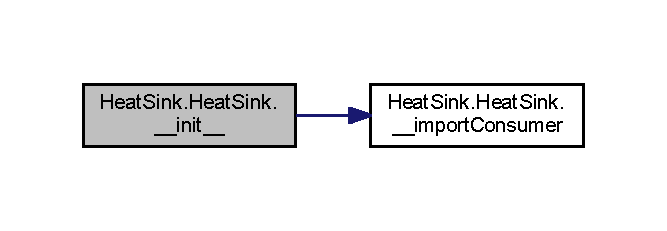
\includegraphics[width=320pt]{class_heat_sink_1_1_heat_sink_a1bd8a32977fa197c106013805bdedad7_cgraph}
\end{center}
\end{figure}


\subsection{Member Function Documentation}
\mbox{\Hypertarget{class_heat_sink_1_1_heat_sink_a10c8205c614c016c724f51c350b6ec18}\label{class_heat_sink_1_1_heat_sink_a10c8205c614c016c724f51c350b6ec18}} 
\index{Heat\+Sink\+::\+Heat\+Sink@{Heat\+Sink\+::\+Heat\+Sink}!consumer@{consumer}}
\index{consumer@{consumer}!Heat\+Sink\+::\+Heat\+Sink@{Heat\+Sink\+::\+Heat\+Sink}}
\subsubsection{\texorpdfstring{consumer()}{consumer()}}
{\footnotesize\ttfamily def Heat\+Sink.\+Heat\+Sink.\+consumer (\begin{DoxyParamCaption}\item[{}]{self,  }\item[{}]{i = {\ttfamily slice(None,None)} }\end{DoxyParamCaption})}



The documentation for this class was generated from the following file\+:\begin{DoxyCompactItemize}
\item 
C\+:/\+Users/jpelda/\+Documents/\+Git\+Hub/district\+Heating/class/\hyperlink{_heat_sink_8py}{Heat\+Sink.\+py}\end{DoxyCompactItemize}

\hypertarget{class_heat_sink___consumptionprofiles_1_1_heat_sink___consumptionprofiles}{}\section{Heat\+Sink\+\_\+\+Consumptionprofiles.\+Heat\+Sink\+\_\+\+Consumptionprofiles Class Reference}
\label{class_heat_sink___consumptionprofiles_1_1_heat_sink___consumptionprofiles}\index{Heat\+Sink\+\_\+\+Consumptionprofiles.\+Heat\+Sink\+\_\+\+Consumptionprofiles@{Heat\+Sink\+\_\+\+Consumptionprofiles.\+Heat\+Sink\+\_\+\+Consumptionprofiles}}
\subsection*{Public Member Functions}
\begin{DoxyCompactItemize}
\item 
def \hyperlink{class_heat_sink___consumptionprofiles_1_1_heat_sink___consumptionprofiles_a0a98cfa6bb822aecb7b5b1f977def1f8}{\+\_\+\+\_\+init\+\_\+\+\_\+}
\item 
def \hyperlink{class_heat_sink___consumptionprofiles_1_1_heat_sink___consumptionprofiles_a5e52056f8f430a2aa642948af5246a2f}{date} (self, i=slice(None, None))
\item 
def \hyperlink{class_heat_sink___consumptionprofiles_1_1_heat_sink___consumptionprofiles_a62866d4ad34ff5cd3128356fd4996931}{consumption\+Profile} (self, profile, i=slice(None, None))
\end{DoxyCompactItemize}


\subsection{Constructor \& Destructor Documentation}
\mbox{\Hypertarget{class_heat_sink___consumptionprofiles_1_1_heat_sink___consumptionprofiles_a0a98cfa6bb822aecb7b5b1f977def1f8}\label{class_heat_sink___consumptionprofiles_1_1_heat_sink___consumptionprofiles_a0a98cfa6bb822aecb7b5b1f977def1f8}} 
\index{Heat\+Sink\+\_\+\+Consumptionprofiles\+::\+Heat\+Sink\+\_\+\+Consumptionprofiles@{Heat\+Sink\+\_\+\+Consumptionprofiles\+::\+Heat\+Sink\+\_\+\+Consumptionprofiles}!\+\_\+\+\_\+init\+\_\+\+\_\+@{\+\_\+\+\_\+init\+\_\+\+\_\+}}
\index{\+\_\+\+\_\+init\+\_\+\+\_\+@{\+\_\+\+\_\+init\+\_\+\+\_\+}!Heat\+Sink\+\_\+\+Consumptionprofiles\+::\+Heat\+Sink\+\_\+\+Consumptionprofiles@{Heat\+Sink\+\_\+\+Consumptionprofiles\+::\+Heat\+Sink\+\_\+\+Consumptionprofiles}}
\subsubsection{\texorpdfstring{\+\_\+\+\_\+init\+\_\+\+\_\+()}{\_\_init\_\_()}}
{\footnotesize\ttfamily def Heat\+Sink\+\_\+\+Consumptionprofiles.\+Heat\+Sink\+\_\+\+Consumptionprofiles.\+\_\+\+\_\+init\+\_\+\+\_\+ (\begin{DoxyParamCaption}\item[{}]{self,  }\item[{}]{filename = {\ttfamily os.getcwd()~+~os.sep~+~\textquotesingle{}heat\+\_\+consumptionProfiles.csv\textquotesingle{}},  }\item[{}]{startrow = {\ttfamily 1},  }\item[{}]{dtype = {\ttfamily \{\textquotesingle{}names\textquotesingle{}\+:(
~~~~~~~~~~~~~~~~~~~~~~~~~~~~~~~~\textquotesingle{}\hyperlink{class_heat_sink___consumptionprofiles_1_1_heat_sink___consumptionprofiles_a5e52056f8f430a2aa642948af5246a2f}{date}\textquotesingle{},
~~~~~~~~~~~~~~~~~~~~~~~~~~~~~~~~\textquotesingle{}house\textquotesingle{},
~~~~~~~~~~~~~~~~~~~~~~~~~~~~~~~~\textquotesingle{}industry\textquotesingle{},
~~~~~~~~~~~~~~~~~~~~~~~~~~~~~~~~)},  }\item[{}]{formats }\end{DoxyParamCaption})}



\subsection{Member Function Documentation}
\mbox{\Hypertarget{class_heat_sink___consumptionprofiles_1_1_heat_sink___consumptionprofiles_a62866d4ad34ff5cd3128356fd4996931}\label{class_heat_sink___consumptionprofiles_1_1_heat_sink___consumptionprofiles_a62866d4ad34ff5cd3128356fd4996931}} 
\index{Heat\+Sink\+\_\+\+Consumptionprofiles\+::\+Heat\+Sink\+\_\+\+Consumptionprofiles@{Heat\+Sink\+\_\+\+Consumptionprofiles\+::\+Heat\+Sink\+\_\+\+Consumptionprofiles}!consumption\+Profile@{consumption\+Profile}}
\index{consumption\+Profile@{consumption\+Profile}!Heat\+Sink\+\_\+\+Consumptionprofiles\+::\+Heat\+Sink\+\_\+\+Consumptionprofiles@{Heat\+Sink\+\_\+\+Consumptionprofiles\+::\+Heat\+Sink\+\_\+\+Consumptionprofiles}}
\subsubsection{\texorpdfstring{consumption\+Profile()}{consumptionProfile()}}
{\footnotesize\ttfamily def Heat\+Sink\+\_\+\+Consumptionprofiles.\+Heat\+Sink\+\_\+\+Consumptionprofiles.\+consumption\+Profile (\begin{DoxyParamCaption}\item[{}]{self,  }\item[{}]{profile,  }\item[{}]{i = {\ttfamily slice(None,None)} }\end{DoxyParamCaption})}

\mbox{\Hypertarget{class_heat_sink___consumptionprofiles_1_1_heat_sink___consumptionprofiles_a5e52056f8f430a2aa642948af5246a2f}\label{class_heat_sink___consumptionprofiles_1_1_heat_sink___consumptionprofiles_a5e52056f8f430a2aa642948af5246a2f}} 
\index{Heat\+Sink\+\_\+\+Consumptionprofiles\+::\+Heat\+Sink\+\_\+\+Consumptionprofiles@{Heat\+Sink\+\_\+\+Consumptionprofiles\+::\+Heat\+Sink\+\_\+\+Consumptionprofiles}!date@{date}}
\index{date@{date}!Heat\+Sink\+\_\+\+Consumptionprofiles\+::\+Heat\+Sink\+\_\+\+Consumptionprofiles@{Heat\+Sink\+\_\+\+Consumptionprofiles\+::\+Heat\+Sink\+\_\+\+Consumptionprofiles}}
\subsubsection{\texorpdfstring{date()}{date()}}
{\footnotesize\ttfamily def Heat\+Sink\+\_\+\+Consumptionprofiles.\+Heat\+Sink\+\_\+\+Consumptionprofiles.\+date (\begin{DoxyParamCaption}\item[{}]{self,  }\item[{}]{i = {\ttfamily slice(None,None)} }\end{DoxyParamCaption})}



The documentation for this class was generated from the following file\+:\begin{DoxyCompactItemize}
\item 
C\+:/\+Users/jpelda/\+Documents/\+Git\+Hub/district\+Heating/class/\hyperlink{_heat_sink___consumptionprofiles_8py}{Heat\+Sink\+\_\+\+Consumptionprofiles.\+py}\end{DoxyCompactItemize}

\hypertarget{class_heat_source_1_1_heat_source}{}\section{Heat\+Source.\+Heat\+Source Class Reference}
\label{class_heat_source_1_1_heat_source}\index{Heat\+Source.\+Heat\+Source@{Heat\+Source.\+Heat\+Source}}
\subsection*{Public Member Functions}
\begin{DoxyCompactItemize}
\item 
def \hyperlink{class_heat_source_1_1_heat_source_a0aa3ba858e7b64f2a0a3a27d91714097}{\+\_\+\+\_\+init\+\_\+\+\_\+} (self, table\+Of\+Producer)
\item 
def \hyperlink{class_heat_source_1_1_heat_source_a2c86ea2252b3a4f0eec9428fc61e14ab}{producer} (self, i=slice(None, None))
\end{DoxyCompactItemize}


\subsection{Constructor \& Destructor Documentation}
\mbox{\Hypertarget{class_heat_source_1_1_heat_source_a0aa3ba858e7b64f2a0a3a27d91714097}\label{class_heat_source_1_1_heat_source_a0aa3ba858e7b64f2a0a3a27d91714097}} 
\index{Heat\+Source\+::\+Heat\+Source@{Heat\+Source\+::\+Heat\+Source}!\+\_\+\+\_\+init\+\_\+\+\_\+@{\+\_\+\+\_\+init\+\_\+\+\_\+}}
\index{\+\_\+\+\_\+init\+\_\+\+\_\+@{\+\_\+\+\_\+init\+\_\+\+\_\+}!Heat\+Source\+::\+Heat\+Source@{Heat\+Source\+::\+Heat\+Source}}
\subsubsection{\texorpdfstring{\+\_\+\+\_\+init\+\_\+\+\_\+()}{\_\_init\_\_()}}
{\footnotesize\ttfamily def Heat\+Source.\+Heat\+Source.\+\_\+\+\_\+init\+\_\+\+\_\+ (\begin{DoxyParamCaption}\item[{}]{self,  }\item[{}]{table\+Of\+Producer }\end{DoxyParamCaption})}

Here is the call graph for this function\+:
\nopagebreak
\begin{figure}[H]
\begin{center}
\leavevmode
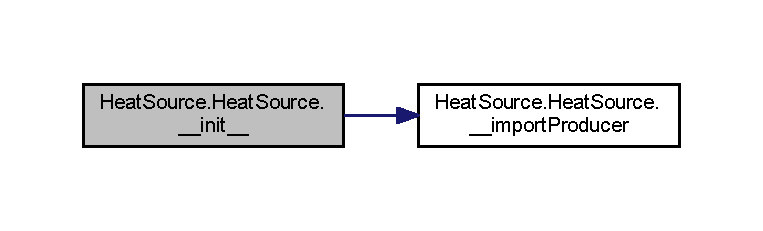
\includegraphics[width=350pt]{class_heat_source_1_1_heat_source_a0aa3ba858e7b64f2a0a3a27d91714097_cgraph}
\end{center}
\end{figure}


\subsection{Member Function Documentation}
\mbox{\Hypertarget{class_heat_source_1_1_heat_source_a2c86ea2252b3a4f0eec9428fc61e14ab}\label{class_heat_source_1_1_heat_source_a2c86ea2252b3a4f0eec9428fc61e14ab}} 
\index{Heat\+Source\+::\+Heat\+Source@{Heat\+Source\+::\+Heat\+Source}!producer@{producer}}
\index{producer@{producer}!Heat\+Source\+::\+Heat\+Source@{Heat\+Source\+::\+Heat\+Source}}
\subsubsection{\texorpdfstring{producer()}{producer()}}
{\footnotesize\ttfamily def Heat\+Source.\+Heat\+Source.\+producer (\begin{DoxyParamCaption}\item[{}]{self,  }\item[{}]{i = {\ttfamily slice(None,None)} }\end{DoxyParamCaption})}



The documentation for this class was generated from the following file\+:\begin{DoxyCompactItemize}
\item 
C\+:/\+Users/jpelda/\+Documents/\+Git\+Hub/district\+Heating/class/\hyperlink{_heat_source_8py}{Heat\+Source.\+py}\end{DoxyCompactItemize}

\hypertarget{class_node_1_1_node}{}\section{Node.\+Node Class Reference}
\label{class_node_1_1_node}\index{Node.\+Node@{Node.\+Node}}
\subsection*{Public Member Functions}
\begin{DoxyCompactItemize}
\item 
def \hyperlink{class_node_1_1_node_a07eea18e16b4ea130ed202d99512091b}{\+\_\+\+\_\+init\+\_\+\+\_\+} (self, node\+Values)
\end{DoxyCompactItemize}
\subsection*{Public Attributes}
\begin{DoxyCompactItemize}
\item 
\hyperlink{class_node_1_1_node_aef9465565b12f9f28b6aefe822948af5}{index}
\item 
\hyperlink{class_node_1_1_node_a6bfcdef2c07be856e8850fcbdbb82025}{x}
\item 
\hyperlink{class_node_1_1_node_aab9b32354c529afe23970aeda52308b9}{y}
\item 
\hyperlink{class_node_1_1_node_a66728b66d1a530a57277759e3993550c}{name}
\item 
\hyperlink{class_node_1_1_node_aca249f2f0b0bcb239c4e201048412b72}{height}
\item 
\hyperlink{class_node_1_1_node_a036a86db86d1899d2dff6915f6092328}{S\+P\+\_\+\+RP}
\end{DoxyCompactItemize}


\subsection{Detailed Description}


Definition at line 9 of file Node.\+py.



\subsection{Constructor \& Destructor Documentation}
\mbox{\Hypertarget{class_node_1_1_node_a07eea18e16b4ea130ed202d99512091b}\label{class_node_1_1_node_a07eea18e16b4ea130ed202d99512091b}} 
\index{Node\+::\+Node@{Node\+::\+Node}!\+\_\+\+\_\+init\+\_\+\+\_\+@{\+\_\+\+\_\+init\+\_\+\+\_\+}}
\index{\+\_\+\+\_\+init\+\_\+\+\_\+@{\+\_\+\+\_\+init\+\_\+\+\_\+}!Node\+::\+Node@{Node\+::\+Node}}
\subsubsection{\texorpdfstring{\+\_\+\+\_\+init\+\_\+\+\_\+()}{\_\_init\_\_()}}
{\footnotesize\ttfamily def Node.\+Node.\+\_\+\+\_\+init\+\_\+\+\_\+ (\begin{DoxyParamCaption}\item[{}]{self,  }\item[{}]{node\+Values }\end{DoxyParamCaption})}



Definition at line 10 of file Node.\+py.



\subsection{Member Data Documentation}
\mbox{\Hypertarget{class_node_1_1_node_aca249f2f0b0bcb239c4e201048412b72}\label{class_node_1_1_node_aca249f2f0b0bcb239c4e201048412b72}} 
\index{Node\+::\+Node@{Node\+::\+Node}!height@{height}}
\index{height@{height}!Node\+::\+Node@{Node\+::\+Node}}
\subsubsection{\texorpdfstring{height}{height}}
{\footnotesize\ttfamily Node.\+Node.\+height}



Definition at line 15 of file Node.\+py.

\mbox{\Hypertarget{class_node_1_1_node_aef9465565b12f9f28b6aefe822948af5}\label{class_node_1_1_node_aef9465565b12f9f28b6aefe822948af5}} 
\index{Node\+::\+Node@{Node\+::\+Node}!index@{index}}
\index{index@{index}!Node\+::\+Node@{Node\+::\+Node}}
\subsubsection{\texorpdfstring{index}{index}}
{\footnotesize\ttfamily Node.\+Node.\+index}



Definition at line 11 of file Node.\+py.

\mbox{\Hypertarget{class_node_1_1_node_a66728b66d1a530a57277759e3993550c}\label{class_node_1_1_node_a66728b66d1a530a57277759e3993550c}} 
\index{Node\+::\+Node@{Node\+::\+Node}!name@{name}}
\index{name@{name}!Node\+::\+Node@{Node\+::\+Node}}
\subsubsection{\texorpdfstring{name}{name}}
{\footnotesize\ttfamily Node.\+Node.\+name}



Definition at line 14 of file Node.\+py.

\mbox{\Hypertarget{class_node_1_1_node_a036a86db86d1899d2dff6915f6092328}\label{class_node_1_1_node_a036a86db86d1899d2dff6915f6092328}} 
\index{Node\+::\+Node@{Node\+::\+Node}!S\+P\+\_\+\+RP@{S\+P\+\_\+\+RP}}
\index{S\+P\+\_\+\+RP@{S\+P\+\_\+\+RP}!Node\+::\+Node@{Node\+::\+Node}}
\subsubsection{\texorpdfstring{S\+P\+\_\+\+RP}{SP\_RP}}
{\footnotesize\ttfamily Node.\+Node.\+S\+P\+\_\+\+RP}



Definition at line 16 of file Node.\+py.

\mbox{\Hypertarget{class_node_1_1_node_a6bfcdef2c07be856e8850fcbdbb82025}\label{class_node_1_1_node_a6bfcdef2c07be856e8850fcbdbb82025}} 
\index{Node\+::\+Node@{Node\+::\+Node}!x@{x}}
\index{x@{x}!Node\+::\+Node@{Node\+::\+Node}}
\subsubsection{\texorpdfstring{x}{x}}
{\footnotesize\ttfamily Node.\+Node.\+x}



Definition at line 12 of file Node.\+py.

\mbox{\Hypertarget{class_node_1_1_node_aab9b32354c529afe23970aeda52308b9}\label{class_node_1_1_node_aab9b32354c529afe23970aeda52308b9}} 
\index{Node\+::\+Node@{Node\+::\+Node}!y@{y}}
\index{y@{y}!Node\+::\+Node@{Node\+::\+Node}}
\subsubsection{\texorpdfstring{y}{y}}
{\footnotesize\ttfamily Node.\+Node.\+y}



Definition at line 13 of file Node.\+py.



The documentation for this class was generated from the following file\+:\begin{DoxyCompactItemize}
\item 
C\+:/\+Users/jpelda/\+Documents/\+Git\+Hub/district\+Heating/class/\hyperlink{_node_8py}{Node.\+py}\end{DoxyCompactItemize}

\hypertarget{class_pipe_1_1_pipe}{}\section{Pipe.\+Pipe Class Reference}
\label{class_pipe_1_1_pipe}\index{Pipe.\+Pipe@{Pipe.\+Pipe}}
\subsection*{Public Member Functions}
\begin{DoxyCompactItemize}
\item 
def \hyperlink{class_pipe_1_1_pipe_af59d40a027d25c62e41d11a08f14729f}{\+\_\+\+\_\+init\+\_\+\+\_\+} (self, pipe\+Values)
\item 
def \hyperlink{class_pipe_1_1_pipe_a628661bc972aee1bc2f84623fcfaed91}{set\+Heatflow} (self, heat\+Flow)
\item 
def \hyperlink{class_pipe_1_1_pipe_afbd372f6badcea91558e723eb0c81712}{get\+Heatflow} (self)
\item 
def \hyperlink{class_pipe_1_1_pipe_a184f926c3aee89e94c19b003d6cc9416}{start\+\_\+flowspeed} (self)
\item 
def \hyperlink{class_pipe_1_1_pipe_afec35167b5ad4acf26ea2db36292d135}{reynold} (self)
\item 
def \hyperlink{class_pipe_1_1_pipe_a6cda251ee7a5bb112b2dbe8db6a76448}{heat\+\_\+transfer\+Coefficient} (self, transfer\+Coefficients, layer\+\_\+heat\+\_\+conductivities, layer\+\_\+thicknesses)
\item 
def \hyperlink{class_pipe_1_1_pipe_a51bf5b3d3334c008e8cb92c8e8e2e9d1}{heatloss} (self)
\item 
def \hyperlink{class_pipe_1_1_pipe_aa09f88a2a098f433547773dcee75da6c}{pipe\+\_\+lambda} (self)
\item 
def \hyperlink{class_pipe_1_1_pipe_a69d6c5c5204633f84cc45801adf17aed}{pressure\+\_\+difference} (self)
\item 
def \hyperlink{class_pipe_1_1_pipe_a93aa9c0dd790f2014d2c403b23164646}{end\+\_\+pressure} (self, start\+\_\+pressure)
\item 
def \hyperlink{class_pipe_1_1_pipe_ae2b6ac79c8416e15bb8846739e90d0f6}{end\+\_\+volume\+Stream} (self)
\item 
def \hyperlink{class_pipe_1_1_pipe_abab09825864d4997d16ffc1dcdbfcf97}{end\+\_\+flowspeed} (self)
\item 
def \hyperlink{class_pipe_1_1_pipe_a2fdfff20143b09a5c32f335bf55edebc}{volume} (self)
\end{DoxyCompactItemize}
\subsection*{Public Attributes}
\begin{DoxyCompactItemize}
\item 
\hyperlink{class_pipe_1_1_pipe_a721626d39e9fa569ff1bea20d43d6891}{ambient\+\_\+temp}
\item 
\hyperlink{class_pipe_1_1_pipe_a9ac4eaff0763b3dffd827858c02166bd}{fluid\+\_\+temp}
\item 
\hyperlink{class_pipe_1_1_pipe_a1fb5c94ac5e6dac7b415a170524a75f5}{index}
\item 
\hyperlink{class_pipe_1_1_pipe_a99b713a0d71ea921e5fdd7665a294598}{start\+\_\+x}
\item 
\hyperlink{class_pipe_1_1_pipe_a9104dacc2e9f3541a8171c7d7bbf8a2e}{start\+\_\+y}
\item 
\hyperlink{class_pipe_1_1_pipe_a3c89ac40d76fd166fb08ebb585ef220e}{end\+\_\+x}
\item 
\hyperlink{class_pipe_1_1_pipe_a8ea1c50334527d53a3c83b26f2c41dfa}{end\+\_\+y}
\item 
\hyperlink{class_pipe_1_1_pipe_ad604bcf622bea20a2e6089515e793700}{start\+\_\+node\+\_\+name}
\item 
\hyperlink{class_pipe_1_1_pipe_ae09a8821336f622e4215d22bdead0952}{end\+\_\+node\+\_\+name}
\item 
\hyperlink{class_pipe_1_1_pipe_aed39cdfd26dab2d8aa176fbcc8ee0eac}{length}
\item 
\hyperlink{class_pipe_1_1_pipe_a498f8ef080ca2ef5533d4bb239c02e84}{diameter\+\_\+inner}
\item 
\hyperlink{class_pipe_1_1_pipe_ad4a6c940a7986e70a34f4d7dc5659a19}{diameter\+\_\+outer}
\item 
\hyperlink{class_pipe_1_1_pipe_acdfc6a6bdd70105a3342553a03ad9277}{start\+\_\+height}
\item 
\hyperlink{class_pipe_1_1_pipe_a8c66a7b6c464b5c48d567c19be7e72ca}{end\+\_\+height}
\item 
\hyperlink{class_pipe_1_1_pipe_ae5cec5540b37294ed43fad9d9f187d4b}{roughness}
\item 
\hyperlink{class_pipe_1_1_pipe_a94e84282ca30ec24343eb219f67e783b}{S\+P\+\_\+\+RP}
\item 
\hyperlink{class_pipe_1_1_pipe_ad75af1651b56fe12e4cff8d1254afa98}{heat\+Transition\+Coefficient}
\end{DoxyCompactItemize}


\subsection{Detailed Description}


Definition at line 12 of file Pipe.\+py.



\subsection{Constructor \& Destructor Documentation}
\mbox{\Hypertarget{class_pipe_1_1_pipe_af59d40a027d25c62e41d11a08f14729f}\label{class_pipe_1_1_pipe_af59d40a027d25c62e41d11a08f14729f}} 
\index{Pipe\+::\+Pipe@{Pipe\+::\+Pipe}!\+\_\+\+\_\+init\+\_\+\+\_\+@{\+\_\+\+\_\+init\+\_\+\+\_\+}}
\index{\+\_\+\+\_\+init\+\_\+\+\_\+@{\+\_\+\+\_\+init\+\_\+\+\_\+}!Pipe\+::\+Pipe@{Pipe\+::\+Pipe}}
\subsubsection{\texorpdfstring{\+\_\+\+\_\+init\+\_\+\+\_\+()}{\_\_init\_\_()}}
{\footnotesize\ttfamily def Pipe.\+Pipe.\+\_\+\+\_\+init\+\_\+\+\_\+ (\begin{DoxyParamCaption}\item[{}]{self,  }\item[{}]{pipe\+Values }\end{DoxyParamCaption})}



Definition at line 13 of file Pipe.\+py.



\subsection{Member Function Documentation}
\mbox{\Hypertarget{class_pipe_1_1_pipe_abab09825864d4997d16ffc1dcdbfcf97}\label{class_pipe_1_1_pipe_abab09825864d4997d16ffc1dcdbfcf97}} 
\index{Pipe\+::\+Pipe@{Pipe\+::\+Pipe}!end\+\_\+flowspeed@{end\+\_\+flowspeed}}
\index{end\+\_\+flowspeed@{end\+\_\+flowspeed}!Pipe\+::\+Pipe@{Pipe\+::\+Pipe}}
\subsubsection{\texorpdfstring{end\+\_\+flowspeed()}{end\_flowspeed()}}
{\footnotesize\ttfamily def Pipe.\+Pipe.\+end\+\_\+flowspeed (\begin{DoxyParamCaption}\item[{}]{self }\end{DoxyParamCaption})}



Definition at line 209 of file Pipe.\+py.

\mbox{\Hypertarget{class_pipe_1_1_pipe_a93aa9c0dd790f2014d2c403b23164646}\label{class_pipe_1_1_pipe_a93aa9c0dd790f2014d2c403b23164646}} 
\index{Pipe\+::\+Pipe@{Pipe\+::\+Pipe}!end\+\_\+pressure@{end\+\_\+pressure}}
\index{end\+\_\+pressure@{end\+\_\+pressure}!Pipe\+::\+Pipe@{Pipe\+::\+Pipe}}
\subsubsection{\texorpdfstring{end\+\_\+pressure()}{end\_pressure()}}
{\footnotesize\ttfamily def Pipe.\+Pipe.\+end\+\_\+pressure (\begin{DoxyParamCaption}\item[{}]{self,  }\item[{}]{start\+\_\+pressure }\end{DoxyParamCaption})}



Definition at line 200 of file Pipe.\+py.

\mbox{\Hypertarget{class_pipe_1_1_pipe_ae2b6ac79c8416e15bb8846739e90d0f6}\label{class_pipe_1_1_pipe_ae2b6ac79c8416e15bb8846739e90d0f6}} 
\index{Pipe\+::\+Pipe@{Pipe\+::\+Pipe}!end\+\_\+volume\+Stream@{end\+\_\+volume\+Stream}}
\index{end\+\_\+volume\+Stream@{end\+\_\+volume\+Stream}!Pipe\+::\+Pipe@{Pipe\+::\+Pipe}}
\subsubsection{\texorpdfstring{end\+\_\+volume\+Stream()}{end\_volumeStream()}}
{\footnotesize\ttfamily def Pipe.\+Pipe.\+end\+\_\+volume\+Stream (\begin{DoxyParamCaption}\item[{}]{self }\end{DoxyParamCaption})}



Definition at line 204 of file Pipe.\+py.

\mbox{\Hypertarget{class_pipe_1_1_pipe_afbd372f6badcea91558e723eb0c81712}\label{class_pipe_1_1_pipe_afbd372f6badcea91558e723eb0c81712}} 
\index{Pipe\+::\+Pipe@{Pipe\+::\+Pipe}!get\+Heatflow@{get\+Heatflow}}
\index{get\+Heatflow@{get\+Heatflow}!Pipe\+::\+Pipe@{Pipe\+::\+Pipe}}
\subsubsection{\texorpdfstring{get\+Heatflow()}{getHeatflow()}}
{\footnotesize\ttfamily def Pipe.\+Pipe.\+get\+Heatflow (\begin{DoxyParamCaption}\item[{}]{self }\end{DoxyParamCaption})}



Definition at line 81 of file Pipe.\+py.

\mbox{\Hypertarget{class_pipe_1_1_pipe_a6cda251ee7a5bb112b2dbe8db6a76448}\label{class_pipe_1_1_pipe_a6cda251ee7a5bb112b2dbe8db6a76448}} 
\index{Pipe\+::\+Pipe@{Pipe\+::\+Pipe}!heat\+\_\+transfer\+Coefficient@{heat\+\_\+transfer\+Coefficient}}
\index{heat\+\_\+transfer\+Coefficient@{heat\+\_\+transfer\+Coefficient}!Pipe\+::\+Pipe@{Pipe\+::\+Pipe}}
\subsubsection{\texorpdfstring{heat\+\_\+transfer\+Coefficient()}{heat\_transferCoefficient()}}
{\footnotesize\ttfamily def Pipe.\+Pipe.\+heat\+\_\+transfer\+Coefficient (\begin{DoxyParamCaption}\item[{}]{self,  }\item[{}]{transfer\+Coefficients,  }\item[{}]{layer\+\_\+heat\+\_\+conductivities,  }\item[{}]{layer\+\_\+thicknesses }\end{DoxyParamCaption})}

\begin{DoxyVerb}array of transferCoefficients = alpha [W / m²*K]
array of heat_conductivities = lamda [W / m*K]
\end{DoxyVerb}
 

Definition at line 114 of file Pipe.\+py.

\mbox{\Hypertarget{class_pipe_1_1_pipe_a51bf5b3d3334c008e8cb92c8e8e2e9d1}\label{class_pipe_1_1_pipe_a51bf5b3d3334c008e8cb92c8e8e2e9d1}} 
\index{Pipe\+::\+Pipe@{Pipe\+::\+Pipe}!heatloss@{heatloss}}
\index{heatloss@{heatloss}!Pipe\+::\+Pipe@{Pipe\+::\+Pipe}}
\subsubsection{\texorpdfstring{heatloss()}{heatloss()}}
{\footnotesize\ttfamily def Pipe.\+Pipe.\+heatloss (\begin{DoxyParamCaption}\item[{}]{self }\end{DoxyParamCaption})}



Definition at line 126 of file Pipe.\+py.

\mbox{\Hypertarget{class_pipe_1_1_pipe_aa09f88a2a098f433547773dcee75da6c}\label{class_pipe_1_1_pipe_aa09f88a2a098f433547773dcee75da6c}} 
\index{Pipe\+::\+Pipe@{Pipe\+::\+Pipe}!pipe\+\_\+lambda@{pipe\+\_\+lambda}}
\index{pipe\+\_\+lambda@{pipe\+\_\+lambda}!Pipe\+::\+Pipe@{Pipe\+::\+Pipe}}
\subsubsection{\texorpdfstring{pipe\+\_\+lambda()}{pipe\_lambda()}}
{\footnotesize\ttfamily def Pipe.\+Pipe.\+pipe\+\_\+lambda (\begin{DoxyParamCaption}\item[{}]{self }\end{DoxyParamCaption})}

\begin{DoxyVerb}Calculation of lambda
If the flow is laminar...
else if the flow is turbulent...
\end{DoxyVerb}
 

Definition at line 153 of file Pipe.\+py.

\mbox{\Hypertarget{class_pipe_1_1_pipe_a69d6c5c5204633f84cc45801adf17aed}\label{class_pipe_1_1_pipe_a69d6c5c5204633f84cc45801adf17aed}} 
\index{Pipe\+::\+Pipe@{Pipe\+::\+Pipe}!pressure\+\_\+difference@{pressure\+\_\+difference}}
\index{pressure\+\_\+difference@{pressure\+\_\+difference}!Pipe\+::\+Pipe@{Pipe\+::\+Pipe}}
\subsubsection{\texorpdfstring{pressure\+\_\+difference()}{pressure\_difference()}}
{\footnotesize\ttfamily def Pipe.\+Pipe.\+pressure\+\_\+difference (\begin{DoxyParamCaption}\item[{}]{self }\end{DoxyParamCaption})}

\begin{DoxyVerb}Difference between PressureStart and PressureEnd
calculated by Darcy-Law
\end{DoxyVerb}
 

Definition at line 184 of file Pipe.\+py.

\mbox{\Hypertarget{class_pipe_1_1_pipe_afec35167b5ad4acf26ea2db36292d135}\label{class_pipe_1_1_pipe_afec35167b5ad4acf26ea2db36292d135}} 
\index{Pipe\+::\+Pipe@{Pipe\+::\+Pipe}!reynold@{reynold}}
\index{reynold@{reynold}!Pipe\+::\+Pipe@{Pipe\+::\+Pipe}}
\subsubsection{\texorpdfstring{reynold()}{reynold()}}
{\footnotesize\ttfamily def Pipe.\+Pipe.\+reynold (\begin{DoxyParamCaption}\item[{}]{self }\end{DoxyParamCaption})}

\begin{DoxyVerb}calculation of reynold number

Re = (w * d) / kinvis
\end{DoxyVerb}
 

Definition at line 100 of file Pipe.\+py.

\mbox{\Hypertarget{class_pipe_1_1_pipe_a628661bc972aee1bc2f84623fcfaed91}\label{class_pipe_1_1_pipe_a628661bc972aee1bc2f84623fcfaed91}} 
\index{Pipe\+::\+Pipe@{Pipe\+::\+Pipe}!set\+Heatflow@{set\+Heatflow}}
\index{set\+Heatflow@{set\+Heatflow}!Pipe\+::\+Pipe@{Pipe\+::\+Pipe}}
\subsubsection{\texorpdfstring{set\+Heatflow()}{setHeatflow()}}
{\footnotesize\ttfamily def Pipe.\+Pipe.\+set\+Heatflow (\begin{DoxyParamCaption}\item[{}]{self,  }\item[{}]{heat\+Flow }\end{DoxyParamCaption})}



Definition at line 78 of file Pipe.\+py.

\mbox{\Hypertarget{class_pipe_1_1_pipe_a184f926c3aee89e94c19b003d6cc9416}\label{class_pipe_1_1_pipe_a184f926c3aee89e94c19b003d6cc9416}} 
\index{Pipe\+::\+Pipe@{Pipe\+::\+Pipe}!start\+\_\+flowspeed@{start\+\_\+flowspeed}}
\index{start\+\_\+flowspeed@{start\+\_\+flowspeed}!Pipe\+::\+Pipe@{Pipe\+::\+Pipe}}
\subsubsection{\texorpdfstring{start\+\_\+flowspeed()}{start\_flowspeed()}}
{\footnotesize\ttfamily def Pipe.\+Pipe.\+start\+\_\+flowspeed (\begin{DoxyParamCaption}\item[{}]{self }\end{DoxyParamCaption})}

\begin{DoxyVerb}calculation of flow speed

((m^3)/h) / 3600 = ((m^3)/s)

w = VolumeStream (in (m^3)/s) / A (in m^2)
\end{DoxyVerb}
 

Definition at line 86 of file Pipe.\+py.

\mbox{\Hypertarget{class_pipe_1_1_pipe_a2fdfff20143b09a5c32f335bf55edebc}\label{class_pipe_1_1_pipe_a2fdfff20143b09a5c32f335bf55edebc}} 
\index{Pipe\+::\+Pipe@{Pipe\+::\+Pipe}!volume@{volume}}
\index{volume@{volume}!Pipe\+::\+Pipe@{Pipe\+::\+Pipe}}
\subsubsection{\texorpdfstring{volume()}{volume()}}
{\footnotesize\ttfamily def Pipe.\+Pipe.\+volume (\begin{DoxyParamCaption}\item[{}]{self }\end{DoxyParamCaption})}



Definition at line 214 of file Pipe.\+py.



\subsection{Member Data Documentation}
\mbox{\Hypertarget{class_pipe_1_1_pipe_a721626d39e9fa569ff1bea20d43d6891}\label{class_pipe_1_1_pipe_a721626d39e9fa569ff1bea20d43d6891}} 
\index{Pipe\+::\+Pipe@{Pipe\+::\+Pipe}!ambient\+\_\+temp@{ambient\+\_\+temp}}
\index{ambient\+\_\+temp@{ambient\+\_\+temp}!Pipe\+::\+Pipe@{Pipe\+::\+Pipe}}
\subsubsection{\texorpdfstring{ambient\+\_\+temp}{ambient\_temp}}
{\footnotesize\ttfamily Pipe.\+Pipe.\+ambient\+\_\+temp}



Definition at line 15 of file Pipe.\+py.

\mbox{\Hypertarget{class_pipe_1_1_pipe_a498f8ef080ca2ef5533d4bb239c02e84}\label{class_pipe_1_1_pipe_a498f8ef080ca2ef5533d4bb239c02e84}} 
\index{Pipe\+::\+Pipe@{Pipe\+::\+Pipe}!diameter\+\_\+inner@{diameter\+\_\+inner}}
\index{diameter\+\_\+inner@{diameter\+\_\+inner}!Pipe\+::\+Pipe@{Pipe\+::\+Pipe}}
\subsubsection{\texorpdfstring{diameter\+\_\+inner}{diameter\_inner}}
{\footnotesize\ttfamily Pipe.\+Pipe.\+diameter\+\_\+inner}



Definition at line 35 of file Pipe.\+py.

\mbox{\Hypertarget{class_pipe_1_1_pipe_ad4a6c940a7986e70a34f4d7dc5659a19}\label{class_pipe_1_1_pipe_ad4a6c940a7986e70a34f4d7dc5659a19}} 
\index{Pipe\+::\+Pipe@{Pipe\+::\+Pipe}!diameter\+\_\+outer@{diameter\+\_\+outer}}
\index{diameter\+\_\+outer@{diameter\+\_\+outer}!Pipe\+::\+Pipe@{Pipe\+::\+Pipe}}
\subsubsection{\texorpdfstring{diameter\+\_\+outer}{diameter\_outer}}
{\footnotesize\ttfamily Pipe.\+Pipe.\+diameter\+\_\+outer}



Definition at line 36 of file Pipe.\+py.

\mbox{\Hypertarget{class_pipe_1_1_pipe_a8c66a7b6c464b5c48d567c19be7e72ca}\label{class_pipe_1_1_pipe_a8c66a7b6c464b5c48d567c19be7e72ca}} 
\index{Pipe\+::\+Pipe@{Pipe\+::\+Pipe}!end\+\_\+height@{end\+\_\+height}}
\index{end\+\_\+height@{end\+\_\+height}!Pipe\+::\+Pipe@{Pipe\+::\+Pipe}}
\subsubsection{\texorpdfstring{end\+\_\+height}{end\_height}}
{\footnotesize\ttfamily Pipe.\+Pipe.\+end\+\_\+height}



Definition at line 38 of file Pipe.\+py.

\mbox{\Hypertarget{class_pipe_1_1_pipe_ae09a8821336f622e4215d22bdead0952}\label{class_pipe_1_1_pipe_ae09a8821336f622e4215d22bdead0952}} 
\index{Pipe\+::\+Pipe@{Pipe\+::\+Pipe}!end\+\_\+node\+\_\+name@{end\+\_\+node\+\_\+name}}
\index{end\+\_\+node\+\_\+name@{end\+\_\+node\+\_\+name}!Pipe\+::\+Pipe@{Pipe\+::\+Pipe}}
\subsubsection{\texorpdfstring{end\+\_\+node\+\_\+name}{end\_node\_name}}
{\footnotesize\ttfamily Pipe.\+Pipe.\+end\+\_\+node\+\_\+name}



Definition at line 33 of file Pipe.\+py.

\mbox{\Hypertarget{class_pipe_1_1_pipe_a3c89ac40d76fd166fb08ebb585ef220e}\label{class_pipe_1_1_pipe_a3c89ac40d76fd166fb08ebb585ef220e}} 
\index{Pipe\+::\+Pipe@{Pipe\+::\+Pipe}!end\+\_\+x@{end\+\_\+x}}
\index{end\+\_\+x@{end\+\_\+x}!Pipe\+::\+Pipe@{Pipe\+::\+Pipe}}
\subsubsection{\texorpdfstring{end\+\_\+x}{end\_x}}
{\footnotesize\ttfamily Pipe.\+Pipe.\+end\+\_\+x}



Definition at line 30 of file Pipe.\+py.

\mbox{\Hypertarget{class_pipe_1_1_pipe_a8ea1c50334527d53a3c83b26f2c41dfa}\label{class_pipe_1_1_pipe_a8ea1c50334527d53a3c83b26f2c41dfa}} 
\index{Pipe\+::\+Pipe@{Pipe\+::\+Pipe}!end\+\_\+y@{end\+\_\+y}}
\index{end\+\_\+y@{end\+\_\+y}!Pipe\+::\+Pipe@{Pipe\+::\+Pipe}}
\subsubsection{\texorpdfstring{end\+\_\+y}{end\_y}}
{\footnotesize\ttfamily Pipe.\+Pipe.\+end\+\_\+y}



Definition at line 31 of file Pipe.\+py.

\mbox{\Hypertarget{class_pipe_1_1_pipe_a9ac4eaff0763b3dffd827858c02166bd}\label{class_pipe_1_1_pipe_a9ac4eaff0763b3dffd827858c02166bd}} 
\index{Pipe\+::\+Pipe@{Pipe\+::\+Pipe}!fluid\+\_\+temp@{fluid\+\_\+temp}}
\index{fluid\+\_\+temp@{fluid\+\_\+temp}!Pipe\+::\+Pipe@{Pipe\+::\+Pipe}}
\subsubsection{\texorpdfstring{fluid\+\_\+temp}{fluid\_temp}}
{\footnotesize\ttfamily Pipe.\+Pipe.\+fluid\+\_\+temp}



Definition at line 16 of file Pipe.\+py.

\mbox{\Hypertarget{class_pipe_1_1_pipe_ad75af1651b56fe12e4cff8d1254afa98}\label{class_pipe_1_1_pipe_ad75af1651b56fe12e4cff8d1254afa98}} 
\index{Pipe\+::\+Pipe@{Pipe\+::\+Pipe}!heat\+Transition\+Coefficient@{heat\+Transition\+Coefficient}}
\index{heat\+Transition\+Coefficient@{heat\+Transition\+Coefficient}!Pipe\+::\+Pipe@{Pipe\+::\+Pipe}}
\subsubsection{\texorpdfstring{heat\+Transition\+Coefficient}{heatTransitionCoefficient}}
{\footnotesize\ttfamily Pipe.\+Pipe.\+heat\+Transition\+Coefficient}



Definition at line 43 of file Pipe.\+py.

\mbox{\Hypertarget{class_pipe_1_1_pipe_a1fb5c94ac5e6dac7b415a170524a75f5}\label{class_pipe_1_1_pipe_a1fb5c94ac5e6dac7b415a170524a75f5}} 
\index{Pipe\+::\+Pipe@{Pipe\+::\+Pipe}!index@{index}}
\index{index@{index}!Pipe\+::\+Pipe@{Pipe\+::\+Pipe}}
\subsubsection{\texorpdfstring{index}{index}}
{\footnotesize\ttfamily Pipe.\+Pipe.\+index}



Definition at line 27 of file Pipe.\+py.

\mbox{\Hypertarget{class_pipe_1_1_pipe_aed39cdfd26dab2d8aa176fbcc8ee0eac}\label{class_pipe_1_1_pipe_aed39cdfd26dab2d8aa176fbcc8ee0eac}} 
\index{Pipe\+::\+Pipe@{Pipe\+::\+Pipe}!length@{length}}
\index{length@{length}!Pipe\+::\+Pipe@{Pipe\+::\+Pipe}}
\subsubsection{\texorpdfstring{length}{length}}
{\footnotesize\ttfamily Pipe.\+Pipe.\+length}



Definition at line 34 of file Pipe.\+py.

\mbox{\Hypertarget{class_pipe_1_1_pipe_ae5cec5540b37294ed43fad9d9f187d4b}\label{class_pipe_1_1_pipe_ae5cec5540b37294ed43fad9d9f187d4b}} 
\index{Pipe\+::\+Pipe@{Pipe\+::\+Pipe}!roughness@{roughness}}
\index{roughness@{roughness}!Pipe\+::\+Pipe@{Pipe\+::\+Pipe}}
\subsubsection{\texorpdfstring{roughness}{roughness}}
{\footnotesize\ttfamily Pipe.\+Pipe.\+roughness}



Definition at line 39 of file Pipe.\+py.

\mbox{\Hypertarget{class_pipe_1_1_pipe_a94e84282ca30ec24343eb219f67e783b}\label{class_pipe_1_1_pipe_a94e84282ca30ec24343eb219f67e783b}} 
\index{Pipe\+::\+Pipe@{Pipe\+::\+Pipe}!S\+P\+\_\+\+RP@{S\+P\+\_\+\+RP}}
\index{S\+P\+\_\+\+RP@{S\+P\+\_\+\+RP}!Pipe\+::\+Pipe@{Pipe\+::\+Pipe}}
\subsubsection{\texorpdfstring{S\+P\+\_\+\+RP}{SP\_RP}}
{\footnotesize\ttfamily Pipe.\+Pipe.\+S\+P\+\_\+\+RP}



Definition at line 40 of file Pipe.\+py.

\mbox{\Hypertarget{class_pipe_1_1_pipe_acdfc6a6bdd70105a3342553a03ad9277}\label{class_pipe_1_1_pipe_acdfc6a6bdd70105a3342553a03ad9277}} 
\index{Pipe\+::\+Pipe@{Pipe\+::\+Pipe}!start\+\_\+height@{start\+\_\+height}}
\index{start\+\_\+height@{start\+\_\+height}!Pipe\+::\+Pipe@{Pipe\+::\+Pipe}}
\subsubsection{\texorpdfstring{start\+\_\+height}{start\_height}}
{\footnotesize\ttfamily Pipe.\+Pipe.\+start\+\_\+height}



Definition at line 37 of file Pipe.\+py.

\mbox{\Hypertarget{class_pipe_1_1_pipe_ad604bcf622bea20a2e6089515e793700}\label{class_pipe_1_1_pipe_ad604bcf622bea20a2e6089515e793700}} 
\index{Pipe\+::\+Pipe@{Pipe\+::\+Pipe}!start\+\_\+node\+\_\+name@{start\+\_\+node\+\_\+name}}
\index{start\+\_\+node\+\_\+name@{start\+\_\+node\+\_\+name}!Pipe\+::\+Pipe@{Pipe\+::\+Pipe}}
\subsubsection{\texorpdfstring{start\+\_\+node\+\_\+name}{start\_node\_name}}
{\footnotesize\ttfamily Pipe.\+Pipe.\+start\+\_\+node\+\_\+name}



Definition at line 32 of file Pipe.\+py.

\mbox{\Hypertarget{class_pipe_1_1_pipe_a99b713a0d71ea921e5fdd7665a294598}\label{class_pipe_1_1_pipe_a99b713a0d71ea921e5fdd7665a294598}} 
\index{Pipe\+::\+Pipe@{Pipe\+::\+Pipe}!start\+\_\+x@{start\+\_\+x}}
\index{start\+\_\+x@{start\+\_\+x}!Pipe\+::\+Pipe@{Pipe\+::\+Pipe}}
\subsubsection{\texorpdfstring{start\+\_\+x}{start\_x}}
{\footnotesize\ttfamily Pipe.\+Pipe.\+start\+\_\+x}



Definition at line 28 of file Pipe.\+py.

\mbox{\Hypertarget{class_pipe_1_1_pipe_a9104dacc2e9f3541a8171c7d7bbf8a2e}\label{class_pipe_1_1_pipe_a9104dacc2e9f3541a8171c7d7bbf8a2e}} 
\index{Pipe\+::\+Pipe@{Pipe\+::\+Pipe}!start\+\_\+y@{start\+\_\+y}}
\index{start\+\_\+y@{start\+\_\+y}!Pipe\+::\+Pipe@{Pipe\+::\+Pipe}}
\subsubsection{\texorpdfstring{start\+\_\+y}{start\_y}}
{\footnotesize\ttfamily Pipe.\+Pipe.\+start\+\_\+y}



Definition at line 29 of file Pipe.\+py.



The documentation for this class was generated from the following file\+:\begin{DoxyCompactItemize}
\item 
C\+:/\+Users/jpelda/\+Documents/\+Git\+Hub/district\+Heating/class/\hyperlink{_pipe_8py}{Pipe.\+py}\end{DoxyCompactItemize}

\hypertarget{class_producer_1_1_producer}{}\section{Producer.\+Producer Class Reference}
\label{class_producer_1_1_producer}\index{Producer.\+Producer@{Producer.\+Producer}}
\subsection*{Public Member Functions}
\begin{DoxyCompactItemize}
\item 
def \hyperlink{class_producer_1_1_producer_a539019a9459d608c34054052cc95e968}{\+\_\+\+\_\+init\+\_\+\+\_\+} (self, producer\+Values)
\end{DoxyCompactItemize}
\subsection*{Public Attributes}
\begin{DoxyCompactItemize}
\item 
\hyperlink{class_producer_1_1_producer_ad67f942ec31acad8c3ce847c70303830}{name}
\item 
\hyperlink{class_producer_1_1_producer_aab72b0ca4a83c49bb24847a3c11ff990}{power}
\item 
\hyperlink{class_producer_1_1_producer_ac2dfdc8e4a892cf9ada2722051190045}{start\+\_\+node\+\_\+name}
\item 
\hyperlink{class_producer_1_1_producer_ad58b32a20ff969543efeb26ab92cc0c8}{end\+\_\+node\+\_\+name}
\end{DoxyCompactItemize}


\subsection{Detailed Description}


Definition at line 8 of file Producer.\+py.



\subsection{Constructor \& Destructor Documentation}
\mbox{\Hypertarget{class_producer_1_1_producer_a539019a9459d608c34054052cc95e968}\label{class_producer_1_1_producer_a539019a9459d608c34054052cc95e968}} 
\index{Producer\+::\+Producer@{Producer\+::\+Producer}!\+\_\+\+\_\+init\+\_\+\+\_\+@{\+\_\+\+\_\+init\+\_\+\+\_\+}}
\index{\+\_\+\+\_\+init\+\_\+\+\_\+@{\+\_\+\+\_\+init\+\_\+\+\_\+}!Producer\+::\+Producer@{Producer\+::\+Producer}}
\subsubsection{\texorpdfstring{\+\_\+\+\_\+init\+\_\+\+\_\+()}{\_\_init\_\_()}}
{\footnotesize\ttfamily def Producer.\+Producer.\+\_\+\+\_\+init\+\_\+\+\_\+ (\begin{DoxyParamCaption}\item[{}]{self,  }\item[{}]{producer\+Values }\end{DoxyParamCaption})}



Definition at line 9 of file Producer.\+py.



\subsection{Member Data Documentation}
\mbox{\Hypertarget{class_producer_1_1_producer_ad58b32a20ff969543efeb26ab92cc0c8}\label{class_producer_1_1_producer_ad58b32a20ff969543efeb26ab92cc0c8}} 
\index{Producer\+::\+Producer@{Producer\+::\+Producer}!end\+\_\+node\+\_\+name@{end\+\_\+node\+\_\+name}}
\index{end\+\_\+node\+\_\+name@{end\+\_\+node\+\_\+name}!Producer\+::\+Producer@{Producer\+::\+Producer}}
\subsubsection{\texorpdfstring{end\+\_\+node\+\_\+name}{end\_node\_name}}
{\footnotesize\ttfamily Producer.\+Producer.\+end\+\_\+node\+\_\+name}



Definition at line 14 of file Producer.\+py.

\mbox{\Hypertarget{class_producer_1_1_producer_ad67f942ec31acad8c3ce847c70303830}\label{class_producer_1_1_producer_ad67f942ec31acad8c3ce847c70303830}} 
\index{Producer\+::\+Producer@{Producer\+::\+Producer}!name@{name}}
\index{name@{name}!Producer\+::\+Producer@{Producer\+::\+Producer}}
\subsubsection{\texorpdfstring{name}{name}}
{\footnotesize\ttfamily Producer.\+Producer.\+name}



Definition at line 11 of file Producer.\+py.

\mbox{\Hypertarget{class_producer_1_1_producer_aab72b0ca4a83c49bb24847a3c11ff990}\label{class_producer_1_1_producer_aab72b0ca4a83c49bb24847a3c11ff990}} 
\index{Producer\+::\+Producer@{Producer\+::\+Producer}!power@{power}}
\index{power@{power}!Producer\+::\+Producer@{Producer\+::\+Producer}}
\subsubsection{\texorpdfstring{power}{power}}
{\footnotesize\ttfamily Producer.\+Producer.\+power}



Definition at line 12 of file Producer.\+py.

\mbox{\Hypertarget{class_producer_1_1_producer_ac2dfdc8e4a892cf9ada2722051190045}\label{class_producer_1_1_producer_ac2dfdc8e4a892cf9ada2722051190045}} 
\index{Producer\+::\+Producer@{Producer\+::\+Producer}!start\+\_\+node\+\_\+name@{start\+\_\+node\+\_\+name}}
\index{start\+\_\+node\+\_\+name@{start\+\_\+node\+\_\+name}!Producer\+::\+Producer@{Producer\+::\+Producer}}
\subsubsection{\texorpdfstring{start\+\_\+node\+\_\+name}{start\_node\_name}}
{\footnotesize\ttfamily Producer.\+Producer.\+start\+\_\+node\+\_\+name}



Definition at line 13 of file Producer.\+py.



The documentation for this class was generated from the following file\+:\begin{DoxyCompactItemize}
\item 
C\+:/\+Users/jpelda/\+Documents/\+Git\+Hub/district\+Heating/class/\hyperlink{_producer_8py}{Producer.\+py}\end{DoxyCompactItemize}

\hypertarget{class_pump_1_1_pump}{}\section{Pump.\+Pump Class Reference}
\label{class_pump_1_1_pump}\index{Pump.\+Pump@{Pump.\+Pump}}
\subsection*{Public Member Functions}
\begin{DoxyCompactItemize}
\item 
def \hyperlink{class_pump_1_1_pump_ad14459de937821f1a7da00d1bc441736}{\+\_\+\+\_\+init\+\_\+\+\_\+} (self, pump\+Values)
\end{DoxyCompactItemize}
\subsection*{Public Attributes}
\begin{DoxyCompactItemize}
\item 
\hyperlink{class_pump_1_1_pump_a4949cef4c42e9e9c5d4aafeabfba6713}{index}
\item 
\hyperlink{class_pump_1_1_pump_accd80242e8b18e06dd204bd713faa6eb}{profil}
\item 
\hyperlink{class_pump_1_1_pump_af8930a9eacd9a2dc69ee882b522c835d}{start\+\_\+node\+\_\+name}
\item 
\hyperlink{class_pump_1_1_pump_a42e1787eafa24a302374f18027810c42}{end\+\_\+node\+\_\+name}
\end{DoxyCompactItemize}


\subsection{Detailed Description}


Definition at line 9 of file Pump.\+py.



\subsection{Constructor \& Destructor Documentation}
\mbox{\Hypertarget{class_pump_1_1_pump_ad14459de937821f1a7da00d1bc441736}\label{class_pump_1_1_pump_ad14459de937821f1a7da00d1bc441736}} 
\index{Pump\+::\+Pump@{Pump\+::\+Pump}!\+\_\+\+\_\+init\+\_\+\+\_\+@{\+\_\+\+\_\+init\+\_\+\+\_\+}}
\index{\+\_\+\+\_\+init\+\_\+\+\_\+@{\+\_\+\+\_\+init\+\_\+\+\_\+}!Pump\+::\+Pump@{Pump\+::\+Pump}}
\subsubsection{\texorpdfstring{\+\_\+\+\_\+init\+\_\+\+\_\+()}{\_\_init\_\_()}}
{\footnotesize\ttfamily def Pump.\+Pump.\+\_\+\+\_\+init\+\_\+\+\_\+ (\begin{DoxyParamCaption}\item[{}]{self,  }\item[{}]{pump\+Values }\end{DoxyParamCaption})}



Definition at line 10 of file Pump.\+py.



\subsection{Member Data Documentation}
\mbox{\Hypertarget{class_pump_1_1_pump_a42e1787eafa24a302374f18027810c42}\label{class_pump_1_1_pump_a42e1787eafa24a302374f18027810c42}} 
\index{Pump\+::\+Pump@{Pump\+::\+Pump}!end\+\_\+node\+\_\+name@{end\+\_\+node\+\_\+name}}
\index{end\+\_\+node\+\_\+name@{end\+\_\+node\+\_\+name}!Pump\+::\+Pump@{Pump\+::\+Pump}}
\subsubsection{\texorpdfstring{end\+\_\+node\+\_\+name}{end\_node\_name}}
{\footnotesize\ttfamily Pump.\+Pump.\+end\+\_\+node\+\_\+name}



Definition at line 14 of file Pump.\+py.

\mbox{\Hypertarget{class_pump_1_1_pump_a4949cef4c42e9e9c5d4aafeabfba6713}\label{class_pump_1_1_pump_a4949cef4c42e9e9c5d4aafeabfba6713}} 
\index{Pump\+::\+Pump@{Pump\+::\+Pump}!index@{index}}
\index{index@{index}!Pump\+::\+Pump@{Pump\+::\+Pump}}
\subsubsection{\texorpdfstring{index}{index}}
{\footnotesize\ttfamily Pump.\+Pump.\+index}



Definition at line 11 of file Pump.\+py.

\mbox{\Hypertarget{class_pump_1_1_pump_accd80242e8b18e06dd204bd713faa6eb}\label{class_pump_1_1_pump_accd80242e8b18e06dd204bd713faa6eb}} 
\index{Pump\+::\+Pump@{Pump\+::\+Pump}!profil@{profil}}
\index{profil@{profil}!Pump\+::\+Pump@{Pump\+::\+Pump}}
\subsubsection{\texorpdfstring{profil}{profil}}
{\footnotesize\ttfamily Pump.\+Pump.\+profil}



Definition at line 12 of file Pump.\+py.

\mbox{\Hypertarget{class_pump_1_1_pump_af8930a9eacd9a2dc69ee882b522c835d}\label{class_pump_1_1_pump_af8930a9eacd9a2dc69ee882b522c835d}} 
\index{Pump\+::\+Pump@{Pump\+::\+Pump}!start\+\_\+node\+\_\+name@{start\+\_\+node\+\_\+name}}
\index{start\+\_\+node\+\_\+name@{start\+\_\+node\+\_\+name}!Pump\+::\+Pump@{Pump\+::\+Pump}}
\subsubsection{\texorpdfstring{start\+\_\+node\+\_\+name}{start\_node\_name}}
{\footnotesize\ttfamily Pump.\+Pump.\+start\+\_\+node\+\_\+name}



Definition at line 13 of file Pump.\+py.



The documentation for this class was generated from the following file\+:\begin{DoxyCompactItemize}
\item 
C\+:/\+Users/jpelda/\+Documents/\+Git\+Hub/district\+Heating/class/\hyperlink{_pump_8py}{Pump.\+py}\end{DoxyCompactItemize}

\hypertarget{classtest_1_1test}{}\section{test.\+test Class Reference}
\label{classtest_1_1test}\index{test.\+test@{test.\+test}}
\subsection*{Public Member Functions}
\begin{DoxyCompactItemize}
\item 
def \hyperlink{classtest_1_1test_a275ac6c39676eb81c64f165c9f9b2467}{\+\_\+\+\_\+init\+\_\+\+\_\+} (self, i)
\item 
def \hyperlink{classtest_1_1test_adee84dc04b4a15e8946ec05846a00d48}{was} (self)
\end{DoxyCompactItemize}


\subsection{Detailed Description}


Definition at line 9 of file test.\+py.



\subsection{Constructor \& Destructor Documentation}
\mbox{\Hypertarget{classtest_1_1test_a275ac6c39676eb81c64f165c9f9b2467}\label{classtest_1_1test_a275ac6c39676eb81c64f165c9f9b2467}} 
\index{test\+::test@{test\+::test}!\+\_\+\+\_\+init\+\_\+\+\_\+@{\+\_\+\+\_\+init\+\_\+\+\_\+}}
\index{\+\_\+\+\_\+init\+\_\+\+\_\+@{\+\_\+\+\_\+init\+\_\+\+\_\+}!test\+::test@{test\+::test}}
\subsubsection{\texorpdfstring{\+\_\+\+\_\+init\+\_\+\+\_\+()}{\_\_init\_\_()}}
{\footnotesize\ttfamily def test.\+test.\+\_\+\+\_\+init\+\_\+\+\_\+ (\begin{DoxyParamCaption}\item[{}]{self,  }\item[{}]{i }\end{DoxyParamCaption})}



Definition at line 10 of file test.\+py.



\subsection{Member Function Documentation}
\mbox{\Hypertarget{classtest_1_1test_adee84dc04b4a15e8946ec05846a00d48}\label{classtest_1_1test_adee84dc04b4a15e8946ec05846a00d48}} 
\index{test\+::test@{test\+::test}!was@{was}}
\index{was@{was}!test\+::test@{test\+::test}}
\subsubsection{\texorpdfstring{was()}{was()}}
{\footnotesize\ttfamily def test.\+test.\+was (\begin{DoxyParamCaption}\item[{}]{self }\end{DoxyParamCaption})}



Definition at line 14 of file test.\+py.



The documentation for this class was generated from the following file\+:\begin{DoxyCompactItemize}
\item 
C\+:/\+Users/jpelda/\+Documents/\+Git\+Hub/district\+Heating/class/\hyperlink{test_8py}{test.\+py}\end{DoxyCompactItemize}

\chapter{File Documentation}
\hypertarget{_consumer_8py}{}\section{C\+:/\+Users/jpelda/\+Documents/\+Git\+Hub/district\+Heating/class/\+Consumer.py File Reference}
\label{_consumer_8py}\index{C\+:/\+Users/jpelda/\+Documents/\+Git\+Hub/district\+Heating/class/\+Consumer.\+py@{C\+:/\+Users/jpelda/\+Documents/\+Git\+Hub/district\+Heating/class/\+Consumer.\+py}}
\subsection*{Classes}
\begin{DoxyCompactItemize}
\item 
class \hyperlink{class_consumer_1_1_consumer}{Consumer.\+Consumer}
\end{DoxyCompactItemize}
\subsection*{Namespaces}
\begin{DoxyCompactItemize}
\item 
 \hyperlink{namespace_consumer}{Consumer}
\end{DoxyCompactItemize}

\hypertarget{_data_i_o_8py}{}\section{C\+:/\+Users/jpelda/\+Documents/\+Git\+Hub/district\+Heating/class/\+Data\+IO.py File Reference}
\label{_data_i_o_8py}\index{C\+:/\+Users/jpelda/\+Documents/\+Git\+Hub/district\+Heating/class/\+Data\+I\+O.\+py@{C\+:/\+Users/jpelda/\+Documents/\+Git\+Hub/district\+Heating/class/\+Data\+I\+O.\+py}}
\subsection*{Classes}
\begin{DoxyCompactItemize}
\item 
class \hyperlink{class_data_i_o_1_1_data_i_o}{Data\+I\+O.\+Data\+IO}
\end{DoxyCompactItemize}
\subsection*{Namespaces}
\begin{DoxyCompactItemize}
\item 
 \hyperlink{namespace_data_i_o}{Data\+IO}
\end{DoxyCompactItemize}

\hypertarget{import_d_b_ffrom_s_t_a_n_e_t_8py}{}\section{C\+:/\+Users/jpelda/\+Documents/\+Git\+Hub/district\+Heating/class/\+Data\+I\+O/import\+D\+B\+Ffrom\+S\+T\+A\+N\+ET.py File Reference}
\label{import_d_b_ffrom_s_t_a_n_e_t_8py}\index{C\+:/\+Users/jpelda/\+Documents/\+Git\+Hub/district\+Heating/class/\+Data\+I\+O/import\+D\+B\+Ffrom\+S\+T\+A\+N\+E\+T.\+py@{C\+:/\+Users/jpelda/\+Documents/\+Git\+Hub/district\+Heating/class/\+Data\+I\+O/import\+D\+B\+Ffrom\+S\+T\+A\+N\+E\+T.\+py}}
\subsection*{Namespaces}
\begin{DoxyCompactItemize}
\item 
 \hyperlink{namespaceimport_d_b_ffrom_s_t_a_n_e_t}{import\+D\+B\+Ffrom\+S\+T\+A\+N\+ET}
\end{DoxyCompactItemize}
\subsection*{Functions}
\begin{DoxyCompactItemize}
\item 
def \hyperlink{namespaceimport_d_b_ffrom_s_t_a_n_e_t_a3baf717d83d4d6a45a03b13d4b01004c}{import\+D\+B\+Ffrom\+S\+T\+A\+N\+E\+T.\+get\+Pipe} (name\+Pipe)
\item 
def \hyperlink{namespaceimport_d_b_ffrom_s_t_a_n_e_t_ad03c3058a85f1503b478dc90c3c3731c}{import\+D\+B\+Ffrom\+S\+T\+A\+N\+E\+T.\+get\+Node} (name\+Node)
\item 
def \hyperlink{namespaceimport_d_b_ffrom_s_t_a_n_e_t_a0ba7b71809f0a165bb8c2dd53cec2c3d}{import\+D\+B\+Ffrom\+S\+T\+A\+N\+E\+T.\+get\+Heat\+Exchanger} (name\+Heat\+Exchanger)
\end{DoxyCompactItemize}
\subsection*{Variables}
\begin{DoxyCompactItemize}
\item 
\hyperlink{namespaceimport_d_b_ffrom_s_t_a_n_e_t_add9cff8b414879d1bc29603a2a829364}{import\+D\+B\+Ffrom\+S\+T\+A\+N\+E\+T.\+url} = os.\+path.\+join(os.\+path.\+abspath(\char`\"{}.\char`\"{}) , os.\+path.\+join(\textquotesingle{}input\textquotesingle{}, \textquotesingle{}Test\+Netz\textquotesingle{}))
\end{DoxyCompactItemize}

\hypertarget{_dictionary_8py}{}\section{C\+:/\+Users/jpelda/\+Documents/\+Git\+Hub/district\+Heating/class/\+Dictionary.py File Reference}
\label{_dictionary_8py}\index{C\+:/\+Users/jpelda/\+Documents/\+Git\+Hub/district\+Heating/class/\+Dictionary.\+py@{C\+:/\+Users/jpelda/\+Documents/\+Git\+Hub/district\+Heating/class/\+Dictionary.\+py}}
\subsection*{Namespaces}
\begin{DoxyCompactItemize}
\item 
 \hyperlink{namespace_dictionary}{Dictionary}
\end{DoxyCompactItemize}
\subsection*{Variables}
\begin{DoxyCompactItemize}
\item 
dictionary \hyperlink{namespace_dictionary_a81817c3683d83c45721baf9ac7a0f324}{Dictionary.\+Heat\+Grid\+\_\+pipe\+\_\+dtype}
\item 
dictionary \hyperlink{namespace_dictionary_a302fe29521940f3c902f1d1be3652eea}{Dictionary.\+Heat\+Grid\+\_\+node\+\_\+dtype}
\item 
dictionary \hyperlink{namespace_dictionary_a87613937e78bcf53500a014dfffc9bef}{Dictionary.\+Heat\+Sink\+\_\+consumer\+\_\+dtype}
\item 
dictionary \hyperlink{namespace_dictionary_a616d65efc5bb5f169c0fb9781b4292c2}{Dictionary.\+Heat\+Grid\+\_\+pump\+\_\+dtype}
\item 
dictionary \hyperlink{namespace_dictionary_abeaeccad0ef3f237fd95ed21a43fa64e}{Dictionary.\+Heat\+Source\+\_\+producer\+\_\+dtype}
\item 
dictionary \hyperlink{namespace_dictionary_a716974bfb5b5b6f527f42b336c7d8a78}{Dictionary.\+S\+T\+A\+N\+E\+T\+\_\+nodes}
\item 
dictionary \hyperlink{namespace_dictionary_a57c00cf376cd84145639bfb65b4e155c}{Dictionary.\+S\+T\+A\+N\+E\+T\+\_\+pipes}
\item 
dictionary \hyperlink{namespace_dictionary_a4d548616b60c21d9481e34dc5f56ff6d}{Dictionary.\+S\+T\+A\+N\+E\+T\+\_\+consumer}
\item 
dictionary \hyperlink{namespace_dictionary_aeea7b54a3132a64d164394f80e275ee1}{Dictionary.\+S\+T\+A\+N\+E\+T\+\_\+producer}
\item 
dictionary \hyperlink{namespace_dictionary_a98301ff2458867192a5d80b8d59dfe94}{Dictionary.\+Heat\+Grid\+\_\+\+S\+T\+A\+N\+E\+T\+\_\+nodes\+\_\+allocation}
\item 
dictionary \hyperlink{namespace_dictionary_a7c7183d62ec27e3eabf3fa48e77d7cba}{Dictionary.\+Heat\+Grid\+\_\+\+S\+T\+A\+N\+E\+T\+\_\+pipes\+\_\+allocation}
\item 
dictionary \hyperlink{namespace_dictionary_a334d744a07f946e317946dbd8b5785bf}{Dictionary.\+Heat\+Sink\+\_\+\+S\+T\+A\+N\+E\+T\+\_\+consumer\+\_\+allocation}
\item 
dictionary \hyperlink{namespace_dictionary_a372356497cc875933e355473f718698c}{Dictionary.\+Pump\+\_\+\+S\+T\+A\+N\+E\+T\+\_\+consumer\+\_\+allocation}
\item 
dictionary \hyperlink{namespace_dictionary_a3edbaf1cfe1d45f0558ddc8cd934b6d3}{Dictionary.\+Heat\+Source\+\_\+\+S\+T\+A\+N\+E\+T\+\_\+producer\+\_\+allocation}
\end{DoxyCompactItemize}

\hypertarget{_district_heating_system_8py}{}\section{C\+:/\+Users/jpelda/\+Documents/\+Git\+Hub/district\+Heating/class/\+District\+Heating\+System.py File Reference}
\label{_district_heating_system_8py}\index{C\+:/\+Users/jpelda/\+Documents/\+Git\+Hub/district\+Heating/class/\+District\+Heating\+System.\+py@{C\+:/\+Users/jpelda/\+Documents/\+Git\+Hub/district\+Heating/class/\+District\+Heating\+System.\+py}}
\subsection*{Classes}
\begin{DoxyCompactItemize}
\item 
class \hyperlink{class_district_heating_system_1_1_district_heating_system}{District\+Heating\+System.\+District\+Heating\+System}
\end{DoxyCompactItemize}
\subsection*{Namespaces}
\begin{DoxyCompactItemize}
\item 
 \hyperlink{namespace_district_heating_system}{District\+Heating\+System}
\end{DoxyCompactItemize}

\hypertarget{function_8py}{}\section{C\+:/\+Users/jpelda/\+Documents/\+Git\+Hub/district\+Heating/class/function.py File Reference}
\label{function_8py}\index{C\+:/\+Users/jpelda/\+Documents/\+Git\+Hub/district\+Heating/class/function.\+py@{C\+:/\+Users/jpelda/\+Documents/\+Git\+Hub/district\+Heating/class/function.\+py}}
\subsection*{Namespaces}
\begin{DoxyCompactItemize}
\item 
 \hyperlink{namespacefunction}{function}
\end{DoxyCompactItemize}
\subsection*{Functions}
\begin{DoxyCompactItemize}
\item 
def \hyperlink{namespacefunction_a8dc2cfc1738c5c64a321bfaa3a5d93d6}{function.\+inzidenzmatrix\+\_\+node\+Pipe\+\_\+\+VL} (row, column)
\end{DoxyCompactItemize}

\hypertarget{_heat_exchanger_8py}{}\section{C\+:/\+Users/jpelda/\+Documents/\+Git\+Hub/district\+Heating/class/\+Heat\+Exchanger.py File Reference}
\label{_heat_exchanger_8py}\index{C\+:/\+Users/jpelda/\+Documents/\+Git\+Hub/district\+Heating/class/\+Heat\+Exchanger.\+py@{C\+:/\+Users/jpelda/\+Documents/\+Git\+Hub/district\+Heating/class/\+Heat\+Exchanger.\+py}}
\subsection*{Classes}
\begin{DoxyCompactItemize}
\item 
class \hyperlink{class_heat_exchanger_1_1_heat_exchanger}{Heat\+Exchanger.\+Heat\+Exchanger}
\end{DoxyCompactItemize}
\subsection*{Namespaces}
\begin{DoxyCompactItemize}
\item 
 \hyperlink{namespace_heat_exchanger}{Heat\+Exchanger}
\end{DoxyCompactItemize}

\hypertarget{_heat_grid_8py}{}\section{C\+:/\+Users/jpelda/\+Documents/\+Git\+Hub/district\+Heating/class/\+Heat\+Grid.py File Reference}
\label{_heat_grid_8py}\index{C\+:/\+Users/jpelda/\+Documents/\+Git\+Hub/district\+Heating/class/\+Heat\+Grid.\+py@{C\+:/\+Users/jpelda/\+Documents/\+Git\+Hub/district\+Heating/class/\+Heat\+Grid.\+py}}
\subsection*{Classes}
\begin{DoxyCompactItemize}
\item 
class \hyperlink{class_heat_grid_1_1_heat_grid}{Heat\+Grid.\+Heat\+Grid}
\end{DoxyCompactItemize}
\subsection*{Namespaces}
\begin{DoxyCompactItemize}
\item 
 \hyperlink{namespace_heat_grid}{Heat\+Grid}
\end{DoxyCompactItemize}

\hypertarget{_heat_sink_8py}{}\section{C\+:/\+Users/jpelda/\+Documents/\+Git\+Hub/district\+Heating/class/\+Heat\+Sink.py File Reference}
\label{_heat_sink_8py}\index{C\+:/\+Users/jpelda/\+Documents/\+Git\+Hub/district\+Heating/class/\+Heat\+Sink.\+py@{C\+:/\+Users/jpelda/\+Documents/\+Git\+Hub/district\+Heating/class/\+Heat\+Sink.\+py}}
\subsection*{Classes}
\begin{DoxyCompactItemize}
\item 
class \hyperlink{class_heat_sink_1_1_heat_sink}{Heat\+Sink.\+Heat\+Sink}
\end{DoxyCompactItemize}
\subsection*{Namespaces}
\begin{DoxyCompactItemize}
\item 
 \hyperlink{namespace_heat_sink}{Heat\+Sink}
\end{DoxyCompactItemize}

\hypertarget{_heat_sink___consumptionprofiles_8py}{}\section{C\+:/\+Users/jpelda/\+Documents/\+Git\+Hub/district\+Heating/class/\+Heat\+Sink\+\_\+\+Consumptionprofiles.py File Reference}
\label{_heat_sink___consumptionprofiles_8py}\index{C\+:/\+Users/jpelda/\+Documents/\+Git\+Hub/district\+Heating/class/\+Heat\+Sink\+\_\+\+Consumptionprofiles.\+py@{C\+:/\+Users/jpelda/\+Documents/\+Git\+Hub/district\+Heating/class/\+Heat\+Sink\+\_\+\+Consumptionprofiles.\+py}}
\subsection*{Classes}
\begin{DoxyCompactItemize}
\item 
class \hyperlink{class_heat_sink___consumptionprofiles_1_1_heat_sink___consumptionprofiles}{Heat\+Sink\+\_\+\+Consumptionprofiles.\+Heat\+Sink\+\_\+\+Consumptionprofiles}
\end{DoxyCompactItemize}
\subsection*{Namespaces}
\begin{DoxyCompactItemize}
\item 
 \hyperlink{namespace_heat_sink___consumptionprofiles}{Heat\+Sink\+\_\+\+Consumptionprofiles}
\end{DoxyCompactItemize}

\hypertarget{_heat_source_8py}{}\section{C\+:/\+Users/jpelda/\+Documents/\+Git\+Hub/district\+Heating/class/\+Heat\+Source.py File Reference}
\label{_heat_source_8py}\index{C\+:/\+Users/jpelda/\+Documents/\+Git\+Hub/district\+Heating/class/\+Heat\+Source.\+py@{C\+:/\+Users/jpelda/\+Documents/\+Git\+Hub/district\+Heating/class/\+Heat\+Source.\+py}}
\subsection*{Classes}
\begin{DoxyCompactItemize}
\item 
class \hyperlink{class_heat_source_1_1_heat_source}{Heat\+Source.\+Heat\+Source}
\end{DoxyCompactItemize}
\subsection*{Namespaces}
\begin{DoxyCompactItemize}
\item 
 \hyperlink{namespace_heat_source}{Heat\+Source}
\end{DoxyCompactItemize}

\hypertarget{_node_8py}{}\section{C\+:/\+Users/jpelda/\+Documents/\+Git\+Hub/district\+Heating/class/\+Node.py File Reference}
\label{_node_8py}\index{C\+:/\+Users/jpelda/\+Documents/\+Git\+Hub/district\+Heating/class/\+Node.\+py@{C\+:/\+Users/jpelda/\+Documents/\+Git\+Hub/district\+Heating/class/\+Node.\+py}}
\subsection*{Classes}
\begin{DoxyCompactItemize}
\item 
class \hyperlink{class_node_1_1_node}{Node.\+Node}
\end{DoxyCompactItemize}
\subsection*{Namespaces}
\begin{DoxyCompactItemize}
\item 
 \hyperlink{namespace_node}{Node}
\end{DoxyCompactItemize}

\hypertarget{_pipe_8py}{}\section{C\+:/\+Users/jpelda/\+Documents/\+Git\+Hub/district\+Heating/class/\+Pipe.py File Reference}
\label{_pipe_8py}\index{C\+:/\+Users/jpelda/\+Documents/\+Git\+Hub/district\+Heating/class/\+Pipe.\+py@{C\+:/\+Users/jpelda/\+Documents/\+Git\+Hub/district\+Heating/class/\+Pipe.\+py}}
\subsection*{Classes}
\begin{DoxyCompactItemize}
\item 
class \hyperlink{class_pipe_1_1_pipe}{Pipe.\+Pipe}
\end{DoxyCompactItemize}
\subsection*{Namespaces}
\begin{DoxyCompactItemize}
\item 
 \hyperlink{namespace_pipe}{Pipe}
\end{DoxyCompactItemize}

\hypertarget{_producer_8py}{}\section{C\+:/\+Users/jpelda/\+Documents/\+Git\+Hub/district\+Heating/class/\+Producer.py File Reference}
\label{_producer_8py}\index{C\+:/\+Users/jpelda/\+Documents/\+Git\+Hub/district\+Heating/class/\+Producer.\+py@{C\+:/\+Users/jpelda/\+Documents/\+Git\+Hub/district\+Heating/class/\+Producer.\+py}}
\subsection*{Classes}
\begin{DoxyCompactItemize}
\item 
class \hyperlink{class_producer_1_1_producer}{Producer.\+Producer}
\end{DoxyCompactItemize}
\subsection*{Namespaces}
\begin{DoxyCompactItemize}
\item 
 \hyperlink{namespace_producer}{Producer}
\end{DoxyCompactItemize}

\hypertarget{_pump_8py}{}\section{C\+:/\+Users/jpelda/\+Documents/\+Git\+Hub/district\+Heating/class/\+Pump.py File Reference}
\label{_pump_8py}\index{C\+:/\+Users/jpelda/\+Documents/\+Git\+Hub/district\+Heating/class/\+Pump.\+py@{C\+:/\+Users/jpelda/\+Documents/\+Git\+Hub/district\+Heating/class/\+Pump.\+py}}
\subsection*{Classes}
\begin{DoxyCompactItemize}
\item 
class \hyperlink{class_pump_1_1_pump}{Pump.\+Pump}
\end{DoxyCompactItemize}
\subsection*{Namespaces}
\begin{DoxyCompactItemize}
\item 
 \hyperlink{namespace_pump}{Pump}
\end{DoxyCompactItemize}

\hypertarget{test_8py}{}\section{C\+:/\+Users/jpelda/\+Documents/\+Git\+Hub/district\+Heating/class/test.py File Reference}
\label{test_8py}\index{C\+:/\+Users/jpelda/\+Documents/\+Git\+Hub/district\+Heating/class/test.\+py@{C\+:/\+Users/jpelda/\+Documents/\+Git\+Hub/district\+Heating/class/test.\+py}}
\subsection*{Classes}
\begin{DoxyCompactItemize}
\item 
class \hyperlink{classtest_1_1test}{test.\+test}
\end{DoxyCompactItemize}
\subsection*{Namespaces}
\begin{DoxyCompactItemize}
\item 
 \hyperlink{namespacetest}{test}
\end{DoxyCompactItemize}

\hypertarget{dbf_input_stanet_8py}{}\section{C\+:/\+Users/jpelda/\+Documents/\+Git\+Hub/district\+Heating/function/dbf\+Input\+Stanet.py File Reference}
\label{dbf_input_stanet_8py}\index{C\+:/\+Users/jpelda/\+Documents/\+Git\+Hub/district\+Heating/function/dbf\+Input\+Stanet.\+py@{C\+:/\+Users/jpelda/\+Documents/\+Git\+Hub/district\+Heating/function/dbf\+Input\+Stanet.\+py}}
\subsection*{Namespaces}
\begin{DoxyCompactItemize}
\item 
 \hyperlink{namespacedbf_input_stanet}{dbf\+Input\+Stanet}
\end{DoxyCompactItemize}
\subsection*{Functions}
\begin{DoxyCompactItemize}
\item 
def \hyperlink{namespacedbf_input_stanet_a33ccd8626c4dfbd223fa22ae27efdd8d}{dbf\+Input\+Stanet.\+get\+Pipe} (name\+Pipe)
\item 
def \hyperlink{namespacedbf_input_stanet_a1df8b485c2384b611f5ec1c3eb97653b}{dbf\+Input\+Stanet.\+get\+Node} (name\+Node)
\item 
def \hyperlink{namespacedbf_input_stanet_ab3508db83b066e71bc0a35e7fb3684ef}{dbf\+Input\+Stanet.\+get\+Heat\+Exchanger} (name\+Heat\+Exchanger)
\end{DoxyCompactItemize}
\subsection*{Variables}
\begin{DoxyCompactItemize}
\item 
\hyperlink{namespacedbf_input_stanet_af54a8f3f60e0d2930e153f8cdcc7d5d6}{dbf\+Input\+Stanet.\+url} = os.\+path.\+join(os.\+path.\+abspath(\char`\"{}.\char`\"{}) , os.\+path.\+join(\textquotesingle{}input\textquotesingle{}, \textquotesingle{}Test\+Netz\textquotesingle{}))
\end{DoxyCompactItemize}

\hypertarget{inzidenzmatrix_8py}{}\section{C\+:/\+Users/jpelda/\+Documents/\+Git\+Hub/district\+Heating/function/inzidenzmatrix.py File Reference}
\label{inzidenzmatrix_8py}\index{C\+:/\+Users/jpelda/\+Documents/\+Git\+Hub/district\+Heating/function/inzidenzmatrix.\+py@{C\+:/\+Users/jpelda/\+Documents/\+Git\+Hub/district\+Heating/function/inzidenzmatrix.\+py}}
\subsection*{Namespaces}
\begin{DoxyCompactItemize}
\item 
 \hyperlink{namespaceinzidenzmatrix}{inzidenzmatrix}
\end{DoxyCompactItemize}
\subsection*{Functions}
\begin{DoxyCompactItemize}
\item 
def \hyperlink{namespaceinzidenzmatrix_ad398eea62599230217b3179258dc262c}{inzidenzmatrix.\+inzidenzmatrix} (rows, cols)
\end{DoxyCompactItemize}

\hypertarget{_s_t_a_n_e_t___d_b_fto_class_8py}{}\section{C\+:/\+Users/jpelda/\+Documents/\+Git\+Hub/district\+Heating/function/\+S\+T\+A\+N\+E\+T\+\_\+\+D\+B\+Fto\+Class.py File Reference}
\label{_s_t_a_n_e_t___d_b_fto_class_8py}\index{C\+:/\+Users/jpelda/\+Documents/\+Git\+Hub/district\+Heating/function/\+S\+T\+A\+N\+E\+T\+\_\+\+D\+B\+Fto\+Class.\+py@{C\+:/\+Users/jpelda/\+Documents/\+Git\+Hub/district\+Heating/function/\+S\+T\+A\+N\+E\+T\+\_\+\+D\+B\+Fto\+Class.\+py}}
\subsection*{Namespaces}
\begin{DoxyCompactItemize}
\item 
 \hyperlink{namespace_s_t_a_n_e_t___d_b_fto_class}{S\+T\+A\+N\+E\+T\+\_\+\+D\+B\+Fto\+Class}
\end{DoxyCompactItemize}
\subsection*{Functions}
\begin{DoxyCompactItemize}
\item 
def \hyperlink{namespace_s_t_a_n_e_t___d_b_fto_class_afd5b1efad95a1a687f8c5ffb89d1850e}{S\+T\+A\+N\+E\+T\+\_\+\+D\+B\+Fto\+Class.\+D\+B\+F\+\_\+knot\+Pipes\+To\+Class\+Network} ()
\end{DoxyCompactItemize}

\hypertarget{_main_8py}{}\section{C\+:/\+Users/jpelda/\+Documents/\+Git\+Hub/district\+Heating/\+Main.py File Reference}
\label{_main_8py}\index{C\+:/\+Users/jpelda/\+Documents/\+Git\+Hub/district\+Heating/\+Main.\+py@{C\+:/\+Users/jpelda/\+Documents/\+Git\+Hub/district\+Heating/\+Main.\+py}}
\subsection*{Namespaces}
\begin{DoxyCompactItemize}
\item 
 \hyperlink{namespace_main}{Main}
\end{DoxyCompactItemize}
\subsection*{Variables}
\begin{DoxyCompactItemize}
\item 
\hyperlink{namespace_main_af67e28bb0eb3894f81f4168deb0f836e}{Main.\+Data\+IO}
\item 
\hyperlink{namespace_main_a00b04001dec555db32f5905617e3b61f}{Main.\+heatgrid\+\_\+nodes}
\item 
\hyperlink{namespace_main_aae2f2616b49aa0f1f27a99ce2525470f}{Main.\+heatgrid\+\_\+pipes}
\item 
\hyperlink{namespace_main_a26af29b8548cf87e8d31234213cde312}{Main.\+heatsink}
\item 
\hyperlink{namespace_main_a1dbfe33a196057c1fc788403424dea4c}{Main.\+heatsource}
\item 
\hyperlink{namespace_main_ae4535ead940864814690c97070dd4438}{Main.\+D\+H\+S1} = District\+Heating\+System(heatgrid\+\_\+pipes, heatgrid\+\_\+nodes, heatsink, heatsource)
\end{DoxyCompactItemize}

\hypertarget{test_pipe_8py}{}\section{C\+:/\+Users/jpelda/\+Documents/\+Git\+Hub/district\+Heating/test/test\+Pipe.py File Reference}
\label{test_pipe_8py}\index{C\+:/\+Users/jpelda/\+Documents/\+Git\+Hub/district\+Heating/test/test\+Pipe.\+py@{C\+:/\+Users/jpelda/\+Documents/\+Git\+Hub/district\+Heating/test/test\+Pipe.\+py}}
\subsection*{Namespaces}
\begin{DoxyCompactItemize}
\item 
 \hyperlink{namespacetest_pipe}{test\+Pipe}
\end{DoxyCompactItemize}
\subsection*{Variables}
\begin{DoxyCompactItemize}
\item 
dictionary \hyperlink{namespacetest_pipe_a8aff15ad31deb98086aa4430ea086744}{test\+Pipe.\+pipe\+Value}
\end{DoxyCompactItemize}

%--- End generated contents ---

% Index
\backmatter
\newpage
\phantomsection
\clearemptydoublepage
\addcontentsline{toc}{chapter}{Index}
\printindex

\end{document}
